\centerline{\huge\textbf{Appendix}}

\section{Organization of Appendix}

Appendix is organized as follows. In Section \ref{sec:autonomous_multistage}, we discuss the omitted details of server momentum with system heterogeneity from Section \ref{sec:autonomous}. In Section \ref{sec:related_work}, we provide the discussion of related works. In Section \ref{sec:proof_multistage_fedgm_full_participation}, we show the proof of Theorem \ref{multistage_fedgm_full_participation_convergence_theorem}, Corollary \ref{corollary:multistage_fedavg_full_participation}, and Corollary \ref{corollary:multistage_fedgm_full_participation}. In Section \ref{sec:proof_multistage_fedgm_partial_participation}, We provide the proof of Theorem \ref{multistage_fedgm_partial_participation_convergence_theorem} and Corollary \ref{corollary:fedgm_partial_participation_convergence_rate}. In Section \ref{sec:proof_free_multistage_fedgm_uniform_arrival}, we provide the proof of Theorem \ref{multistage_fedgm_free_uniform_arrival_convergence_theorem} and Corollary \ref{corollary:free_multistage_fedgm_rate}. In Section \ref{sec:proof_free_multistage_fedgm_general_arrival}, we provide the proof of Corollary \ref{corollary:free_multistage_fedgm_general_arrival_rate}. Note that we use a 0-indexing for $T$ and $S$ in most proofs, i.e. the rounds (stages) are denoted as $\{0,\dots,T-1\}$ ($\{0,\dots,S-1\}$), which is equivalent to the 1-indexing in main text, i.e. $\{1,\dots,T\}$ ($\{1,\dots,S\}$). Finally, in Section \ref{sec:appendix_exp}, we provide experimental settings and extra experimental results that are omitted from main text.


\section{Autonomous Multistage FedGM}
\label{sec:autonomous_multistage}

In this section, we discuss the omitted details of server momentum with system heterogeneity from Section \ref{sec:autonomous}.

\subsection{Ubiquitous System Heterogeneity}

For a simplified abstraction of real world settings, most FL algorithms make the assumption that, all clients initialize with the same global model and they conduct identical number of local updates at any given round.

More formally, we could observe from LocalOPT (Algorithm \ref{alg:localopt}) that the following assumptions have been made, (a) \textit{Homogeneous Local Updates} all participating clients would do local gradient descent for $K$ steps; (b) \textit{Uniform Client Participation} each client would participate in a given communication round uniformly according to a given distribution that is independent across rounds; (c) \textit{Synchronous Local Clients} all participating clients always initialize at $x_t$, i.e., the global model at current timestamp. 



Though these three assumptions have been adopted in most existing works \citep{McMahan2017FedAvg,Hsu2019MeasuringTE,Li20FedProx,karimireddy2020scaffold,reddi2020adaptive,wang22adaptive, hu2023beyond}, each of these assumptions rarely holds in reality. Due to unavoidable \textbf{heterogeneous client capability}, and \textbf{unpredictable availability}, enforcing identical local epochs and synchrony would incur straggler effect and unnecessary energy waste \citep{Kairouz21AdvancesProblems}. Therefore, realistic FL system is more economical to allow different local epochs and \textbf{asynchronous aggregation}.


When studying client heterogeneity and the resulting client drift, most works focus explicitly on data heterogeneity \citep{Li2020Fed-Non-IID,yang2021achieving}, while ignoring the equally ubiquitous system heterogeneity, which casts doubt on the applicability of the corresponding algorithms in practice.

\iffalse


\begin{algorithm2e}[tb]
\SetAlgoVlined
\KwIn{Same as Algorithm \ref{multistage_FedGM_algorithm}}
\SetAlgoLined
\For{$s\in\{1,...,S\}$}
{
\For{$t $ \text{in stage} $s$}
{   
    \colorbox{babyblueeyes}{\textbf{At Each Client (Concurrently)}}
    
    Once decided to participate in the training, retrieve $x_\mu$ from the server and its timestamp, set $x_{\mu,0}^i=x_\mu$.

    Select a number of local steps $K_{t,i}$, which is time-varying and device-dependent.

    $\Delta_\mu^i=\textbf{LocalOPT}\left(i,\eta_l,K_{t,i},x_\mu\right)$

    Normalize and send $\Delta_\mu^i=\frac{\Delta_\mu^i}{K_{t,i}}$
    

    \colorbox{babyblueeyes}{\textbf{At Server (Concurrently)}}
    
    Collect $m$ local updates $\{\Delta_{t-\tau_{t,i}}^i, i\in\mathcal{S}_t\}$ returned from the clients to form set $\mathcal{S}_t$, where $\tau_{t,i}$ is the random delay of the client $i$'s local update, $i\in\mathcal{S}_t$

    Aggregate $\Delta_t=\frac{1}{\lvert\mathcal{S}_t\rvert}\sum_{i\in \mathcal{S}_t}\Delta_{t-\tau_{t,i}}^i$

    $d_{t+1}=(1-\beta_s)\Delta_{t}+\beta_s d_{t}$

    $h_{t+1}=(1-\nu_s)\Delta_{t}+\nu_s d_{t+1}$
        
    Update $x_{t+1}=x_t-\eta_s h_{t+1}$

}
}
return $x_T$
\caption{\colorbox{babyblueeyes}{Autonomous Multistage FedGM}}
\label{alg:autonomous_fedgm}
\end{algorithm2e}

\fi

\subsection{Autonomous Multistage FedGM}

In light of the limitations of existing works, we aim to propose a general framework that enables all three features, i.e. \textbf{heterogeneous local computing}, \textbf{asynchronous aggregation}, and \textbf{flexible client participation}, which is formalized in Algorithm \ref{alg:autonomous_fedgm}.

Specifically, in Autonomous Multistage FedGM, the client decides when to participate in the training, and idling between rounds or even completely unavailable are both allowed. Once it decides to participate at round $t$, it retrieves current global model $x_\mu$ from the server and initializes $x_{\mu,0}^i=x_\mu$ locally, and conduct $K_{t,i}$ local steps to update from $x_{\mu,0}^i$ to $x^i_{\mu,K_{t,i}}$. Note in vanilla FedAvg, $K_{t,i}=K$ for any $i$ and $t$. In contrast, we allow $K_{t,i}$ to be time-varying and device-dependent. The client then normalizes the model update by $K_{t,i}$, i.e. $\Delta_\mu^i=\frac{x_{\mu,0}^i-x_{\mu,K_{t,i}}^i}{K_{t,i}}$, to avoid model biased towards clients with more local updates. Concurrently, the server collects the model updates from the clients. As every client may participate in training at a different round, the collected model update $\Delta_{t-\tau_{t,i}}^i$ may be from a historic timestamp, i.e. $\tau_{t,i}$ away from current time $t$. If we set the random delay $\tau_{t,i}=0$, it would be ordinary synchronous aggregation. The server triggers global update whenever it collects $m$ model updates and we denote the set of $m$ responsive clients as $\mathcal{S}_t$. The global update is same as multistage FedGM (i.e. Lines 11-13). Note that server optimization is concurrent with clients, i.e., the global update happens whenever $m$ model updates are collected, regardless of whether there are still some clients conducting local computation, thus ensuring there is no straggler.


Autonomous multistage FedGM will recover multistage FedGM, i.e. Algorithm \ref{multistage_FedGM_algorithm}, if we set $K_{t,i}=K$ and $\tau_{t,i}=0$ for $\forall t, i$. Please note that varying $K_{t,i}$ and nonzero $\tau_{t,i}$ bring nontrivial extra complexity to the theoretical analysis as can be seen in our proof.


\section{Related Work}
\label{sec:related_work}

\subsection{Tackling Client Heterogeneity and Client Drift in FedAvg}
\label{subsec:fedavg_related_work}

Deep learning models have been widely applied in many different domains, e.g. \cite{Mnih2013PlayingAW,He2016DeepResNet,Devlin2019BERT,Jure2017GNN,google16deep&wide,SuoICHI19,Xun2020CorrelationNF,Wu2023DiPmarkAS}, mostly in centralized environment. Due to privacy concerns and regulatory requirements \cite{european_commission_regulation_2016,California_Consumer_Privacy_Act_CCPA}, Federated Averaging (FedAvg) \cite{McMahan2017FedAvg} has been applied to avoid data transmission in collaborative training of deep learning models in a wide range of settings \cite{Li20FedProx,rothchild20fetchsgd,Wang20FedNova,fallah2020personalized,li2021model,bao2023adaptive,wu2023federated,wu2023solving}.

Client heterogeneity and its resulting client drift is known to destabilize FedAvg convergence \citep{zhao2018federated-noniid,karimireddy2020scaffold}. FedProx \citep{Li20FedProx} proposes to regularize the difference against global model in local objective. SCAFFOLD \citep{karimireddy2020scaffold} leverages variance reduction technique to reduce client drift and achieves the best known $\mathcal{O}\left(\frac{1}{\sqrt{nKT}}\right)$ rate in full participation setting. However, SCAFFOLD is not stateless which restricts its application in cross-device FL. \cite{reddi2020adaptive,wang22adaptive} propose a family of federated adaptive optimizers e.g. FedADAM, FedADAGRAD, and FedAMS that are natural extensions from non-FL adaptive optimizers to FL settings. Recent works propose algorithms to alleviate client heterogeneity in FL bilevel optimization problems, e.g. minimax \cite{wu2023solving} or conditional stochastic optimization \cite{wu2023federated}. The most relevant line of research to this paper is on server-side momentum. Server-side momentum is first empirically studied in \citep{Hsu2019MeasuringTE}, where FedAvgM is observed to outperform FedAvg in \textit{non-i.i.d.} settings by a significant margin. Recent explorations include \citep{rothchild20fetchsgd} that studies the interplay between server momentum and compression, and \citep{khanduri2021stem} which studies a two-sided momentum scheme that allows both server momentum and client momentum. However, all existing works have the following limitations that our paper aims to address, (a) they do not provide a unified analysis for a family of momentum schemes; (b) they do not incorporate any realistic hyperparameter schedulers; (c) they ignore an important source of client heterogeneity, i.e. system heterogeneity.


\subsection{Hyperparameter Scheduling}
\label{subsec:multistage_related_work}


Adaptively adjusting hyperparameters throughout the training is key to the success of deep model training, but most of such explorations are in non-FL context. For example, previous works \cite{He19ControlBatch}, \cite{Sun22Hyperparameters}, and \cite{Sun23Diffusion} reveal the connection between hyperparameters and generalization capacity of optimizers. \cite{Krizhevsky12ImageNet} and \cite{He16Res} propose to decay learning rate $\eta$ whenever the loss saturates; \cite{GoyalDGNWKTJH17LargeMinibatch} popularizes the heuristic of warmup to increase $\eta$ from a small value to a very large value in the first few iterations; \cite{Smith17Cyclic} proposes to adopt a cyclic learning rate schedule between warmup and decay phases. Apart from learning rate, adaptively scheduling other hyperparameters (e.g. momentum factor and batch size) is also shown to be very effective in many settings. For example, \cite{Sutskever13Init} shows a slowly increasing schedule for the momentum factor is crucial; \cite{Smith18Bayesian,Smith18DontDecay} propose a procedure to enable large batch training where $\eta$ and momentum factor $\beta$ are increasing, and batch size $B$ is scaled $B \propto \frac{\eta}{1-\beta}$. From a theoretical point of view, in non-FL context, \cite{Ge2019TheSD} and \cite{wang21stepdecay} show the multistage learning rate scheduler achieves a near-optimal convergence rate of $\mathcal{O}\left(\frac{\log T}{T}\right)$ rate (faster than polynomial decay), in both convex and non-convex functions. \cite{sun21stagewise} and \cite{Sun23TKDD} show the convergence of multistage scheduler for momentum schemes. However, to our best knowledge, there is no prior work studying multistage hyperparameter scheduler (both learning rate and momentum factor) in FL settings.

\subsection{Flexible Participation and Asynchronous Aggregation}
\label{subsec:asyn_aggregation_related_work}

The existing works that are dedicated to studying system heterogeneity can be mainly categorized into the following groups,

\iffalse

\begin{itemize}[leftmargin=*]
    \item Heterogeneous local computing but synchronous aggregation. \cite{Wang20FedNova} is probably the first work to show heterogeneous number of local updates results in the global model converges to a mismatched optimum which can be arbitrarily away from the true optimum and proposes an effective remedy FedNova to correct the mismatch. \cite{Basu19Qsparse-Local-SGD} considers how model compression works with different number of local updates \footnote{Though the authors call the proposed model 'asynchronous', the asynchrony refers to that updates occur after different number of local iterations but the local iterations are synchronous with respect to the global clock. However, 'asynchronous' in our context refers to local iterations are asynchronous with respect to the global clock, which is more challenging to analyze.}. \cite{Avdiukhin21arbitrarycommunication} focuses on a similar setting and studies the upper bound of distances between two consecutive communications to reduce communication times as much as possible. Their theoretical analysis relies on bounded gradient assumption.
    \item Flexible participation scheme but synchronous aggregation. There are mainly two line of works in this class. The first line focuses on the issue of intermittent client availability, FedLaAvg \cite{Yan2020DistributedClient} and MIFA \cite{gu2021arbitraryunavailable} both allow clients to participate arbitrarily. However, the proposed approach still requires all devices to respond at least in the first round. Moreover, the theoretical analysis of FedLaAvg requires bounded gradient assumption while MIFA requires a Lipschitz Hessian assumption, which are too stringent and unnecessary. \cite{wang2022arbitraryparticipation} systematically studies various participation patterns and which one of them guarantees convergences and whether the rate of convergence matches idealized participation scheme. However, their work considers synchronous aggregation and only the case of vanilla FedAvg. The second line concentrates on biased client selection \citep{Nishio2018ClientSelection, Chen2020ClientSampling, cho22biased_selection}. Most works study the biased sampling strategy in which the probability a client is sampled is related to its local loss to accelerate training \citep{Goetz2019ActiveFL,Ribero2020clientsampling}, which is inspired by similar strategy in centric computing \citep{Salehi2017BanditSampling,Jiang2019Local_Loss,shah20local_loss,Katharopoulos2018ImportanceSampling}. This line of works is less related to our proposed research.
    \item Asynchronous aggregation. This line of research is most closely related to our proposed Autonomous Multistage FedGM. However, though asynchrony has been a decade-long topic in traditional distributed computing \citep{Zhang2014DeepElasticAvg,Lian15Asynchronous,Zheng17ASGD}, it has received very limited attention in federated learning. \cite{Xie2019AsynchronousFO} proposes FedAsync in which the server immediately updates the global model whenever it receives a single local model. Their theoretical analysis only applies to convex objective function which is not applicable to deep learning. Moreover, this proposal has negative implication in privacy, as it no longer hides one single update in an aggregate, which is one of the most important points to use FL in the first place. In light of this, \cite{Nguyen2021FedBuff} proposes FedBuff, in which a global update is triggered when the server receives $m$ local updates, where $m$ is a pre-specified hyperparameter. By maintaining a size $m$ buffer, FedBuff could secure the identity of each local update and is empirically faster than FedAsync. However, it does not consider the heterogeneous local computing and does not provide a convergence rate that shows the dependency on $m$. \cite{Yang2021AnarchicFL} proposes anarchic FL in which the clients are free to determine how much local computation to conduct and the asynchronous communication is in the same fashion as FedBuff. However, \cite{Yang2021AnarchicFL} only considers the case of vanilla FedAvg, while our works subsumes anarchic FL as a special case.
\end{itemize}

\fi

\begin{itemize}[leftmargin=*]
    \item Heterogeneous local computing but synchronous aggregation. \cite{Wang20FedNova} is probably the first work to show heterogeneous number of local updates results in the global model converges to a mismatched optimum which can be arbitrarily away from the true optimum and proposes an effective remedy FedNova to correct the mismatch. \cite{Basu19Qsparse-Local-SGD} considers how model compression works with different number of local updates \footnote{Though the authors call the proposed model 'asynchronous', the asynchrony refers to that updates occur after different number of local iterations but the local iterations are synchronous with respect to the global clock. However, 'asynchronous' in our context refers to local iterations are asynchronous with respect to the global clock, which is more challenging to analyze.}. \cite{Avdiukhin21arbitrarycommunication} focuses on a similar setting and studies the upper bound of distances between two consecutive communications to reduce communication times as much as possible. Their theoretical analysis relies on bounded gradient assumption.
    \item Asynchronous aggregation. This line of research is most closely related to our proposed Autonomous Multistage FedGM. However, though asynchrony has been a decade-long topic in traditional distributed computing \citep{Zhang2014DeepElasticAvg,Lian15Asynchronous,Zheng17ASGD}, it has received very limited attention in federated learning. \cite{Xie2019AsynchronousFO} proposes FedAsync in which the server immediately updates the global model whenever it receives a single local model. Their theoretical analysis only applies to convex objective function which is not applicable to deep learning. Moreover, this proposal has negative implication in privacy, as it no longer hides one single update in an aggregate, which is one of the most important points to use FL in the first place. In light of this, \cite{Nguyen2021FedBuff} proposes FedBuff, in which a global update is triggered when the server receives $m$ local updates, where $m$ is a pre-specified hyperparameter. By maintaining a size $m$ buffer, FedBuff could secure the identity of each local update and is empirically faster than FedAsync. However, it does not consider the heterogeneous local computing and does not provide a convergence rate that shows the dependency on $m$. \cite{Yang2021AnarchicFL} proposes anarchic FL in which the clients are free to determine how much local computation to conduct and the asynchronous communication is in the same fashion as FedBuff. However, \cite{Yang2021AnarchicFL} only considers the case of vanilla FedAvg, while our works subsumes anarchic FL as a special case.
\end{itemize}

There are many other works that enable flexible participation scheme but still synchronous aggregation, e.g. \citep{Yan2020DistributedClient, gu2021arbitraryunavailable,wang2022arbitraryparticipation, Nishio2018ClientSelection, Chen2020ClientSampling, cho22biased_selection, Goetz2019ActiveFL,Ribero2020clientsampling}. This line of research is less related to our proposed research. 



\section{Proof of Theorem \ref{multistage_fedgm_full_participation_convergence_theorem}, Corollary \ref{corollary:multistage_fedavg_full_participation}, and Corollary \ref{corollary:multistage_fedgm_full_participation}}
\label{sec:proof_multistage_fedgm_full_participation}

\begin{proof}[Proof of Multistage FedGM with Full Participation]

Recall the formulation of General Momentum:
\begin{equation}
    \begin{gathered}
    d_{t+1}=\left(1-\beta_t\right)\Delta_t+\beta_t d_t\\
    x_{t+1}=x_t-\eta_t\left[\left(1-\nu_t\right)\Delta_t+\nu_t d_{t+1}\right]
\end{gathered}\nonumber
\end{equation}
Denote the update sequence $y_t\triangleq x_{t+1}-x_t$. The updating rule is different from FedAvg in that $y_t\ne -\eta_t \Delta_t$. The proof hinges on the construction of an auxiliary sequence $\{z_t\}_{t=0}^{T}$, such that $z_{t+1}-z_t= - \eta_t \Delta_t$. This $\{z_t\}_{t=0}^{T}$ is more like vanilla FedAvg iterates and thus easier to deal with. We then study the property of $\{z_t\}_{t=0}^{T}$ and its connection to $\{x_t\}_{t=0}^{T}$. $\{z_t\}_{t=0}^{T}$ is devised as follows:
\begin{equation}
\label{auxiliary_seq}
z_t= x_t-\frac{\eta_t\beta_t\nu_t}{1-\beta_t}d_{t}
\end{equation}
where $d_0=0$.

We now verify $z_{t+1}-z_t= - \eta_t \Delta_t$,

\begin{equation}
\begin{gathered}
z_{t+1}-z_t=x_{t+1}-\frac{\eta_{t+1}\beta_{t+1}\nu_{t+1}}{1-\beta_{t+1}} d_{t+1} - x_{t}+\frac{\eta_{t}\beta_{t}\nu_{t}}{1-\beta_{t}} d_t\\
\underset{(i)}{=}-\eta_t y_t-W_1(d_{t+1}-d_t)\\
\underset{(ii)}{=}-\eta_t\left(\left(1-\nu_t\right)\Delta_t+\nu_t d_{t+1}\right)-W_1\left(\left(1-\beta_t\right)\Delta_t+\beta_t d_t-d_t\right)\\
=-\eta_t\left(1-\nu_t\right)\Delta_t-\eta_t\beta_t\nu_t\Delta_t-\eta_t\nu_t\left(d_{t+1}-\beta_t d_t\right)\\
=-\eta_t\left(1-\nu_t\right)\Delta_t-\eta_t\beta_t\nu_t\Delta_t-\eta_t\nu_t\left(1-\beta_t\right)\Delta_t=-\eta_t\Delta_t\\
\end{gathered}\nonumber
\end{equation}

where $(i)$ holds by the assumption $\frac{\eta_{t}\beta_{t}\nu_{t}}{1-\beta_{t}}$ is a constant $W_1$, $(ii)$ holds by plugging in the updating rule for $d_t$ and $x_t$.

Since $f$ is $L$-smooth, taking conditional expectation with respect to all randomness prior to step $t$, we have

\begin{equation}
\begin{gathered}
\mathbb{E}\left[f(z_{t+1})\right]\leq f(z_t)+\mathbb{E}\left[\left\langle \nabla f(z_t),z_{t+1}-z_t \right\rangle\right]+\frac{L}{2}\mathbb{E}\left[\left\| z_{t+1}-z_t\right\|^2\right]\\
\leq f(z_t)+\mathbb{E}\left[\left\langle \nabla f(z_t),-\eta_t \Delta_t \right\rangle\right]+\frac{L}{2}\eta_t^2\mathbb{E}\left[\left\| \Delta_t\right\|^2\right]\\
\le f(z_t)+ \underbrace{\mathbb{E}\left[\left\langle \sqrt{\eta_t} \left(\nabla f(z_t)-\nabla f(x_t)\right),-\sqrt{\eta_t} \Delta_t \right\rangle\right]}_{A_1} + \underbrace{\mathbb{E}\left[\left\langle \nabla f(x_t),-\eta_t \Delta_t \right\rangle\right]}_{A_2} + \underbrace{\frac{L}{2}\eta_t^2\mathbb{E}\left[\left\| \Delta_t\right\|^2\right]}_{A_3}
\end{gathered}\nonumber
\end{equation}

\textbf{Bounding} $A_1$:
\begin{equation}
\begin{gathered}
A_1 =\mathbb{E}\left[\left\langle \sqrt{\eta_t} \left(\nabla f(z_t)-\nabla f(x_t)\right),-\sqrt{\eta_t} \Delta_t \right\rangle\right]\\
\underset{(i)}{\leq}\mathbb{E}\left[\left\|\sqrt{\eta_t} \left(\nabla f(z_t)-\nabla f(x_t)\right)\right\| \cdot \left\|-\sqrt{\eta_t} \Delta_t\right\|\right]\\
\underset{(ii)}{\leq} \frac{1}{2} \eta_t^3 L^2 \left(\frac{\beta_t\nu_t}{1-\beta_t}\right)^2\mathbb{E}\left[\left\| d_t\right\|^2\right] + \frac{1}{2}\eta_t\mathbb{E}\left[\left\|\Delta_t\right\|^2\right]
\end{gathered}\nonumber
\end{equation}

where $(i)$ holds by applying Cauchy-Schwarz inequality, and $(ii)$ follows by invoking the definition of $z_t$, Young’s inequality and $f$ is $L$-smooth.


\textbf{Bounding} $A_2$:
\begin{equation}
\begin{gathered}
A_2=\mathbb{E}\left[\left\langle \nabla f(x_t),-\eta_t \Delta_t \right\rangle\right]\\
=\eta_t\mathbb{E}\left[\left\langle \nabla f(x_t),\eta_l K \nabla f(x_t) - \Delta_t - \eta_l K \nabla f(x_t)  \right\rangle\right]\\
\underset{(i)}{=}-\eta_t \eta_l K \mathbb{E}\left[\left\|\nabla f(x_t) \right\|^2\right] + \eta_t\mathbb{E}\left[\left\langle \nabla f(x_t), \eta_l K \nabla f(x_t) - \frac{1}{n}\sum_{i=1}^n\sum_{k=0}^{K-1}\eta_l g_{t,k}^i \right\rangle\right]
\end{gathered}\nonumber
\end{equation}

where $(i)$ follows from the definition $\Delta_t=\frac{1}{n}\sum_{i=1}^n\sum_{k=0}^{K-1}\eta_l g_{t,k}^i$.

where we further bound $\eta_t\mathbb{E}\left[\left\langle \nabla f(x_t), \eta_l K \nabla f(x_t) - \frac{1}{n}\sum_{i=1}^n\sum_{k=0}^{K-1}\eta_l g_{t,k}^i \right\rangle\right]$,
\begin{equation}
\begin{gathered}
\eta_t\mathbb{E}\left[\left\langle \nabla f(x_t), \eta_l K \nabla f(x_t) - \frac{1}{n}\sum_{i=1}^n\sum_{k=0}^{K-1}\eta_l g_{t,k}^i \right\rangle\right]\\
\underset{(i)}{=}\eta_t\mathbb{E}\left[\left\langle \nabla f(x_t), \eta_l K \nabla f(x_t) - \frac{1}{n}\sum_{i=1}^n\sum_{k=0}^{K-1}\eta_l \nabla f_i(x_{t,k}^i) \right\rangle\right]\\
\leq \eta_t \mathbb{E}\left[ \left\langle \sqrt{\eta_l K} \nabla f(x_t), \frac{\sqrt{\eta_l K}}{K n} \sum_{i=1}^n\sum_{k=0}^{K-1} \left( \nabla f_i(x_t)-\nabla f_i(x_{t,k}^i) \right) \right\rangle \right]\\
\underset{(ii)}{\leq} \frac{\eta_t \eta_l K}{2} \mathbb{E}\left[ \left\| \nabla f(x_t) \right\|^2\right] + \frac{\eta_t \eta_l K}{2K^2 n^2} \mathbb{E}\left[\left\| \sum_{i=1}^n\sum_{k=0}^{K-1} \left(\nabla f_i(x_t) - \nabla f_i(x_{t,k}^i) \right)\right\|^2\right]\\
-\frac{\eta_t}{2}\mathbb{E}\left[\left\|\sqrt{\eta_l K}(\nabla f(x_t)-\frac{1}{Kn}\sum_{i=1}^n\sum_{k=0}^{K-1} \left(\nabla f_i(x_t)-\nabla f_i(x_{t,k}^i))\right)\right\|^2\right] = \frac{\eta_t \eta_l K}{2}\mathbb{E}\left[\left\|\nabla f(x_t)\right\|^2\right] \\
+ \frac{\eta_t\eta_l}{2Kn^2}\mathbb{E}\left[\left\|\sum_{i=1}^n\sum_{k=0}^{K-1} \left( \nabla f_i(x_t)-\nabla f_i(x_{t,k}^i) \right)\right\|^2\right]-\frac{\eta_t\eta_l}{2Kn^2}\mathbb{E}\left[\left\| \sum_{i=1}^n\sum_{k=0}^{K-1}\nabla f_i(x_{t,k}^i)\right\|^2\right]
\end{gathered}
\label{proof_eq_1}
\end{equation}

where $(i)$ holds as we take conditional expectation with respect to all randomness prior to step $t$ and $\nabla f(x_t)=\frac{1}{n}\sum_{i=1}^n \nabla f_i(x_t)$ by definition, $(ii)$ holds as $\left\langle a, b \right\rangle = \frac{1}{2} \left\| a \right\|^2 + \frac{1}{2} \left\| b \right\|^2 - \frac{1}{2} \left\| a - b \right\|^2 $.

We further bound Equation \ref{proof_eq_1},

\begin{equation}
\begin{gathered}
\underset{(i)}{\leq} \frac{\eta_t \eta_l K}{2}\mathbb{E}\left[\left\|\nabla f(x_t)\right\|^2\right] + \frac{\eta_t\eta_l}{2 n} \sum_{i=1}^n\sum_{k=0}^{K-1} \mathbb{E}\left[\left\|  \nabla f_i(x_t)-\nabla f_i(x_{t,k}^i) \right\|^2\right] - \frac{\eta_t\eta_l}{2Kn^2}\mathbb{E}\left[\left\| \sum_{i=1}^n\sum_{k=0}^{K-1}\nabla f_i(x_{t,k}^i)\right\|^2\right]\\
\underset{(ii)}{\leq} \frac{\eta_t \eta_l K}{2}\mathbb{E}\left[\left\|\nabla f(x_t)\right\|^2\right] + \frac{\eta_t\eta_l L^2}{2 n} \sum_{i=1}^n\sum_{k=0}^{K-1} \mathbb{E}\left[\left\|  x_t - x_{t,k}^i \right\|^2\right] - \frac{\eta_t\eta_l}{2Kn^2}\mathbb{E}\left[\left\| \sum_{i=1}^n\sum_{k=0}^{K-1}\nabla f_i(x_{t,k}^i)\right\|^2\right]
\end{gathered}\nonumber
\end{equation}

where $(i)$ holds as $\left\|\sum_{i=1}^n x_i\right\|^2 \leq n \sum_{i=1}^n\left\| x_i \right\|^2$, and $(ii)$ holds due to $L$-smoothness of $f_i$.

When $\eta_l\le\frac{1}{8KL}$, for any $k$, we have the following from \citep{reddi2020adaptive},

\begin{equation}
\begin{gathered}
\frac{1}{n}\sum_{i=1}^n \mathbb{E}\left[\left\|  x_t - x_{t,k}^i \right\|^2\right] \leq 5K\eta_l^2\left(\sigma_l^2+6K\sigma_g^2\right)+30 K^2 \eta_l^2\mathbb{E}\left[\left\|\nabla f(x_t)\right\|^2\right]
\end{gathered}\nonumber
\end{equation}

Thus, we have the following,

\begin{equation}
\begin{gathered}
\frac{\eta_t \eta_l K}{2}\mathbb{E}\left[\left\|\nabla f(x_t)\right\|^2\right] + \frac{\eta_t\eta_l L^2}{2 n} \sum_{i=1}^n\sum_{k=0}^{K-1} \mathbb{E}\left[\left\|  x_t - x_{t,k}^i \right\|^2\right] - \frac{\eta_t\eta_l}{2Kn^2}\mathbb{E}\left[\left\| \sum_{i=1}^n\sum_{k=0}^{K-1}\nabla f_i(x_{t,k}^i)\right\|^2\right]\\
\leq \frac{\eta_t \eta_l K}{2}\mathbb{E}\left[\left\|\nabla f(x_t)\right\|^2\right] - \frac{\eta_t\eta_l}{2Kn^2}\mathbb{E}\left[\left\| \sum_{i=1}^n\sum_{k=0}^{K-1}\nabla f_i(x_{t,k}^i)\right\|^2\right]\\
+ \frac{\eta_t\eta_l L^2 K}{2} \left( 5K\eta_l^2\left(\sigma_l^2+6K\sigma_g^2\right)+30 K^2 \eta_l^2\mathbb{E}\left[\left\|\nabla f(x_t)\right\|^2\right] \right) \\
\leq \left(\frac{\eta_t \eta_l K}{2}+15 \eta_t \eta_l^3 K^3  L^2  \right) \mathbb{E}\left[\left\|\nabla f(x_t)\right\|^2\right] - \frac{\eta_t\eta_l}{2Kn^2}\mathbb{E}\left[\left\| \sum_{i=1}^n\sum_{k=0}^{K-1}\nabla f_i(x_{t,k}^i)\right\|^2\right] + \frac{5}{2}\eta_t\eta_l^3L^2K^2\left(\sigma_l^2+6K\sigma_g^2\right) \\
\underset{(i)}{\leq} \frac{47}{64}\eta_t \eta_l K \mathbb{E}\left[\left\|\nabla f(x_t)\right\|^2\right] - \frac{\eta_t\eta_l}{2Kn^2}\mathbb{E}\left[\left\| \sum_{i=1}^n\sum_{k=0}^{K-1}\nabla f_i(x_{t,k}^i)\right\|^2\right] + \frac{5}{2}\eta_t\eta_l^3L^2K^2\left(\sigma_l^2+6K\sigma_g^2\right)
\end{gathered}\nonumber
\end{equation}

where $(i)$ holds as $\eta_l\le\frac{1}{8KL}$.

Merging all pieces together, we have the bound for $A_2$,

\begin{equation}
\begin{gathered}
A_2 = -\eta_t \eta_l K \mathbb{E}\left[\left\|\nabla f(x_t) \right\|^2\right] + \eta_t\mathbb{E}\left[\left\langle \nabla f(x_t), \eta_l K \nabla f(x_t) - \frac{1}{n}\sum_{i=1}^n\sum_{k=0}^{K-1}\eta_l g_{t,k}^i \right\rangle\right]\\
\leq -\frac{17}{64}\eta_t \eta_l K \mathbb{E}\left[\left\|\nabla f(x_t) \right\|^2\right] + \frac{5}{2}\eta_t\eta_l^3L^2K^2\left(\sigma_l^2+6K\sigma_g^2\right)
-\frac{\eta_t\eta_l}{2Kn^2} \mathbb{E}\left[\left\| \sum_{i=1}^n\sum_{k=0}^{K-1} \nabla f_i(x_{t,k}^i)\right\|^2\right]
\end{gathered}\nonumber
\end{equation}


\textbf{Bounding} $\mathbb{E}\left[\left\| \Delta_t\right\|^2\right]$:

\begin{equation}
\begin{gathered}
\mathbb{E}\left[\left\| \Delta_t\right\|^2\right] = \mathbb{E}\left[\left\| \frac{\eta_l}{n}\sum_{i=1}^n\sum_{k=0}^{K-1} g_{t,k}^i \right\|^2\right]\\
\underset{(i)}{=} \mathbb{E}\left[\left\| \frac{\eta_l}{n}\sum_{i=1}^n\sum_{k=0}^{K-1} \left(g_{t,k}^i-\nabla f_i(x_{t,k}^i)\right) \right\|^2\right]+\mathbb{E}\left[\left\| \frac{\eta_l}{n}\sum_{i=1}^n\sum_{k=0}^{K-1}  \nabla f_i(x_{t,k}^i)  \right\|^2\right]\\
\underset{(ii)}{=} \frac{\eta_l^2 }{n^2}\sum_{i=1}^n\sum_{k=0}^{K-1} \mathbb{E}\left[\left\|  g_{t,k}^i-\nabla f_i(x_{t,k}^i) \right\|^2\right]+\mathbb{E}\left[\left\| \frac{\eta_l}{n}\sum_{i=1}^n\sum_{k=0}^{K-1}  \nabla f_i(x_{t,k}^i)  \right\|^2\right]\\
\underset{(iii)}{\leq} \frac{K\eta_l^2}{n} \sigma^2_l+\frac{\eta_l^2}{n^2}\mathbb{E}\left[\left\| \sum_{i=1}^n\sum_{k=0}^{K-1}  \nabla f_i(x_{t,k}^i) \right\|^2\right]
\end{gathered}\nonumber
\end{equation}

where $(i)$ and $(ii)$ hold as $\mathbb{E}\left[\left\|\sum_{i=1}^n x_i\right\|^2\right] = \sum_{i=1}^n \mathbb{E}\left[\left\| x_i \right\|^2\right]$ when $\mathbb{E}\left[ x_i \right]=0$, and we know $\mathbb{E}\left[g_{t,k}^i-\nabla f_i(x_{t,k}^i)\right]=0$. $(iii)$ holds due to bounded local variance assumption.


\textbf{Bounding} $\sum_{t=0}^{T-1}\mathbb{E}\left[\left\| d_t\right\|^2\right]$:

It is straightforward to verify:

\begin{equation}
\begin{gathered}
 d_t = \sum_{p=0}^t a_{t,p}\Delta_p,         \quad  \text{where} \quad  a_{t,p}=\left(1-\beta_p\right)\prod_{q=p+1}^t\beta_q
\end{gathered}\nonumber
\end{equation}

With $d_t = \sum_{p=0}^t a_{t,p}\Delta_p$, we could get,

\begin{equation}
\begin{gathered}
\mathbb{E}\left[\left\| d_t\right\|^2\right]=\mathbb{E}\left[\left\| \sum_{p=0}^t a_{t,p}\Delta_p\right\|^2\right]\\
= \sum_{e=1}^d \mathbb{E}\left[\left( \sum_{p=0}^t a_{t,p}\Delta_{p,e}\right)^2 \right]
\underset{(i)}{\leq} \sum_{e=1}^d \mathbb{E}\left[\left(\sum_{p=0}^t a_{t,p}\right)\cdot\left(\sum_{p=0}^t a_{t,p}\Delta_{p,e}^2\right)\right]\\
\underset{(ii)}{\leq} \left(1- \prod_{q=0}^t \beta_q\right)\sum_{p=0}^t a_{t,p}\mathbb{E}\left[\left\| \Delta_p \right\|^2\right]
\underset{(iii)}{\leq} \frac{K\eta_l^2}{n} \sigma^2_l + \frac{\eta^2_l}{n^2}\sum_{p=0}^t a_{t,p}\mathbb{E}\left[\left\| \sum_{i=1}^n\sum_{k=0}^{K-1}  \nabla f_i(x_{p,k}^i) \right\|^2\right]
\end{gathered}\nonumber
\end{equation}

where $\Delta_{p,e}$ denotes the $e$-th element of vector $\Delta_p$. $(i)$ holds due to Cauchy–Schwarz inequality, $(ii)$ holds as $\sum_{p=0}^t a_{t,p} = 1- \prod_{q=1}^t \beta_q$, $(iii)$ holds by plugging in the bound for $\mathbb{E}\left[\left\| \Delta_t\right\|^2\right]$ and $\beta_q < 1$.

We sum over $t\in \{0,...,T-1\}$,

\begin{equation}
\begin{gathered}
\sum_{t=0}^{T-1}\mathbb{E}\left[\left\| d_t\right\|^2\right] \leq \frac{T K\eta_l^2}{n} \sigma^2_l + \frac{\eta^2_l}{n^2} \sum_{t=0}^{T-1} \sum_{p=0}^t a_{t,p}\mathbb{E}\left[\left\| \sum_{i=1}^n\sum_{k=0}^{K-1}  \nabla f_i(x_{p,k}^i) \right\|^2\right]\\
=\frac{T K\eta_l^2}{n} \sigma^2_l + \frac{\eta^2_l}{n^2}  \sum_{p=0}^{T-1} \left( \sum_{t=p}^{T-1} a_{t,p} \right) \mathbb{E}\left[\left\| \sum_{i=1}^n\sum_{k=0}^{K-1}  \nabla f_i(x_{p,k}^i) \right\|^2\right]
\end{gathered}\nonumber
\end{equation}

Since $\{\beta_t \}_{t=0}^{T-1}$ is a non-decreasing sequence, we could verify $ \sum_{t=p}^{T-1} a_{t,p} \leq \frac{1-\beta_0}{1-\beta_S}= C_\beta$. 
\begin{equation}
\begin{gathered}
\sum_{t=0}^{T-1}\mathbb{E}\left[\left\| d_t\right\|^2\right] \leq \frac{T K\eta_l^2}{n} \sigma^2_l + \frac{\eta^2_l}{n^2}  \sum_{p=0}^{T-1} \left(\sum_{t=p}^{T-1} a_{t,p}\right)\mathbb{E}\left[\left\| \sum_{i=1}^n\sum_{k=0}^{K-1}  \nabla f_i(x_{p,k}^i) \right\|^2\right]\\
\leq \frac{T K\eta_l^2}{n} \sigma^2_l + \frac{\eta^2_l}{n^2}  C_\beta \sum_{t=0}^{T-1} \mathbb{E}\left[\left\| \sum_{i=1}^n\sum_{k=0}^{K-1}  \nabla f_i(x_{t,k}^i) \right\|^2\right]
\end{gathered}\nonumber
\end{equation}

\textbf{Bounding} $A_3$:
\begin{equation}
\begin{gathered}
A_3=\frac{L}{2}\eta_t^2\mathbb{E}\left[\left\| \Delta_t\right\|^2\right]\\
\underset{(i)}{\leq} \frac{L}{2}\eta_t^2 \left(\frac{K\eta_l^2}{n} \sigma^2_l+\frac{\eta_l^2}{n^2}\mathbb{E}\left[\left\| \sum_{i=1}^n\sum_{k=0}^{K-1}  \nabla f_i(x_{t,k}^i) \right\|^2\right]\right)\\
\leq \frac{L K \eta_t^2 \eta_l^2 }{2n}\sigma_l^2 + \frac{L\eta_t^2 \eta_l^2}{2n^2}\mathbb{E}\left[\left\| \sum_{i=1}^n\sum_{k=0}^{K-1}  \nabla f_i(x_{t,k}^i) \right\|^2\right]
\end{gathered}\nonumber
\end{equation}

where $(i)$ holds by plugging in the bound for $\mathbb{E}\left[\left\| \Delta_t\right\|^2\right]$.

Merging $A_1$, $A_2$, $A_3$ together,

\begin{equation}
\begin{gathered}
\mathbb{E}\left[f(z_{t+1})\right] - f(z_t) \leq \underbrace{\mathbb{E}\left[\left\langle \sqrt{\eta_t} \left(\nabla f(z_t)-\nabla f(x_t)\right),-\sqrt{\eta_t} \Delta_t \right\rangle\right]}_{A_1} + \underbrace{\mathbb{E}\left[\left\langle \nabla f(x_t),-\eta_t \Delta_t \right\rangle\right]}_{A_2} + \underbrace{\frac{L}{2}\eta_t^2\mathbb{E}\left[\left\| \Delta_t\right\|^2\right]}_{A_3} \\
\leq \frac{1}{2} \eta_t^3 L^2 \left( \frac{\beta_t\nu_t}{1-\beta_t} \right)^2 \mathbb{E}\left[\left\| d_t\right\|^2\right] + \frac{1}{2}\eta_t \left(\frac{K\eta_l^2}{n} \sigma^2_l+\frac{\eta_l^2}{n^2}\mathbb{E}\left[\left\| \sum_{i=1}^n\sum_{k=0}^{K-1}  \nabla f_i(x_{t,k}^i) \right\|^2\right]\right)\\
-\frac{17}{64}\eta_t \eta_l K\mathbb{E}\left[\left\|\nabla f(x_t)\right\|^2\right] + \frac{5}{2}\eta_t\eta_l^3L^2K^2\left(\sigma_l^2+6K\sigma_g^2\right) -\frac{\eta_t\eta_l}{2Kn^2} \mathbb{E}\left[\left\| \sum_{i=1}^n\sum_{k=0}^{K-1} \nabla f_i(x_{t,k}^i)\right\|^2\right] \\
+\frac{L K \eta_t^2 \eta_l^2 }{2n}\sigma_l^2 + \frac{L\eta_t^2 \eta_l^2}{2n^2}\mathbb{E}\left[\left\| \sum_{i=1}^n\sum_{k=0}^{K-1}  \nabla f_i(x_{t,k}^i) \right\|^2\right]
\end{gathered}\nonumber
\end{equation}

Reorganizing terms, we could get,

\begin{equation}
\begin{gathered}
\frac{17}{64}\eta_t \eta_l K \mathbb{E}\left[\left\|\nabla f(x_t)\right\|^2\right] \leq -\left(\mathbb{E}[f(z_{t+1})] - f(z_t)\right) + \frac{1}{2}\eta_t^3L^2\left(\frac{\beta_t\nu_t}{1-\beta_t}\right)^2\mathbb{E}\left[\left\| d_t\right\|^2\right] \\
+ \frac{1}{2}\eta_t \left(\frac{K\eta_l^2}{n} \sigma^2_l+\frac{\eta_l^2}{n^2}\mathbb{E}\left[\left\| \sum_{i=1}^n\sum_{k=0}^{K-1}  \nabla f_i(x_{t,k}^i) \right\|^2\right]\right)+\frac{5}{2}\eta_t\eta_l^3L^2K^2\left(\sigma_l^2+6K\sigma_g^2\right) \\
-\frac{\eta_t\eta_l}{2Kn^2} \mathbb{E}\left[\left\| \sum_{i=1}^n\sum_{k=0}^{K-1} \nabla f_i(x_{t,k}^i)\right\|^2\right] +\frac{L K \eta_t^2 \eta_l^2 }{2n}\sigma_l^2 + \frac{L\eta_t^2 \eta_l^2}{2n^2}\mathbb{E}\left[\left\| \sum_{i=1}^n\sum_{k=0}^{K-1}  \nabla f_i(x_{t,k}^i) \right\|^2\right]
\end{gathered}\nonumber
\end{equation}

that is,

\begin{equation}
\begin{gathered}
\mathbb{E}\left[\left\|\nabla f(x_t)\right\|^2\right] \leq -\frac{64}{17}\frac{\mathbb{E}\left[f(z_{t+1})\right] - f(z_t)}{\eta_t \eta_l K} + \frac{32}{17}\frac{L^2}{\eta_l K}W_1^2\mathbb{E}\left[\left\| d_t\right\|^2\right] \\
+ \frac{32}{17}\frac{\eta_l}{n}\sigma_l^2 +\frac{32}{17} \frac{\eta_l}{Kn^2}\mathbb{E}\left[\left\| \sum_{i=1}^n\sum_{k=0}^{K-1}  \nabla f_i(x_{t,k}^i) \right\|^2\right] +\frac{160}{17} \eta_l^2L^2K \left(\sigma_l^2+6K\sigma_g^2\right) \\
-\frac{32}{17}\frac{1}{K^2n^2} \mathbb{E}\left[\left\| \sum_{i=1}^n\sum_{k=0}^{K-1} \nabla f_i(x_{t,k}^i)\right\|^2\right] + \frac{32}{17} \frac{L \eta_t \eta_l }{n}\sigma_l^2 +\frac{32}{17} \frac{L\eta_t  \eta_l }{K n^2}\mathbb{E}\left[\left\| \sum_{i=1}^n\sum_{k=0}^{K-1}  \nabla f_i(x_{t,k}^i) \right\|^2\right]
\end{gathered}\nonumber
\end{equation}

\iffalse

Sum over all $S$ stages and take average, we get,

\begin{equation}
\begin{gathered}
\Bar{\mathcal{G}} \triangleq \frac{1}{S} \sum_{s=1}^{S} \frac{1}{T_s} \sum_{t=T_0+\dots+T_{s-1}}^{T_0+\dots+T_s-1} \mathbb{E}\left[\left\|\nabla f(x_t)\right\|^2\right]\\
\underset{(i)}{\leq} \frac{64}{17}\frac{f(z_0)-\mathbb{E}[f(z_{T})]}{S W_2 \eta_l K} + \frac{32}{17} \frac{L^2 W_1^2 \eta_0}{S W_2\eta_l K}\sum_{t=0}^{T-1}\mathbb{E}\left[\left\| d_t\right\|^2\right]+\frac{32}{17}\frac{\eta_l}{n}\sigma_l^2\\
+\frac{32}{17} \frac{\eta_l\eta_0}{Kn^2 S W_2}\sum_{t=0}^{T-1}\mathbb{E}\left[\left\| \sum_{i=1}^n\sum_{k=0}^{K-1}  \nabla f_i(x_{t,k}^i) \right\|^2\right] +\frac{160}{17} \eta_l^2L^2K \left(\sigma_l^2+6K\sigma_g^2\right)\\
-\frac{32}{17}\frac{\eta_S}{S W_2 K^2 n^2}\sum_{t=0}^{T-1} \mathbb{E}\left[\left\| \sum_{i=1}^n\sum_{k=0}^{K-1} \nabla f_i(x_{t,k}^i)\right\|^2\right] 
+ \frac{32}{17} \frac{L \eta_0 \eta_l }{n}\sigma_l^2 + \frac{32}{17} \frac{L\eta_0^2  \eta_l }{S W_2 K n^2}\sum_{t=0}^{T-1}\mathbb{E}\left[\left\| \sum_{i=1}^n\sum_{k=0}^{K-1}  \nabla f_i(x_{t,k}^i) \right\|^2\right]\\
\underset{(ii)}{\leq} \frac{64}{17}\frac{f(z_0)-\mathbb{E}\left[f(z_{T})\right]}{S W_2 \eta_l K} + \frac{T K\eta_l^2}{n} \sigma^2_l \frac{32}{17} \frac{L^2 W_1^2 \eta_0}{S W_2\eta_l K} 
+\frac{32}{17}\frac{\eta_l}{n}\sigma_l^2  +\frac{160}{17} \eta_l^2L^2K \left(\sigma_l^2+6K\sigma_g^2\right)+\frac{32}{17} \frac{L \eta_0 \eta_l }{n}\sigma_l^2\\
+\left(\frac{\eta^2_l}{n^2} C_\beta \frac{32}{17} \frac{L^2 W_1^2 \eta_0}{S W_2\eta_l K} +  \frac{32}{17} \frac{\eta_l\eta_0}{Kn^2 S W_2} - \frac{32}{17}\frac{\eta_S}{S W_2K^2n^2} + \frac{32}{17} \frac{L\eta_0^2  \eta_l }{S W_2 K n^2} \right)\sum_{t=0}^{T-1}\mathbb{E}\left[\left\| \sum_{i=1}^n\sum_{k=0}^{K-1}  \nabla f_i(x_{t,k}^i) \right\|^2\right]
\end{gathered}\nonumber
\end{equation}

where $(i)$ holds due to $\eta_t$ is stagewise, i.e. $\eta_t=\eta_s$ when $t\in \{T_0+\dots+T_{s-1},\dots,T_0+\dots+T_s-1\}$, and $\eta_s$ is decaying, i.e. $\eta_S \leq \eta_s \leq \eta_0$, for any stage $s$.

when the following two conditions hold,
\begin{equation}
\begin{gathered}
W_1\leq \frac{1}{L}, \quad \text{and} \quad \eta_l\leq \frac{1}{K C_\eta \left(L \eta_0  + 1 + C_\eta \right)}
\end{gathered}\nonumber
\end{equation}

where $C_\eta=\frac{\eta_0}{\eta_S}$. Considering in FedAvg, $\beta=0$ and consequently $W_1=0$, thus, the condition $W_1\leq \frac{1}{L}$ naturally holds.

we could verify the coefficient of $\sum_{t=0}^{T-1}\mathbb{E}\left[\left\| \sum_{i=1}^n\sum_{k=0}^{K-1}  \nabla f_i(x_{t,k}^i) \right\|^2\right]$ is non-positive, by plugging in the learning rate constraints and $C_\beta\leq C_\eta$.
\begin{equation}
\begin{gathered}
\frac{\eta^2_l}{n^2} C_\beta \frac{32}{17} \frac{L^2 W_1^2 \eta_0}{S W_2\eta_l K} +  \frac{32}{17} \frac{\eta_l\eta_0}{Kn^2 S W_2} - \frac{32}{17}\frac{\eta_S}{S W_2K^2n^2} + \frac{32}{17} \frac{L\eta_0^2  \eta_l }{S W_2 K n^2} \le 0
\end{gathered}\nonumber
\end{equation}
which results in,

\begin{equation}
\begin{gathered}
\Bar{\mathcal{G}}\triangleq\frac{1}{S}\sum_{s=0}^{S-1} \frac{1}{T_s}\sum_{t=T_0+\dots+T_{s-1} }^{T_0+\dots+T_s-1} \mathbb{E}\left[\left\|\nabla f(x_t)\right\|^2\right]\\
\leq \frac{64}{17}\frac{f(x_0)-f^\ast}{S W_2 \eta_l K} +  \frac{32}{17} \frac{\eta_0\eta_lL^2W_1^2}{n\Bar{\eta}}\sigma_l^2
+\frac{32}{17}\frac{\eta_l}{n}\sigma_l^2  +\frac{160}{17} \eta_l^2L^2K (\sigma_l^2+6K\sigma_g^2)+\frac{32}{17} \frac{L \eta_0 \eta_l }{n}\sigma_l^2 \\
\leq \frac{64}{17}\frac{f(x_0)-f^\ast}{S W_2 \eta_l K} + \left(\frac{32}{17} \frac{\eta_0\eta_l }{n\Bar{\eta}}+\frac{32}{17}\frac{\eta_l}{n}+\frac{160}{17} \eta_l^2L^2K+\frac{32}{17} \frac{L \eta_0 \eta_l }{n}\right)  \sigma_l^2+
\frac{960}{17} \eta_l^2L^2K^2 \sigma_g^2
\end{gathered}\nonumber
\end{equation}

where $\Bar{\eta}=\frac{S W_2}{T}$ is the average server learning rate.


Suppose $S=1$, i.e. the typical constant hyperparameter regime, the total number of rounds are $T$, $\eta_0=\Theta\left(\sqrt{nK}\right)$ and $\eta_l=\Theta\left(\frac{1}{\sqrt{T}K}\right)$, we have the bound as,

\begin{equation}
\begin{gathered}
\Bar{\mathcal{G}}\triangleq\frac{1}{S}\sum_{s=0}^{S-1} \frac{1}{T_s}\sum_{t=T_0+\dots+T_{s-1} }^{T_0+\dots+T_s-1} \mathbb{E}\left[\left\|\nabla f(x_t)\right\|^2\right]\\
\leq  \mathcal{O}\left(\frac{1}{\sqrt{TKn}}\right) \left(f(x_0)-f^\ast\right) + \left(\mathcal{O}\left(\frac{1}{\sqrt{T}Kn}\right)+ \mathcal{O}\left(\frac{1}{TK}\right) + \mathcal{O}\left(\frac{1}{\sqrt{TKn}}\right) \right)  \sigma_l^2+
\mathcal{O}\left(\frac{1}{T}\right) \sigma_g^2
\end{gathered}\nonumber
\end{equation}

when $T$ is sufficiently large, i.e. $T\ge Kn$ the dominant term is $\mathcal{O}\left(\frac{1}{\sqrt{TKn}}\right)$.

\fi




Sum over all $S$ stages and take average, we get,

\begin{equation}
\begin{gathered}
\Bar{\mathcal{G}} \triangleq \frac{1}{S} \sum_{s=1}^{S} \frac{1}{T_s} \sum_{t=T_0+\dots+T_{s-1}}^{T_0+\dots+T_s-1} \mathbb{E}\left[\left\|\nabla f(x_t)\right\|^2\right]\\
\underset{(i)}{\leq} \frac{64}{17}\frac{f(z_0)-\mathbb{E}[f(z_{T})]}{S W_2 \eta_l K} + \frac{32}{17} \frac{L^2 W_1^2 \Bar{\eta} }{ W_2\eta_l K}\sum_{t=0}^{T-1}\mathbb{E}\left[\left\| d_t\right\|^2\right]+\frac{32}{17}\frac{\eta_l}{n}\sigma_l^2\\
+\frac{32}{17} \frac{\eta_l\Bar{\eta}}{Kn^2  W_2}\sum_{t=0}^{T-1}\mathbb{E}\left[\left\| \sum_{i=1}^n\sum_{k=0}^{K-1}  \nabla f_i(x_{t,k}^i) \right\|^2\right] +\frac{160}{17} \eta_l^2L^2K \left(\sigma_l^2+6K\sigma_g^2\right)\\
-\frac{32}{17}\frac{\eta_S}{S W_2 K^2 n^2}\sum_{t=0}^{T-1} \mathbb{E}\left[\left\| \sum_{i=1}^n\sum_{k=0}^{K-1} \nabla f_i(x_{t,k}^i)\right\|^2\right] 
+ \frac{32}{17} \frac{L \Bar{\eta} \eta_l }{n}\sigma_l^2 + \frac{32}{17} \frac{L \eta_0\Bar{\eta}  \eta_l }{ W_2 K n^2}\sum_{t=0}^{T-1}\mathbb{E}\left[\left\| \sum_{i=1}^n\sum_{k=0}^{K-1}  \nabla f_i(x_{t,k}^i) \right\|^2\right]\\
\underset{(ii)}{\leq} \frac{64}{17}\frac{f(z_0)-\mathbb{E}\left[f(z_{T})\right]}{S W_2 \eta_l K} + \frac{T K\eta_l^2}{n} \sigma^2_l \frac{32}{17} \frac{L^2 W_1^2 \Bar{\eta}}{W_2\eta_l K} 
+\frac{32}{17}\frac{\eta_l}{n}\sigma_l^2  +\frac{160}{17} \eta_l^2L^2K \left(\sigma_l^2+6K\sigma_g^2\right)+\frac{32}{17} \frac{L \Bar{\eta} \eta_l }{n}\sigma_l^2\\
+\left(\frac{\eta^2_l}{n^2} C_\beta \frac{32}{17} \frac{L^2 W_1^2 \Bar{\eta}}{W_2\eta_l K} +  \frac{32}{17} \frac{\eta_l\Bar{\eta}}{Kn^2 W_2} - \frac{32}{17}\frac{\eta_S}{S W_2K^2n^2} + \frac{32}{17} \frac{L \eta_0\Bar{\eta}  \eta_l }{W_2 K n^2} \right)\sum_{t=0}^{T-1}\mathbb{E}\left[\left\| \sum_{i=1}^n\sum_{k=0}^{K-1}  \nabla f_i(x_{t,k}^i) \right\|^2\right]
\end{gathered}\nonumber
\end{equation}

where $\Bar{\eta}=\frac{1}{S}\sum_{s=1}^S \eta_s$. Due to $\eta_t$ is stagewise, i.e. $\eta_t=\eta_s$ when $t\in \{T_0+\dots+T_{s-1},\dots,T_0+\dots+T_s-1\}$, and $\eta_s$ is decaying, i.e. $\eta_S \leq \eta_s \leq \eta_0$, for any stage $s$, thus we have the following,

\begin{equation}
\begin{gathered}
\frac{1}{S} \sum_{s=1}^{S} \frac{1}{T_s} \sum_{t=T_0+\dots+T_{s-1}}^{T_0+\dots+T_s-1}\frac{32}{17}\frac{L^2W_1^2}{\eta_l K}\mathbb{E}\left[\left\| d_t\right\|^2\right] = \frac{32}{17}\frac{L^2 W_1^2}{\eta_l K}  \frac{1}{S} \sum_{s=1}^{S} \frac{ \eta_s }{ T_s \eta_s} \sum_{t=T_0+\dots+T_{s-1}}^{T_0+\dots+T_s-1} \mathbb{E}\left[\left\| d_t\right\|^2\right]\\
= \frac{32}{17}\frac{L^2 W_1^2}{\eta_l K} \frac{1}{SW_2} \sum_{s=1}^{S} \eta_s \sum_{t=T_0+\dots+T_{s-1}}^{T_0+\dots+T_s-1} \mathbb{E}\left[\left\| d_t\right\|^2\right] \leq \frac{32}{17}\frac{L^2 W_1^2 \Bar{\eta}}{\eta_l K W_2}\sum_{s=1}^{S}\sum_{t=T_0+\dots+T_{s-1}}^{T_0+\dots+T_s-1} \mathbb{E}\left[\left\| d_t\right\|^2\right] \\
= \frac{32}{17}\frac{L^2 W_1^2 \Bar{\eta}}{\eta_l K W_2}\sum_{t=0}^{T-1} \mathbb{E}\left[\left\| d_t\right\|^2\right]
\end{gathered}\nonumber
\end{equation}

Similarly, we have,

\begin{equation}
\begin{gathered}
\frac{1}{S} \sum_{s=1}^{S} \frac{1}{T_s} \sum_{t=T_0+\dots+T_{s-1}}^{T_0+\dots+T_s-1} \frac{32}{17} \frac{L\eta_t  \eta_l }{K n^2}\mathbb{E}\left[\left\| \sum_{i=1}^n\sum_{k=0}^{K-1}  \nabla f_i(x_{t,k}^i) \right\|^2\right] \leq \frac{32}{17} \frac{L \eta_0\Bar{\eta}  \eta_l }{ W_2 K n^2}\sum_{t=0}^{T-1}\mathbb{E}\left[\left\| \sum_{i=1}^n\sum_{k=0}^{K-1}  \nabla f_i(x_{t,k}^i) \right\|^2\right]
\end{gathered}\nonumber
\end{equation}

and, we also have,

\begin{equation}
\begin{gathered}
\frac{1}{S} \sum_{s=1}^{S} \frac{1}{T_s} \sum_{t=T_0+\dots+T_{s-1}}^{T_0+\dots+T_s-1} \frac{32}{17} \frac{L \eta_t \eta_l }{n}\sigma_l^2 = \frac{32}{17}\frac{L \eta_l }{n}\sigma_l^2\frac{1}{S} \sum_{s=1}^{S} \frac{1}{T_s} \sum_{t=T_0+\dots+T_{s-1}}^{T_0+\dots+T_s-1}\eta_t = \frac{32}{17}\frac{L \eta_l \Bar{\eta}}{n}\sigma_l^2
\end{gathered}\nonumber
\end{equation}

Thus, inequality $(i)$ holds. $(ii)$ holds by plugging into the bounds for $\sum_{t=0}^{T-1}\mathbb{E}\left[\left\|d_t\right\|^2\right]$.

when the following two conditions hold,
\begin{equation}
\begin{gathered}
\eta_l\leq \frac{1}{K S C_\eta \left(L \Bar{\eta}  + 1 + L^2 W_1^2 C_\eta \right)}
\end{gathered}\nonumber
\end{equation}

where $C_\eta=\frac{\eta_0}{\eta_S}$. 


we could verify the coefficient of $\sum_{t=0}^{T-1}\mathbb{E}\left[\left\| \sum_{i=1}^n\sum_{k=0}^{K-1}  \nabla f_i(x_{t,k}^i) \right\|^2\right]$ is non-positive, by plugging in the learning rate constraints and using $C_\beta\leq C_\eta$.
\begin{equation}
\begin{gathered}
\frac{\eta^2_l}{n^2} C_\beta \frac{32}{17} \frac{L^2 W_1^2 \Bar{\eta}}{W_2\eta_l K} +  \frac{32}{17} \frac{\eta_l\Bar{\eta}}{Kn^2 W_2} - \frac{32}{17}\frac{\eta_S}{S W_2K^2n^2} + \frac{32}{17} \frac{L \hat{\eta}^2  \eta_l }{W_2 K n^2} \leq 0
\end{gathered}\nonumber
\end{equation}
which results in,

\begin{equation}
\begin{gathered}
\Bar{\mathcal{G}} \triangleq \frac{1}{S} \sum_{s=1}^{S} \frac{1}{T_s} \sum_{t=T_0+\dots+T_{s-1}}^{T_0+\dots+T_s-1} \mathbb{E}\left[\left\|\nabla f(x_t)\right\|^2\right]\\
\leq \frac{64}{17}\frac{f(z_0)-\mathbb{E}\left[f(z_{T})\right]}{S W_2 \eta_l K} + \frac{T K\eta_l^2}{n} \sigma^2_l \frac{32}{17} \frac{L^2 W_1^2 \Bar{\eta}}{W_2\eta_l K} 
+\frac{32}{17}\frac{\eta_l}{n}\sigma_l^2  +\frac{160}{17} \eta_l^2L^2K \left(\sigma_l^2+6K\sigma_g^2\right)+\frac{32}{17} \frac{L \Bar{\eta} \eta_l }{n}\sigma_l^2\\
\underset{(i)}{\leq} \frac{64}{17}\frac{f(x_0)-f^\ast}{S W_2 \eta_l K} + \left( \frac{32}{17}\frac{L^2 W_1^2 T \Bar{\eta} \eta_l}{n W_2} +\frac{32}{17}\frac{\eta_l}{n}+\frac{160}{17} \eta_l^2L^2K+\frac{32}{17} \frac{L \Bar{\eta} \eta_l }{n}\right)  \sigma_l^2+
\frac{960}{17} \eta_l^2L^2K^2 \sigma_g^2
\end{gathered}\nonumber
\end{equation}

where $(i)$ holds as $f$ is assumed to have minimum $f^\ast$.



Suppose $S=1$, i.e. the typical constant hyperparameter regime, the total number of rounds are $T$, $\Bar{\eta}=\eta_0=\Theta\left(\sqrt{nK}\right)$ and $\eta_l=\Theta\left(\frac{1}{\sqrt{T}K}\right)$, $W_2=\Theta\left(T\sqrt{nK}\right)$ in this case. Suppose $W_1^2=\mathcal{O}\left(\sqrt{nK}\right)$. Considering in FedAvg, $\beta=0$ and consequently $W_1=0$, thus, the condition $W_1^2=\mathcal{O}\left(\sqrt{nK}\right)$ naturally holds. We have the bound as,

\begin{equation}
\begin{gathered}
\Bar{\mathcal{G}}\triangleq\frac{1}{S}\sum_{s=0}^{S-1} \frac{1}{T_s}\sum_{t=T_0+\dots+T_{s-1} }^{T_0+\dots+T_s-1} \mathbb{E}\left[\left\|\nabla f(x_t)\right\|^2\right]\\
\leq  \mathcal{O}\left(\frac{1}{\sqrt{TKn}}\right) \left(f(x_0)-f^\ast\right) + \left(\mathcal{O}\left(\frac{1}{\sqrt{TKn}}\right)+ \mathcal{O}\left(\frac{1}{TK}\right) + \mathcal{O}\left(\frac{1}{\sqrt{TKn}}\right) \right)  \sigma_l^2+
\mathcal{O}\left(\frac{1}{T}\right) \sigma_g^2
\end{gathered}\nonumber
\end{equation}

when $T$ is sufficiently large, i.e. $T\ge Kn$, the dominant term is $\mathcal{O}\left(\frac{1}{\sqrt{TKn}}\right)$.

Suppose $S>1$, i.e. the multistage regime, the total number of rounds are $T$, $\Bar{\eta} = \Theta\left(\sqrt{nK}\right)$, $\eta_l=\Theta\left(\frac{1}{\sqrt{T}K}\right)$, $W_2=\Theta\left(\frac{T\sqrt{nK}}{S}\right)$, i.e. $T\Bar{\eta}$ is equally divided into $S$ stages. Suppose $W_1^2=\mathcal{O}\left(\frac{\sqrt{nK}}{S}\right)$, we have the bound as,

\begin{equation}
\begin{gathered}
\Bar{\mathcal{G}}\triangleq\frac{1}{S}\sum_{s=0}^{S-1} \frac{1}{T_s}\sum_{t=T_0+\dots+T_{s-1} }^{T_0+\dots+T_s-1} \mathbb{E}\left[\left\|\nabla f(x_t)\right\|^2\right]\\
\leq  \mathcal{O}\left(\frac{1}{\sqrt{TKn}}\right) \left(f(x_0)-f^\ast\right) + \left(\mathcal{O}\left(\frac{1}{\sqrt{TKn}}\right)+ \mathcal{O}\left(\frac{1}{TK}\right) + \mathcal{O}\left(\frac{1}{\sqrt{TKn}}\right) \right)  \sigma_l^2+
\mathcal{O}\left(\frac{1}{T}\right) \sigma_g^2
\end{gathered}\nonumber
\end{equation}

The dominant term is $\mathcal{O}\left(\frac{1}{\sqrt{TKn}}\right)$.

\end{proof}


\section{Proof of Theorem \ref{multistage_fedgm_partial_participation_convergence_theorem} and Corollary \ref{corollary:fedgm_partial_participation_convergence_rate}}
\label{sec:proof_multistage_fedgm_partial_participation}

\begin{proof}[Proof of Multistage GM with Partial Participation]

Recall the formulation of General Momentum:
\begin{equation}
    \begin{gathered}
    d_{t+1}=(1-\beta_t)\Delta_t+\beta_t d_t\\
    x_{t+1}=x_t-\eta_t[(1-\nu_t)\Delta_t+\nu_t d_{t+1}]
\end{gathered}\nonumber
\end{equation}

We first show $\Delta_t$ is an unbiased estimator of a virtual average $\Delta^\prime_t \triangleq \frac{1}{n}\sum_{i=1}^n\Delta_t^i$,

\begin{equation}
\begin{gathered}
\mathbb{E}\left[\Delta_t\right] = \mathbb{E}\left[ \frac{1}{m}\sum_{i\in\mathcal{S}_t}  \Delta_t^i  \right] = \mathbb{E}\left[ \frac{1}{m} \sum_{i=1}^n \mathbf{1}\left( i\in\mathcal{S}_t \right) \Delta_t^i  \right]  \\
= \frac{1}{m} \mathbb{E}\left[ \sum_{i=1}^n \mathbb{P}\left\{i\in\mathcal{S}_t\right\} \Delta_t^i  \right] \underset{(i)}{=} \frac{1}{n}\sum_{i=1}^n\Delta_t^i=\Delta^\prime_t
\end{gathered}\nonumber
\end{equation}

where $(i)$ follows from $\mathbb{P}\left\{i\in\mathcal{S}_t\right\}=\frac{m}{n}$.

We study the following Lyapunov sequence $\{z_t\}_{t=0}^{T-1}$, which is devised as follows:

\begin{equation}
\label{auxiliary_seq}
z_t= x_t-\frac{\eta_t\beta_t\nu_t}{1-\beta_t}d_{t}
\end{equation}
where $d_{0}=0$.

We now verify $z_{t+1}-z_t= - \eta_t \Delta_t$,

\begin{align*}
z_{t+1}-z_t&=x_{t+1}-\frac{\eta_{t+1}\beta_{t+1}\nu_{t+1}}{1-\beta_{t+1}} d_{t+1} - x_{t}+\frac{\eta_{t}\beta_{t}\nu_{t}}{1-\beta_{t}} d_{t}\\
&=-\eta_t y_t-W_1(d_{t+1}-d_t)\\
&=-\eta_t((1-\nu_t)\Delta_t+\nu_t d_{t+1})-W_1((1-\beta_t)\Delta_t+\beta_t d_t-d_t)\\
&=-\eta_t(1-\nu_t)\Delta_t-\eta_t\beta_t\nu_t\Delta_t-\eta_t\nu_t(d_{t+1}-\beta_t d_t)\\
&=-\eta_t(1-\nu_t)\Delta_t-\eta_t\beta_t\nu_t\Delta_t-\eta_t\nu_t(1-\beta_t)\Delta_t=-\eta_t\Delta_t\\
\end{align*}


Since $f$ is $L$-smooth, taking conditional expectation with respect to all randomness prior to step $t$, we have

\begin{equation}
\begin{gathered}
\mathbb{E}\left[f(z_{t+1})\right] \leq f(z_t)+\mathbb{E}\left[\left\langle \nabla f(z_t),z_{t+1}-z_t \right\rangle \right] + \frac{L}{2}\mathbb{E}\left[\left\| z_{t+1}-z_t \right\|^2\right]\\
\leq f(z_t)+\mathbb{E}\left[\left\langle \nabla f(z_t),-\eta_t \Delta_t \right\rangle\right] + \frac{L}{2}\eta_t^2\mathbb{E}\left[\left\| \Delta_t \right\|^2\right]\\
\leq f(z_t)+ \underbrace{\mathbb{E}\left[\left\langle \sqrt{\eta_t} \left(\nabla f(z_t)-\nabla f(x_t)\right),-\sqrt{\eta_t} \Delta_t \right\rangle\right]}_{A_1} + \underbrace{\mathbb{E}\left[\left\langle \nabla f(x_t),-\eta_t \Delta_t \right\rangle\right]}_{A_2} + \underbrace{\frac{L}{2}\eta_t^2\mathbb{E}\left[\left\| \Delta_t \right\|^2\right]}_{A_3} \\
\end{gathered}\nonumber
\end{equation}

\textbf{Bounding} $A_1$:
\begin{equation}
\begin{gathered}
A_1 =\mathbb{E}\left[\left\langle \sqrt{\eta_t} \left(\nabla f(z_t)-\nabla f(x_t)\right),-\sqrt{\eta_t} \Delta_t \right\rangle\right]\\
\underset{(i)}{\leq}\mathbb{E}\left[\left\| \sqrt{\eta_t} \left(\nabla f(z_t)-\nabla f(x_t)\right) \right\| \cdot \left\| -\sqrt{\eta_t} \Delta_t\right\|\right]\\
\underset{(ii)}{\leq} \frac{1}{2}\eta_t^3L^2\left(\frac{\beta_t\nu_t}{1-\beta_t}\right)^2\mathbb{E}\left[\left\| d_t\right\|^2\right] + \frac{1}{2}\eta_t\mathbb{E}\left[\left\| \Delta_t \right\|^2 \right]
\end{gathered}
\end{equation}

where $(i)$ holds by applying Cauchy-Schwarz inequality, and $(ii)$ follows from Young’s inequality and $f$ is $L$-smooth.

\textbf{Bounding} $A_2$:
\begin{equation}
\begin{gathered}
A_2=\mathbb{E}\left[\left\langle \nabla f(x_t),-\eta_t \Delta_t \right\rangle\right]\\
=\eta_t\mathbb{E}\left[\left\langle \nabla f\left(x_t\right),\eta_l K \nabla f\left(x_t\right) - \Delta_t - \eta_l K \nabla f\left(x_t\right)  \right\rangle\right]\\
=-\eta_t \eta_l K \mathbb{E}\left [\left\| \nabla f\left(x_t\right) \right\|^2\right]+\eta_t\mathbb{E}\left[\left\langle \nabla f\left(x_t\right), \eta_l K \nabla f\left(x_t\right) - \Delta_t \right\rangle\right]
\end{gathered}\nonumber
\end{equation}
where we further bound $\eta_t\mathbb{E}\left[\left\langle \nabla f\left(x_t\right), \eta_l K \nabla f\left(x_t\right) - \Delta_t \right\rangle\right]$,
\begin{equation}
\begin{gathered}
\eta_t\mathbb{E}\left[\left\langle \nabla f\left(x_t\right), \eta_l K \nabla f\left(x_t\right) - \Delta_t \right\rangle\right]\\
\underset{(i)}{=} \eta_t\mathbb{E}\left[\left\langle \nabla f\left(x_t\right), \eta_l K \nabla f\left(x_t\right) - \Delta^\prime_t \right\rangle\right]=
\eta_t\mathbb{E}\left[\left\langle \nabla f\left(x_t\right), \eta_l K \nabla f\left(x_t\right) - \frac{1}{n}\sum_{i=1}^n\sum_{k=0}^{K-1}\eta_l g_{t,k}^i \right\rangle\right]\\
\underset{(ii)}{=}\eta_t\mathbb{E}\left[\left\langle \nabla f\left(x_t\right), \eta_l K \nabla f\left(x_t\right) - \frac{1}{n}\sum_{i=1}^n\sum_{k=0}^{K-1}\eta_l \nabla f_i(x^i_{t,k}) \right\rangle\right]\\
\underset{(iii)}{=} \eta_t \mathbb{E}\left[\left\langle \nabla f\left(x_t\right), \frac{\eta_l}{n}\sum_{i=1}^n\sum_{k=0}^{K-1} \left(\nabla f_i(x_t)-\nabla f_i(x^i_{t,k})\right) \right\rangle\right]\\
= \eta_t \left\langle \sqrt{\eta_l K} \nabla f(x_t), \frac{\sqrt{\eta_l K}}{K n} \mathbb{E}\left[\sum_{i=1}^n\sum_{k=0}^{K-1} \left(\nabla f_i(x_t)-\nabla f_i(x^i_{t,k})\right)\right] \right\rangle\\
\underset{(iv)}{=} \frac{\eta_t \eta_l K}{2} \mathbb{E} \left[ \left\|\nabla f(x_t)\right\|^2 \right]+\frac{\eta_t \eta_l K}{2 K^2 n^2}\mathbb{E}\left[\left\|\sum_{i=1}^n\sum_{k=0}^{K-1} \left(\nabla f_i(x_t)-\nabla f_i(x^i_{t,k})\right)\right\|^2\right]\\
-\frac{\eta_t}{2}\mathbb{E}\left[\left\|\sqrt{\eta_l K}\left(\nabla f(x_t)-\frac{1}{Kn}\sum_{i=1}^n\sum_{k=0}^{K-1} \left(\nabla f_i(x_t)-\nabla f_i(x^i_{t,k})\right)\right)\right\|^2\right]
\end{gathered}\nonumber
\end{equation}

where $(i)$ holds as $\Delta_t$ is an unbiased estimator of $\Delta^\prime_t$, $(ii)$ holds as we take conditional expectation with respect to all randomness prior to step $t$. $(iii)$ holds due to the following equality and the definition of $\nabla f(x_t)=\frac{1}{n}\sum_{i=1}^n \nabla f_i(x_t)$. $(iv)$ holds as $\left\langle a, b \right\rangle = \frac{1}{2} \left\| a \right\|^2 + \frac{1}{2} \left\| b \right\|^2 - \frac{1}{2} \left\| a - b \right\|^2 $.


We further bound the above terms as,
\begin{equation}
\begin{gathered}
=\frac{\eta_t \eta_l K}{2}\mathbb{E} \left[ \left\|\nabla f(x_t)\right\|^2 \right] + \frac{\eta_t\eta_l}{2Kn^2}\mathbb{E}\left[\left\|\sum_{i=1}^n\sum_{k=0}^{K-1} \left(\nabla f_i(x_t)-\nabla f_i(x^i_{t,k})\right)\right\|^2\right]-\frac{\eta_t\eta_l}{2Kn^2}\mathbb{E}\left[\left\| \sum_{i=1}^n\sum_{k=0}^{K-1}\nabla f_i(x^i_{t,k})\right\|^2\right]\\
\underset{(i)}{\leq} \frac{\eta_t \eta_l K}{2}\mathbb{E} \left[ \left\|\nabla f(x_t)\right\|^2 \right] - \frac{\eta_t\eta_l}{2Kn^2}\mathbb{E}\left[\left\| \sum_{i=1}^n\sum_{k=0}^{K-1}\nabla f_i(x^i_{t,k})\right\|^2\right]+\frac{\eta_t\eta_l L^2}{2Kn^2}\mathbb{E}\left[\left\|\sum_{i=1}^n\sum_{k=0}^{K-1} \left(x_t-x_{t,k}^i\right)\right\|^2\right]\\
\underset{(ii)}{\leq} \frac{\eta_t \eta_l K}{2} \mathbb{E} \left[ \left\|\nabla f(x_t)\right\|^2 \right] - \frac{\eta_t\eta_l}{2Kn^2}\mathbb{E}\left[\left\| \sum_{i=1}^n\sum_{k=0}^{K-1}\nabla f_i(x^i_{t,k})\right\|^2\right]+\frac{\eta_t\eta_l L^2}{2 n }\sum_{i=1}^n\sum_{k=0}^{K-1}\mathbb{E}\left[\left\| x_t-x_{t,k}^i\right\|^2\right]
\end{gathered}\nonumber
\end{equation}

where $(i)$ holds due to $L$-smoothness of $f_i$, $(ii)$ holds as $\left\|\sum_{i=1}^n x_i\right\|^2 \leq n \sum_{i=1}^n\left\| x_i \right\|^2$.


when $\eta_l\le\frac{1}{8KL}$, we have the following bound,

\begin{equation}
\begin{gathered}
\mathbb{E}\left[\left\| x_t-x_{t,k}^i\right\|^2\right]\leq 5K\eta_l^2\left(\sigma_l^2+6K\sigma_g^2\right)+30K^2\eta_l^2\left\|\nabla f(x_t)\right\|^2
\end{gathered}\nonumber
\end{equation}

Plug in the above bound, we would have,


\begin{equation}
\begin{gathered}
\frac{\eta_t \eta_l K}{2}\mathbb{E} \left[ \left\|\nabla f(x_t)\right\|^2 \right]-\frac{\eta_t\eta_l}{2Kn^2}\mathbb{E}\left[\left\| \sum_{i=1}^n\sum_{k=0}^{K-1}\nabla f_i(x^i_{t,k})\right\|^2\right]+\frac{\eta_t\eta_l L^2}{2 n }\sum_{i=1}^n\sum_{k=0}^{K-1}\mathbb{E}\left[\left\| x_t-x_{t,k}^i\right\|^2\right]\\
\leq \frac{\eta_t \eta_l K}{2}\mathbb{E} \left[ \left\|\nabla f(x_t)\right\|^2 \right]-\frac{\eta_t\eta_l}{2Kn^2}\mathbb{E}\left[\left\| \sum_{i=1}^n\sum_{k=0}^{K-1}\nabla f_i(x^i_{t,k})\right\|^2\right]\\
+\frac{\eta_t\eta_l L^2 K}{2 } \left(5K\eta_l^2\left(\sigma_l^2+6K\sigma_g^2\right)+30K^2\eta_l^2\left\|\nabla f(x_t)\right\|^2\right) \\
\le \left(\frac{\eta_t \eta_l K}{2}+30K^2\eta_l^2 \frac{\eta_t\eta_l L^2 K }{2}\right)\mathbb{E} \left[ \left\|\nabla f(x_t)\right\|^2 \right]-\frac{\eta_t\eta_l}{2Kn^2}\mathbb{E}\left[\left\| \sum_{i=1}^n\sum_{k=0}^{K-1}\nabla f_i(x^i_{t,k})\right\|^2\right]\\
+\frac{5}{2}\eta_t\eta_l^3L^2K^2\left(\sigma_l^2+6K\sigma_g^2\right)\\
\underset{(i)}{\leq} \frac{47}{64}\eta_t \eta_l K\mathbb{E} \left[ \left\|\nabla f(x_t)\right\|^2 \right]-\frac{\eta_t\eta_l}{2Kn^2}\mathbb{E}\left[\left\| \sum_{i=1}^n\sum_{k=0}^{K-1}\nabla f_i(x^i_{t,k})\right\|^2\right]+\frac{5}{2}\eta_t\eta_l^3L^2K^2\left(\sigma_l^2+6K\sigma_g^2\right)
\end{gathered}\nonumber
\end{equation}

where $(i)$ holds by using the constraint $\eta_l\le\frac{1}{8KL}$.

Therefore, merging all pieces together, we have,

\begin{equation}
\begin{gathered}
A_2 =-\eta_t \eta_l K \mathbb{E}\left [\left\| \nabla f\left(x_t\right) \right\|^2\right]+\eta_t\mathbb{E}\left[\left\langle \nabla f\left(x_t\right), \eta_l K \nabla f\left(x_t\right) - \Delta_t \right\rangle\right]\\
\le -\frac{17}{64}\eta_t \eta_l K \mathbb{E}\left [\left\| \nabla f\left(x_t\right) \right\|^2\right] - \frac{\eta_t\eta_l}{2Kn^2}\mathbb{E}\left[\left\| \sum_{i=1}^n\sum_{k=0}^{K-1}\nabla f_i(x^i_{t,k})\right\|^2\right]+\frac{5}{2}\eta_t\eta_l^3L^2K^2\left(\sigma_l^2+6K\sigma_g^2\right)
\end{gathered}\nonumber
\end{equation}

\textbf{Bounding} $\mathbb{E}\left[\left\| \Delta_t\right\|^2\right]$:

\begin{equation}
\begin{gathered}
\mathbb{E}\left[\left\| \Delta_t\right\|^2\right] \leq \frac{K\eta_l^2}{m}\sigma_l^2  + \frac{\eta_l^2 \left(m-1\right)}{nm\left(n-1\right)}\mathbb{E}\left[ \left\| \sum_{i=1}^n\sum_{k=0}^{K-1}\nabla f_i(x^i_{t,k}) \right\|^2 \right]\\
+ \frac{\eta_l^2\left(n-m\right)}{n m \left( n - 1 \right)}\left[ 15nK^3L^3\eta_l^2\left( \sigma_l^2+6K\sigma_g^2 \right) +\left(90nK^4L^2\eta_l^2 + 3nK^2\right)\left\|\nabla f(x_t)\right\|^2 +3nK^2\sigma_g^2 \right]
\end{gathered}\nonumber
\end{equation}

\textbf{Bounding} $\sum_{t=0}^{T-1}\mathbb{E}\left[\left\| d_t\right\|^2\right]$:

\begin{equation}
\begin{gathered}
\sum_{t=0}^{T-1}\mathbb{E}\left[\left\| d_t\right\|^2\right] \leq \frac{KT\eta_l^2}{m}\sigma_l^2 + \frac{\eta_l^2}{m^2} C_\beta \sum_{t=0}^{T-1}\mathbb{E}\left[ \left\| \sum_{i\in\mathcal{S}_t}\sum_{k=0}^{K-1}\nabla f_i(x^i_{t,k}) \right\|^2 \right]\\
\leq \frac{KT\eta_l^2}{m}\sigma_l^2 + \frac{\eta_l^2}{m^2}C_\beta\sum_{t=0}^{T-1}\mathbb{E}\left[ \left\| \sum_{i=1}^n \mathbb{P}\left\{i\in\mathcal{S}_t\right\}\sum_{k=0}^{K-1}\nabla f_i(x^i_{t,k}) \right\|^2 \right]\\
\leq \frac{KT\eta_l^2}{m}\sigma_l^2 + \frac{\eta_l^2}{m^2}\frac{m\left(n-m\right)}{n\left(n-1\right)}C_\beta\sum_{t=0}^{T-1}\sum_{i=1}^n\left\|\sum_{k=0}^{K-1}\nabla f_i(x^i_{t,k})\right\|^2 + \frac{\eta_l^2}{m^2}\frac{m\left(m-1\right)}{n\left(n-1\right)}C_\beta\sum_{t=0}^{T-1}\left\| \sum_{i=1}^n\sum_{k=0}^{K-1}\nabla f_i(x^i_{t,k}) \right\|^2\\
\leq \frac{KT\eta_l^2}{m}\sigma_l^2 + \frac{\eta_l^2\left(m-1\right)}{mn\left(n-1\right)} C_\beta \sum_{t=0}^{T-1}\left\| \sum_{i=1}^n\sum_{k=0}^{K-1}\nabla f_i(x^i_{t,k}) \right\|^2 +\\
\frac{\eta_l^2\left(n-m\right)}{m n\left(n-1\right)} C_\beta \sum_{t=0}^{T-1}\sum_{i=1}^n\left\|\sum_{k=0}^{K-1} \left[\nabla f_i(x^i_{t,k}) - \nabla f_i(x^i_{t})\right] + \left[\nabla f_i(x^i_{t}) - \nabla f(x_{t}) \right]+ \nabla f(x_{t})\right\|^2\\
\leq \frac{KT\eta_l^2}{m}\sigma_l^2 + \frac{\eta_l^2\left(m-1\right)}{mn\left(n-1\right)} C_\beta \sum_{t=0}^{T-1}\left\| \sum_{i=1}^n\sum_{k=0}^{K-1}\nabla f_i(x^i_{t,k}) \right\|^2 +\\
\frac{\eta_l^2\left(n-m\right)}{m n\left(n-1\right)} C_\beta \sum_{t=0}^{T-1}\left( 15nK^3L^3\eta_l^2\left(\sigma_l^2+6K\sigma_g^2\right)+\left(90nK^4L^2\eta_l^2+3nK^2\right)\left\|\nabla f(x_t)\right\|^2 + 3nK^2\sigma_g^2 \right)
\end{gathered}\nonumber
\end{equation}

Merging $A_1$, $A_2$, $A_3$ together,

\begin{equation}
\begin{gathered}
\mathbb{E}\left[f(z_{t+1})\right] - f(z_t) \leq \underbrace{\mathbb{E}\left[\left\langle \sqrt{\eta_t} \left(\nabla f(z_t)-\nabla f(x_t)\right),-\sqrt{\eta_t} \Delta_t \right\rangle\right]}_{A_1} + \underbrace{\mathbb{E}\left[\left\langle \nabla f(x_t),-\eta_t \Delta_t \right\rangle\right]}_{A_2} + \underbrace{\frac{L}{2}\eta_t^2\mathbb{E}\left[\left\| \Delta_t\right\|^2\right]}_{A_3} \\
\le \frac{1}{2}\eta_t^3L^2\left(\frac{\beta_t\nu_t}{1-\beta_t}\right)^2\mathbb{E}\left[\left\| d_t\right\|^2\right] + \frac{1}{2}\eta_t\mathbb{E}\left[\left\|\Delta_t\right\|^2\right] + \frac{L}{2}\eta_t^2\mathbb{E}\left[\left\| \Delta_t\right\|^2\right]\\
-\frac{17}{64}\eta_t \eta_l K \mathbb{E}\left [\left\| \nabla f\left(x_t\right) \right\|^2\right]-\frac{\eta_t\eta_l}{2Kn^2}\mathbb{E}\left[\left\| \sum_{i=1}^n\sum_{k=0}^{K-1}\nabla f_i(x^i_{t,k})\right\|^2\right]+\frac{5}{2}\eta_t\eta_l^3L^2K^2\left(\sigma_l^2+6K\sigma_g^2\right)
\end{gathered}\nonumber
\end{equation}

Reorganizing terms, we have the following,

\begin{equation}
\begin{gathered}
\mathbb{E}\left [\left\| \nabla f\left(x_t\right) \right\|^2\right] \le  \frac{64}{17}\frac{f(z_t) - \mathbb{E}\left[f(z_{t+1})\right]}{\eta_t\eta_lK}  + \frac{32}{17\eta_l K}L^2W_1^2\mathbb{E}\left[\left\| d_t\right\|^2\right] + \left(\frac{32}{17\eta_lK}+ \frac{32 L}{17}\frac{\eta_t}{\eta_lK}\right)\mathbb{E}\left[\left\|\Delta_t\right\|^2\right] \\
-\frac{32}{17K^2n^2}\mathbb{E}\left[\left\| \sum_{i=1}^n\sum_{k=0}^{K-1}\nabla f_i(x^i_{t,k})\right\|^2\right]+\frac{160}{17} \eta_l^2L^2K \left(\sigma_l^2+6K\sigma_g^2\right)
\end{gathered}\nonumber
\end{equation}

Sum over all $S$ stages and take average, we get,

\begin{equation}
\begin{gathered}
\Bar{\mathcal{G}}\triangleq\frac{1}{S}\sum_{s=0}^{S-1} \frac{1}{T_s}\sum_{t=T_0+\dots+T_{s-1} }^{T_0+\dots+T_s-1} \mathbb{E}\left [\left\| \nabla f\left(x_t\right) \right\|^2\right]\\
\leq \frac{64}{17}\frac{f(z_0)-\mathbb{E}\left[f(z_{T})\right]}{S W_2 \eta_l K} + \frac{32}{17} \frac{L^2 W_1^2 \Bar{\eta}}{W_2\eta_l K}\sum_{t=0}^{T-1}\mathbb{E}\left[\left\| d_t\right\|^2\right] - \frac{32}{17}\frac{\eta_S}{S W_2 K^2 n^2}\sum_{t=0}^{T-1} \mathbb{E}\left[\left\| \sum_{i=1}^n\sum_{k=0}^{K-1} \nabla f_i(x_{t,k}^i)\right\|^2\right] \\
+ \frac{160}{17} \eta_l^2L^2K \left(\sigma_l^2+6K\sigma_g^2\right) + \left(\frac{32\Bar{\eta}}{17\eta_lK W_2} + \frac{32 L}{17}\frac{\hat{\eta}^2}{\eta_l  W_2 K}\right)\sum_{t=0}^{T-1}\mathbb{E}\left[\left\|\Delta_t\right\|^2\right]\\
\leq \frac{64}{17}\frac{f(z_0)-\mathbb{E}\left[f(z_{T})\right]}{S W_2 \eta_l K} + \sum_{t=0}^{T-1} \mathbb{E}\left[\left\| \sum_{i=1}^n\sum_{k=0}^{K-1} \nabla f_i(x_{t,k}^i)\right\|^2\right] \cdot\\
\left( - \frac{32}{17}\frac{\eta_S}{S W_2 K^2 n^2} + \frac{\eta_l^2 \left(m-1\right)}{nm\left(n-1\right)} \left(\frac{32 \Bar{\eta}}{17 \eta_l K W_2} + \frac{32 L}{17}\frac{\hat{\eta}^2}{\eta_l W_2 K}\right) + \frac{\eta_l^2\left(m-1\right)}{mn\left(n-1\right)} \frac{32}{17} \frac{L^2 W_1^2 \Bar{\eta}}{W_2 \eta_l K}\right)\\
+\left( \frac{32}{17} \frac{L^2 W_1^2 \Bar{\eta}}{W_2 \eta_l K}\frac{\eta_l^2\left(n-m\right)}{m n\left(n-1\right)}\left(90nK^4L^2\eta_l^2+3nK^2\right)\right)\cdot \sum_{t=0}^{T-1}\left\|\nabla f(x_t)\right\|^2 \\
+  \left(\left(\frac{32\Bar{\eta}}{17 \eta_l K W_2} + \frac{32 L}{17}\frac{\hat{\eta}^2}{\eta_l W_2 K}\right)\frac{\eta_l^2\left(n-m\right)}{n m \left( n - 1 \right)}\left(90nK^4L^2\eta_l^2 + 3nK^2\right) \right)
\cdot \sum_{t=0}^{T-1}\left\|\nabla f(x_t)\right\|^2\\
+ \left( \frac{\eta_l}{m}\Phi +\frac{15\left(n-m\right)K^2L^3\eta_l^3}{m\left(n-1\right)}\Phi + \frac{160}{17} \eta_l^2L^2K \right)\sigma_l^2\\
+ \left(  \frac{90\left(n-m\right)K^3L^3\eta_l^3}{m\left(n-1\right)}\Phi  +  \frac{3\eta_l\left(n-m\right)K}{m\left(n-1\right)}\Phi     + \frac{960}{17} \eta_l^2L^2K^2         \right)\sigma_g^2
\end{gathered}\nonumber
\end{equation}

where we denote $\Phi$ for ease of notation,

\begin{equation}
\begin{gathered}
\Phi \triangleq \frac{32 T \Bar{\eta} + 32 L T \hat{\eta}^2 + 32 L^2 W_1^2 T \Bar{\eta}}{17 W_2}
\end{gathered}\nonumber
\end{equation}

We can verify, when the following condition holds,

\begin{equation}
\begin{gathered}
\eta_l \leq \frac{1}{\left( C_\eta + L \Bar{\eta} C_\eta + L^2 W_1^2 C_\eta \right) S K}\frac{m\left(n-1\right)}{n\left(m-1\right)}
\end{gathered}\nonumber
\end{equation}

where $C_\eta=\frac{\eta_0}{\eta_S}$.


we have the coefficient for $\sum_{t=0}^{T-1} \mathbb{E}\left[\left\| \sum_{i=1}^n\sum_{k=0}^{K-1} \nabla f_i(x_{t,k}^i)\right\|^2\right]$,

\begin{equation}
\begin{gathered}
- \frac{32}{17}\frac{\eta_S}{S W_2 K^2 n^2} + \frac{\eta_l^2 \left(m-1\right)}{nm\left(n-1\right)} \left(\frac{32 \Bar{\eta}}{17 \eta_l K W_2} + \frac{32 L}{17}\frac{\hat{\eta}^2}{\eta_l W_2 K}\right) + \frac{\eta_l^2\left(m-1\right)}{mn\left(n-1\right)} \frac{32}{17} \frac{L^2 W_1^2 \Bar{\eta}}{W_2 \eta_l K} \leq 0
\end{gathered}\nonumber
\end{equation}

With the following inequality,

\begin{equation}
\begin{gathered}
\frac{1}{S W_2}\sum_{t=0}^{T-1}\left\|\nabla f(x_t)\right\|^2 = \frac{1}{S}\sum_{s=0}^{S-1} \frac{1}{T_s \eta_s}\sum_{t=T_0+\dots+T_{s-1} }^{T_0+\dots+T_s-1} \left\|\nabla f(x_t)\right\|^2 \leq \frac{1}{\eta_S} \frac{1}{S}\sum_{s=0}^{S-1} \frac{1}{T_s}\sum_{t=T_0+\dots+T_{s-1} }^{T_0+\dots+T_s-1} \left\|\nabla f(x_t)\right\|^2
\end{gathered}\nonumber
\end{equation}


We could verify, when the following condition holds,

\begin{equation}
\begin{gathered}
\eta_l \leq \frac{17}{282} \frac{m}{\left(C_\eta + L C_\eta \Bar{\eta} + L^2 W_1^2 C_\eta\right)S K}
\end{gathered}\nonumber
\end{equation}

We have the following,

\begin{equation}
\begin{gathered}
\left( \frac{32}{17} \frac{L^2 W_1^2 \Bar{\eta}}{W_2 \eta_l K}\frac{\eta_l^2\left(n-m\right)}{m n\left(n-1\right)}\left(90nK^4L^2\eta_l^2+3nK^2\right)\right)\cdot \sum_{t=0}^{T-1}\left\|\nabla f(x_t)\right\|^2 \\
+  \left(\left(\frac{32\Bar{\eta}}{17 \eta_l K W_2} + \frac{32 L}{17}\frac{\hat{\eta}^2}{\eta_l W_2 K}\right)\frac{\eta_l^2\left(n-m\right)}{n m \left( n - 1 \right)}\left(90nK^4L^2\eta_l^2 + 3nK^2\right) \right)
\cdot \sum_{t=0}^{T-1}\left\|\nabla f(x_t)\right\|^2 \\
\underset{(i)}{\leq}\frac{\eta_l^2\left(n-m\right)}{n m \left( n - 1 \right)} \frac{141 nK^2}{32} \left(\frac{32\Bar{\eta}}{17 \eta_l K W_2} + \frac{32 L}{17}\frac{\hat{\eta}^2}{\eta_l W_2 K} + \frac{32}{17} \frac{L^2 W_1^2 \Bar{\eta}}{W_2 \eta_l K}\right)\cdot \sum_{t=0}^{T-1}\left\|\nabla f(x_t)\right\|^2\\
\leq \frac{\eta_l^2\left(n-m\right)}{n m \left( n - 1 \right)} \frac{141 nK^2}{32} \frac{32 \eta_S}{17\eta_l K W_2} \left(C_\eta+LC_\eta\Bar{\eta}+L^2W_1^2 C_\eta \right)\cdot \sum_{t=0}^{T-1}\left\|\nabla f(x_t)\right\|^2\\
\underset{(ii)}{\leq} \frac{1}{2} \cdot \frac{1}{S}\sum_{s=0}^{S-1} \frac{1}{T_s}\sum_{t=T_0+\dots+T_{s-1} }^{T_0+\dots+T_s-1} \left\|\nabla f(x_t)\right\|^2
\end{gathered}\nonumber
\end{equation}

where $(i)$ holds as $90nK^4L^2\eta_l^2+3nK^2\leq\frac{141}{32}nK^2$ when $\eta_l\leq\frac{1}{8KL}$, $(ii)$ holds by plugging in the learning rate constraint $\eta_l \leq \frac{17}{282} \frac{m}{\left(C_\eta + L C_\eta \Bar{\eta} + L^2 W_1^2 C_\eta\right)S K}$.


Merging everything together, we have the following,

\begin{equation}
\begin{gathered}
\Bar{\mathcal{G}}\triangleq\frac{1}{S}\sum_{s=0}^{S-1} \frac{1}{T_s}\sum_{t=T_0+\dots+T_{s-1} }^{T_0+\dots+T_s-1} \left\|\nabla f(x_t)\right\|^2\\
\leq \frac{64}{17}\frac{f(z_0)-\mathbb{E}\left[f(z_{T})\right]}{S W_2 \eta_l K}  
+ \left( \frac{\eta_l}{m}\Phi +\frac{15\left(n-m\right)K^2L^3\eta_l^3}{m\left(n-1\right)}\Phi + \frac{160}{17} \eta_l^2L^2K \right)\sigma_l^2\\
+ \left(  \frac{90\left(n-m\right)K^3L^3\eta_l^3}{m\left(n-1\right)}\Phi  +  \frac{3\eta_l\left(n-m\right)K}{m\left(n-1\right)}\Phi     + \frac{960}{17} \eta_l^2L^2K^2         \right)\sigma_g^2
\end{gathered}\nonumber
\end{equation}



Suppose $S=1$, i.e. the typical constant hyperparameter regime, the total number of rounds are $T$, $\Bar{\eta}=\eta_0=\Theta\left(\sqrt{m K}\right)$ and $\eta_l=\Theta\left(\frac{1}{\sqrt{T}K}\right)$, $W_2=\Theta\left(T\sqrt{m K}\right)$ in this case. Assume $W_1^2=\mathcal{O}\left(\sqrt{mK}\right)$, recall $\Phi \triangleq \frac{32 T \Bar{\eta} + 32 L T \hat{\eta}^2 + 32 L^2 W_1^2 T \Bar{\eta}}{17 W_2}$, we could verify $\Phi = \Theta\left(\sqrt{m K}\right)$.

We have the bound as,

\begin{equation}
\begin{gathered}
\Bar{\mathcal{G}}\triangleq\frac{1}{S}\sum_{s=0}^{S-1} \frac{1}{T_s}\sum_{t=T_0+\dots+T_{s-1} }^{T_0+\dots+T_s-1} \mathbb{E}\left[\left\|\nabla f(x_t)\right\|^2\right]\\
\leq  \mathcal{O}\left(\frac{1}{\sqrt{T K m}}\right) \left(f(x_0)-f^\ast\right) + \left( \mathcal{O}\left(\frac{1}{\sqrt{T K m}}\right) + \mathcal{O}\left(\frac{1}{\sqrt{T^3 K m}}\right) + \mathcal{O}\left(\frac{1}{TK}\right) \right)  \sigma_l^2\\
+ \left( \mathcal{O}\left( \sqrt{\frac{K}{T^3 m}}  \right) + \mathcal{O}\left( \sqrt{\frac{K}{T m}}  \right) + \mathcal{O}\left(\frac{1}{T}\right) \right) \sigma_g^2
\end{gathered}\nonumber
\end{equation}

Only keeping the dominant terms,

\begin{equation}
\begin{gathered}
\Bar{\mathcal{G}}\triangleq\frac{1}{S}\sum_{s=0}^{S-1} \frac{1}{T_s}\sum_{t=T_0+\dots+T_{s-1} }^{T_0+\dots+T_s-1} \mathbb{E}\left[\left\|\nabla f(x_t)\right\|^2\right]\\
\leq  \mathcal{O}\left(\frac{1}{\sqrt{T K m}}\right) \left(f(x_0)-f^\ast\right) +   \mathcal{O}\left(\frac{1}{\sqrt{T K m}}\right)     \sigma_l^2 
+  \mathcal{O}\left( \sqrt{\frac{K}{T m}}  \right)   \sigma_g^2
\end{gathered}\nonumber
\end{equation}


Suppose $S>1$ but $S=\Theta(1)$, i.e. the multistage regime, the total number of rounds are $T$, $\Bar{\eta} = \Theta\left(\sqrt{mK}\right)$, and $\hat{\eta}^2 = \Theta\left(mK\right)$, $\eta_l=\Theta\left(\frac{1}{\sqrt{T}K}\right)$, $W_2=\Theta\left(\frac{T\sqrt{mK}}{S}\right)$, i.e. $T\Bar{\eta}$ is equally divided into $S$ stages. Assume $W_1^2=\mathcal{O}\left(\sqrt{mK}\right)$, we could verify $\Phi=\Theta(\sqrt{mK})$. Thus, we have the bound,

\begin{equation}
\begin{gathered}
\Bar{\mathcal{G}}\triangleq\frac{1}{S}\sum_{s=0}^{S-1} \frac{1}{T_s}\sum_{t=T_0+\dots+T_{s-1} }^{T_0+\dots+T_s-1} \mathbb{E}\left[\left\|\nabla f(x_t)\right\|^2\right]\\
\leq  \mathcal{O}\left(\frac{1}{\sqrt{T K m}}\right) \left(f(x_0)-f^\ast\right) +   \mathcal{O}\left(\frac{1}{\sqrt{T K m}}\right)     \sigma_l^2 
+  \mathcal{O}\left( \sqrt{\frac{K}{T m}}  \right)   \sigma_g^2
\end{gathered}\nonumber
\end{equation}

In both cases, the dominant term is $\mathcal{O}\left( \sqrt{\frac{K}{T m}}  \right)$.


\end{proof}





\section{Proof of Theorem \ref{multistage_fedgm_free_uniform_arrival_convergence_theorem} and Corollary \ref{corollary:free_multistage_fedgm_rate}}
\label{sec:proof_free_multistage_fedgm_uniform_arrival}


\begin{proof}[Proof of Autonomous Multistage GM with Uniform Arrival]
We introduce a Lyapunov sequence $\{z_t\}_{t=0}^{T-1}$ which is devised as follows:

\begin{equation}
\label{auxiliary_seq}
z_t= x_t-\frac{\eta_t\beta_t\nu_t}{1-\beta_t}d_{t}
\end{equation}
where $d_0=0$.

We could easily verify $z_{t+1}-z_t= -\eta_t \Delta_t$. Let $-\eta y_t=x_{t+1}-x_t$, we first bound $\mathbb{E}\left[\left\| \Delta_t\right\|^2\right]$, $\sum_{t=0}^{T-1}\mathbb{E}\left[\left\| d_t\right\|^2\right]$, and $\sum_{t=0}^{T-1}\mathbb{E}\left[\left\| y_t\right\|^2\right]$.


\textbf{Bounding} $\mathbb{E}\left[\left\| \Delta_t\right\|^2\right]$:

\begin{equation}
\begin{gathered}
\mathbb{E}\left[\left\| \Delta_t\right\|^2\right] = \mathbb{E}\left[\left\| \frac{1}{m}\sum_{i\in\mathcal{S}_t}\Delta^i_{t-\tau_{t,i}} \right\|^2\right]\\
\underset{(i)}{=}\mathbb{E}\left[\left\| \frac{1}{m}\sum_{i\in\mathcal{S}_t}  \frac{\eta_l}{K_{t,i}} \sum_{k=0}^{K_{t,i}-1} g_{t-\tau_{t,i},k}^i \right\|^2\right] \\
= \mathbb{E}\left[\left\| \frac{1}{m}\sum_{i\in\mathcal{S}_t} \frac{\eta_l}{K_{t,i}} \sum_{k=0}^{K_{t,i}-1} \left( g_{t-\tau_{t,i},k}^i - \nabla f_i(x_{t-\tau_{t,i},k}^i) + \nabla f_i(x_{t-\tau_{t,i},k}^i)\right) \right\|^2\right] \\
\underset{(ii)}{=} \mathbb{E}\left[\left\| \frac{1}{m}\sum_{i\in\mathcal{S}_t} \frac{\eta_l}{K_{t,i}} \sum_{k=0}^{K_{t,i}-1} \left\{ g_{t-\tau_{t,i},k}^i - \nabla f_i(x_{t-\tau_{t,i},k}^i) \right\}  \right\|^2\right] + \mathbb{E}\left[\left\| \frac{1}{m}\sum_{i\in\mathcal{S}_t} \frac{\eta_l}{K_{t,i}} \sum_{k=0}^{K_{t,i}-1}  \nabla f_i(x_{t-\tau_{t,i},k}^i) \right\|^2\right]\\
\underset{(iii)}{\leq} \frac{1}{m^2}\sum_{i\in\mathcal{S}_t}\frac{\eta_l^2}{K^2_{t,i}}\sum_{k=0}^{K_{t,i}-1}\sigma_l^2 + \mathbb{E}\left[\left\| \frac{1}{m}\sum_{i\in\mathcal{S}_t} \frac{\eta_l}{K_{t,i}} \sum_{k=0}^{K_{t,i}-1}  \nabla f_i(x_{t-\tau_{t,i},k}^i) \right\|^2\right]\\
\leq \frac{\eta_l^2}{m}\frac{1}{K_t}\sigma^2_l + \frac{\eta_l^2}{m^2}  \mathbb{E}\left[\left\| \sum_{i=1}^n\mathbf{1}\left\{i\in\mathcal{S}_t\right\} \frac{1}{K_{t,i}} \sum_{k=0}^{K_{t,i}-1}  \nabla f_i(x_{t-\tau_{t,i},k}^i) \right\|^2\right]
\end{gathered}\nonumber
\end{equation}
where $\frac{1}{K_t}=\frac{1}{m}\sum_{i\in\mathcal{S}_t}\frac{1}{K_{t,i}}$. $(i)$ follows from the definition of $\Delta^i_{t-\tau_{t,i}}$, $(ii)$ and $(iii)$ hold as $\mathbb{E}\left[\left\|\sum_{i=1}^n x_i\right\|^2\right] = \sum_{i=1}^n \mathbb{E}\left[\left\| x_i \right\|^2\right]$ when $\mathbb{E}\left[ x_i \right]=0$, and we know $\mathbb{E}\left[g_{t-\tau_{t,i},k}^i - \nabla f_i(x_{t-\tau_{t,i},k}^i)\right]=0$.


\textbf{Bounding} $\sum_{t=0}^{T-1}\mathbb{E}\left[\left\| d_t\right\|^2\right]$:

We could verify:
\begin{equation}
\begin{gathered}
 d_t = \sum_{p=0}^t a_{t,p}\Delta_p,         \quad  \text{where} \quad  a_{t,p}=\left(1-\beta_p\right)\prod_{q=p+1}^t\beta_q
\end{gathered}\nonumber
\end{equation}
We further get,
\begin{equation}
\begin{gathered}
\mathbb{E}\left[\left\| d_t\right\|^2\right]=\mathbb{E}\left[\left\| \sum_{p=0}^t a_{t,p}\Delta_p\right\|^2\right]\\
\leq \sum_{e=1}^d \mathbb{E}\left[\sum_{p=0}^t a_{t,p}\Delta_{p,e}\right]^2 
\leq \sum_{e=1}^d \mathbb{E}\left[ \left(\sum_{p=0}^t a_{t,p}\right) \left(\sum_{p=0}^t a_{t,p}\Delta_{p,e}^2\right) \right] \leq \left(1- \prod_{q=0}^t \beta_q\right)\sum_{p=0}^t a_{t,p}\mathbb{E}\left[\left\| \Delta_p \right\|^2\right]\\
\le \left(1- \prod_{q=0}^t \beta_q\right)\sum_{p=0}^t a_{t,p}\left\{ \frac{\eta_l^2}{m}\frac{1}{K_t}\sigma^2_l + \frac{\eta_l^2}{m^2}  \mathbb{E}\left[\left\| \sum_{i=1}^n\mathbf{1}\left\{i\in\mathcal{S}_p\right\} \frac{1}{K_{p,i}} \sum_{k=0}^{K_{p,i}-1}  \nabla f_i(x_{p-\tau_{p,i},k}^i) \right\|^2\right] \right\}\\
\leq \frac{\eta_l^2}{m}\frac{1}{K_t}\sigma^2_l + \frac{\eta_l^2}{m^2} \sum_{p=0}^t a_{t,p} \cdot \mathbb{E}\left[\left\| \sum_{i=1}^n\mathbf{1}\left\{i\in\mathcal{S}_p\right\} \frac{1}{K_{p,i}} \sum_{k=0}^{K_{p,i}-1}  \nabla f_i(x_{p-\tau_{p,i},k}^i) \right\|^2\right] 
\end{gathered}\nonumber
\end{equation}

Summing over $t\in\{0,1,\dots,T-1\}$,
\begin{equation}
\begin{gathered}
\sum_{t=0}^{T-1}\mathbb{E}\left[\left\| d_t\right\|^2\right] \leq
\frac{\eta_l^2}{m}\sum_{t=0}^{T-1}\frac{1}{K_t}\sigma^2_l + \frac{\eta_l^2}{m^2}\sum_{t=0}^{T-1} \sum_{p=0}^t a_{t,p} \cdot \mathbb{E}\left[\left\| \sum_{i=1}^n\mathbf{1}\left\{i\in\mathcal{S}_p\right\} \frac{1}{K_{p,i}} \sum_{k=0}^{K_{p,i}-1}  \nabla f_i(x_{p-\tau_{p,i},k}^i) \right\|^2\right] \\
\leq \frac{\eta_l^2}{m}\sum_{t=0}^{T-1}\frac{1}{K_t}\sigma^2_l + \frac{\eta_l^2}{m^2} \sum_{p=0}^{T-1}\left(\sum_{t=p}^{T-1}a_{t,p}\right) \mathbb{E}\left[\left\| \sum_{i=1}^n\mathbf{1}\left\{i\in\mathcal{S}_p\right\} \frac{1}{K_{p,i}} \sum_{k=0}^{K_{p,i}-1}  \nabla f_i(x_{p-\tau_{p,i},k}^i) \right\|^2\right]\\
\leq \frac{\eta_l^2}{m}\sum_{t=0}^{T-1}\frac{1}{K_t}\sigma^2_l + \frac{\eta_l^2}{m^2} C_\beta \sum_{t=0}^{T-1} \mathbb{E}\left[\left\| \sum_{i=1}^n\mathbf{1}\left\{i\in\mathcal{S}_t\right\} \frac{1}{K_{t,i}} \sum_{k=0}^{K_{t,i}-1}  \nabla f_i(x_{t-\tau_{t,i},k}^i) \right\|^2\right]\\
\end{gathered}\nonumber
\end{equation}

\textbf{Bounding} $\sum_{t=0}^{T-1}\mathbb{E}\left[\left\| y_t\right\|^2\right]$:

We could verify:
\begin{equation}
\begin{gathered}
 y_t = \sum_{p=0}^t b_{t,p}\Delta_p,  
\end{gathered}\nonumber
\end{equation}
where $b_{t,p}$ is defined as follows,
\begin{equation}
\begin{gathered}
b_{t,p}= \begin{cases} 
    1-\beta_t\nu_t  & p = t \\
    \nu_t(1-\beta_p)\prod_{q=p+1}^t\beta_q   & p < t 
   \end{cases}
\end{gathered}\nonumber   
\end{equation}

We further get,
\begin{equation}
\begin{gathered}
\mathbb{E}\left[\left\| y_t\right\|^2\right]=\mathbb{E}\left[\left\| \sum_{p=0}^t b_{t,p}\Delta_p\right\|^2\right]\\
\leq \sum_{e=1}^d \mathbb{E}\left[\sum_{p=0}^t b_{t,p}\Delta_{p,e}\right]^2 
\leq \sum_{e=1}^d \mathbb{E}\left[ \left(\sum_{p=0}^t b_{t,p}\right) \left(\sum_{p=0}^t b_{t,p}\Delta_{p,e}^2\right) \right] \leq \left(1- \nu_t\prod_{q=0}^t \beta_q\right)\sum_{p=0}^t b_{t,p}\mathbb{E}\left[\left\| \Delta_p \right\|^2\right]\\
\le \left(1- \nu_t \prod_{q=0}^t \beta_q\right)\sum_{p=0}^t b_{t,p}\left\{ \frac{\eta_l^2}{m}\frac{1}{K_t}\sigma^2_l + \frac{\eta_l^2}{m^2}  \mathbb{E}\left[\left\| \sum_{i=1}^n\mathbf{1}\left\{i\in\mathcal{S}_p\right\} \frac{1}{K_{p,i}} \sum_{k=0}^{K_{p,i}-1}  \nabla f_i(x_{p-\tau_{p,i},k}^i) \right\|^2\right] \right\}\\
\leq \frac{\eta_l^2}{m}\frac{1}{K_t}\sigma^2_l + \frac{\eta_l^2}{m^2} \sum_{p=0}^t b_{t,p} \cdot \mathbb{E}\left[\left\| \sum_{i=1}^n\mathbf{1}\left\{i\in\mathcal{S}_p\right\} \frac{1}{K_{p,i}} \sum_{k=0}^{K_{p,i}-1}  \nabla f_i(x_{p-\tau_{p,i},k}^i) \right\|^2\right] 
\end{gathered}\nonumber
\end{equation}

Summing over $t\in\{0,1,\dots,T-1\}$,
\begin{equation}
\begin{gathered}
\sum_{t=0}^{T-1}\mathbb{E}\left[\left\| y_t\right\|^2\right] \leq
\frac{\eta_l^2}{m}\sum_{t=0}^{T-1}\frac{1}{K_t}\sigma^2_l + \frac{\eta_l^2}{m^2}\sum_{t=0}^{T-1} \sum_{p=0}^t b_{t,p} \cdot \mathbb{E}\left[\left\| \sum_{i=1}^n\mathbf{1}\left\{i\in\mathcal{S}_p\right\} \frac{1}{K_{p,i}} \sum_{k=0}^{K_{p,i}-1}  \nabla f_i(x_{p-\tau_{p,i},k}^i) \right\|^2\right] \\
\leq \frac{\eta_l^2}{m}\sum_{t=0}^{T-1}\frac{1}{K_t}\sigma^2_l + \frac{\eta_l^2}{m^2} \sum_{p=0}^{T-1}\left(\sum_{t=p}^{T-1}b_{t,p}\right) \mathbb{E}\left[\left\| \sum_{i=1}^n\mathbf{1}\left\{i\in\mathcal{S}_p\right\} \frac{1}{K_{p,i}} \sum_{k=0}^{K_{p,i}-1}  \nabla f_i(x_{p-\tau_{p,i},k}^i) \right\|^2\right]\\
\leq \frac{\eta_l^2}{m}\sum_{t=0}^{T-1}\frac{1}{K_t}\sigma^2_l + \frac{\eta_l^2}{m^2} C_\beta \sum_{t=0}^{T-1} \mathbb{E}\left[\left\| \sum_{i=1}^n\mathbf{1}\left\{i\in\mathcal{S}_t\right\} \frac{1}{K_{t,i}} \sum_{k=0}^{K_{t,i}-1}  \nabla f_i(x_{t-\tau_{t,i},k}^i) \right\|^2\right]\\
\end{gathered}\nonumber
\end{equation}


Since $f$ is $L$-smooth, taking conditional expectation with respect to all randomness prior to step $t$, we have

\begin{equation}
\begin{gathered}
\mathbb{E}\left[f(z_{t+1})\right]\leq
f(z_t)+\mathbb{E}\left[\left\langle \nabla f(z_t),z_{t+1}-z_t \right\rangle\right]+\frac{L}{2}\mathbb{E}\left[\left\| z_{t+1}-z_t\right\|^2\right]\\
\leq f(z_t)+\mathbb{E}\left[\left\langle \nabla f(z_t),-\eta_t  \Delta_t \right\rangle\right]+\frac{L}{2}\eta_t^2\mathbb{E}\left[\left\| \Delta_t\right\|^2\right]\\
\leq f(z_t)+ \underbrace{\mathbb{E}\left[\left\langle \sqrt{\eta_t} \left(\nabla f(z_t)-\nabla f(x_t)\right),-\sqrt{\eta_t } \Delta_t \right\rangle\right]}_{A_1} + \underbrace{\mathbb{E}\left[\left\langle \nabla f(x_t),-\eta_t \Delta_t \right\rangle\right]}_{A_2} + \underbrace{\frac{L}{2}\eta_t^2\mathbb{E}\left[\left\| \Delta_t\right\|^2\right]}_{A_3} \\
\end{gathered}\nonumber
\end{equation}

 

\textbf{Bounding} $A_1$:
\begin{equation}
\begin{gathered}
A_1 =\mathbb{E}\left[\left\langle \sqrt{\eta_t} \left(\nabla f(z_t)-\nabla f(x_t)\right),-\sqrt{\eta_t} \Delta_t \right\rangle\right]\\
\underset{(i)}{\leq}\mathbb{E}\left[\left\|\sqrt{\eta_t} \left(\nabla f(z_t)-\nabla f(x_t)\right)\right\| \cdot \left\|-\sqrt{\eta_t} \Delta_t\right\|\right]\\
\underset{(ii)}{\leq}\frac{1}{2}\eta_t^3 L^2\left(\frac{\beta_t\nu_t}{1-\beta_t}\right)^2\mathbb{E}\left[\left\| d_t\right\|^2\right] + \frac{1}{2}\eta_t\mathbb{E}\left[\left\|\Delta_t\right\|^2\right]
\end{gathered}\nonumber
\end{equation}

where $(i)$ holds by applying Cauchy-Schwarz inequality, and $(ii)$ follows from Young’s inequality and $f$ is $L$-smooth.

 

\textbf{Bounding} $A_2$:
\begin{equation}
\begin{gathered}
A_2=\mathbb{E}\left[\left\langle \nabla f(x_t),-\eta_t \Delta_t \right\rangle\right]\\
=\eta_t\mathbb{E}\left[\left\langle \nabla f\left(x_t\right),\eta_l  \nabla f\left(x_t\right) - \Delta_t - \eta_l  \nabla f\left(x_t\right)  \right\rangle\right]\\
=-\eta_t \eta_l   \mathbb{E}\left [\left\| \nabla f\left(x_t\right) \right\|^2\right]+\eta_t\mathbb{E}\left[\left\langle \nabla f\left(x_t\right), \eta_l   \nabla f\left(x_t\right) - \Delta_t \right\rangle\right]
\end{gathered}\nonumber
\end{equation}
where we further bound $\eta_t\mathbb{E}\left[\langle \nabla f\left(x_t\right), \eta_l   \nabla f\left(x_t\right) - \Delta_t \rangle\right]$,
 

\begin{equation}
\begin{gathered}
\eta_t\mathbb{E}\left[\langle \nabla f\left(x_t\right), \eta_l   \nabla f\left(x_t\right) - \Delta_t \rangle\right]
=\eta_t \mathbb{E}\left[\left\langle \sqrt{\eta_l} \nabla f(x_t),   \frac{\sqrt{\eta_l}}{m}\sum_{i\in\mathcal{S}_t} \frac{1}{K_{t,i}} \sum_{k=0}^{K_{t,i}-1}\left(\nabla f(x_t) -  g_{t-\tau_{t,i},k}^i\right) \right\rangle\right]\\
\underset{(i)}{=}\eta_t \mathbb{E}\left[\left\langle \sqrt{\eta_l} \nabla f(x_t),   \frac{\sqrt{\eta_l}}{m}\sum_{i\in\mathcal{S}_t} \frac{1}{K_{t,i}} \sum_{k=0}^{K_{t,i}-1}\left(\nabla f(x_t) -  \nabla f_i(x_{t-\tau_{t,i},k}^i)\right) \right\rangle\right]\\
\underset{(ii)}{=}\eta_t \mathbb{E}\left[\left\langle \sqrt{\eta_l} \nabla f(x_t),   \frac{\sqrt{\eta_l}}{n}\sum_{i=1}^n \frac{1}{K_{t,i}} \sum_{k=0}^{K_{t,i}-1}\left(\nabla f_i(x_t) -  \nabla f_i(x_{t-\tau_{t,i},k}^i)\right) \right\rangle\right]\\
\underset{(iii)}{=} \frac{\eta_t\eta_l}{2} \mathbb{E}\left[\left\| \nabla f(x_t) \right\|^2\right] - \frac{\eta_t\eta_l}{2} \mathbb{E}\left[\left\| \frac{1}{n}\sum_{i=1}^n \frac{1}{K_{t,i}} \sum_{k=0}^{K_{t,i}-1} \nabla f_i(x_{t-\tau_{t,i},k}^i) \right\|^2\right] \\
+ \frac{\eta_t\eta_l}{2} \mathbb{E}\left[\left\| \nabla f(x_t) - \frac{1}{n}\sum_{i=1}^n \frac{1}{K_{t,i}} \sum_{k=0}^{K_{t,i}-1}  \nabla f_i(x_{t-\tau_{t,i},k}^i) \right\|^2\right]
\end{gathered}\nonumber
\end{equation}

where $(i)$ holds as we take conditional expectation with respect to all randomness prior to step $t$. $(ii)$ holds due to the following equality and the definition of $\nabla f(x_t)=\frac{1}{n}\sum_{i=1}^n \nabla f_i(x_t)$. $(iii)$ holds as $\left\langle a, b \right\rangle = \frac{1}{2} \left\| a \right\|^2 + \frac{1}{2} \left\| b \right\|^2 - \frac{1}{2} \left\| a - b \right\|^2 $.

\begin{equation}
\begin{gathered}
\mathbb{E}\left[\frac{1}{m} \sum_{i\in\mathcal{S}_t} \frac{1}{K_{t,i}} \sum_{k=0}^{K_{t,i}-1}\nabla f_i(x_{t-\tau_{t,i},k}^i)\right] = \mathbb{E}\left[ \frac{1}{m}\sum_{i=1}^n \mathbf{1}\left(i\in\mathcal{S}_t\right) \frac{1}{K_{t,i}} \sum_{k=0}^{K_{t,i}-1}\nabla f_i(x_{t-\tau_{t,i},k}^i)  \right] \\
= \frac{1}{m} \mathbb{E}\left[ \sum_{i=1}^n \mathbb{P}\left\{i\in\mathcal{S}_t\right\} \frac{1}{K_{t,i}} \sum_{k=0}^{K_{t,i}-1}\nabla f_i(x_{t-\tau_{t,i},k}^i) \right] \underset{(i)}{=} \frac{1}{n}\sum_{i=1}^n \mathbb{E}\left[ \frac{1}{K_{t,i}} \sum_{k=0}^{K_{t,i}-1}\nabla f_i(x_{t-\tau_{t,i},k}^i) \right]
\end{gathered}\nonumber
\end{equation}

where $(i)$ holds due to uniform arrival assumption, in which $\mathbb{P}\left\{i\in\mathcal{S}_t\right\}=\frac{m}{n}$.

We further have, 


\begin{equation}
\begin{gathered}
\frac{\eta_t\eta_l}{2} \mathbb{E}\left[\left\| \nabla f(x_t) - \frac{1}{n}\sum_{i=1}^n \frac{1}{K_{t,i}} \sum_{k=0}^{K_{t,i}-1}  \nabla f_i(x_{t-\tau_{t,i},k}^i) \right\|^2\right] \\
= \frac{\eta_t\eta_l}{2} \mathbb{E}\left[\left\| \frac{1}{n}\sum_{i=1}^n \frac{1}{K_{t,i}} \sum_{k=0}^{K_{t,i}-1} \left( \nabla f_i(x_t)  -\nabla f_i(x_{t-\tau_{t,i},k}^i) \right) \right\|^2\right]\\
= \frac{\eta_t\eta_l}{2} \mathbb{E}\left[\left\| \frac{1}{n}\sum_{i=1}^n \frac{1}{K_{t,i}} \sum_{k=0}^{K_{t,i}-1} \left( \nabla f_i(x_t)  -\nabla f_i(x_{t-\tau_{t,i}}) + \nabla f_i(x_{t-\tau_{t,i}}) - \nabla f_i(x_{t-\tau_{t,i},k}^i) \right) \right\|^2\right]\\
\underset{(i)}{\leq} \eta_t\eta_l \mathbb{E}\left[\left\| \frac{1}{n}\sum_{i=1}^n \left( \nabla f_i(x_t)  -\nabla f_i(x_{t-\tau_{t,i}}) \right) \right\|^2\right] + \eta_t\eta_l \mathbb{E}\left[\left\| \frac{1}{n}\sum_{i=1}^n \frac{1}{K_{t,i}} \sum_{k=0}^{K_{t,i}-1} \left( \nabla f_i(x_{t-\tau_{t,i}}) - \nabla f_i(x_{t-\tau_{t,i},k}^i) \right) \right\|^2\right]\\
\underset{(ii)}{\leq}  \frac{\eta_t\eta_l}{n}\sum_{i=1}^n \mathbb{E}\left[\left\|  \nabla f_i(x_t)  -\nabla f_i(x_{t-\tau_{t,i}}) \right\|^2\right] + \frac{\eta_t\eta_l}{n}\sum_{i=1}^n \frac{1}{K_{t,i}} \sum_{k=0}^{K_{t,i}-1} \mathbb{E}\left[\left\|   \nabla f_i(x_{t-\tau_{t,i}}) - \nabla f_i(x_{t-\tau_{t,i},k}^i)  \right\|^2\right]\\
\underset{(iii)}{\leq}  \frac{\eta_t\eta_l L^2}{n}\sum_{i=1}^n \mathbb{E}\left[\left\|  x_t  - x_{t-\tau_{t,i}} \right\|^2\right] + \frac{\eta_t\eta_l L^2}{n}\sum_{i=1}^n \frac{1}{K_{t,i}} \sum_{k=0}^{K_{t,i}-1} \mathbb{E}\left[\left\|    x_{t-\tau_{t,i}}  -  x_{t-\tau_{t,i},k}^i \right\|^2\right]
\end{gathered}\nonumber
\end{equation}

where $(i)$ and $(ii)$ hold as $\left\|\sum_{i=1}^n x_i\right\|^2 \leq n \sum_{i=1}^n\left\| x_i \right\|^2$, $(iii)$ holds as $f_i$ is $L$-smooth.

Thus, we have, 

\begin{equation}
\begin{gathered}
A_2
\leq - \frac{\eta_t\eta_l}{2} \mathbb{E}\left[\left\| \nabla f(x_t) \right\|^2\right] - \frac{\eta_t\eta_l}{2} \mathbb{E}\left[\left\| \frac{1}{n}\sum_{i=1}^n \frac{1}{K_{t,i}} \sum_{k=0}^{K_{t,i}-1} \nabla f_i(x_{t-\tau_{t,i},k}^i) \right\|^2\right] \\
+  \frac{\eta_t\eta_l L^2}{n}\sum_{i=1}^n \mathbb{E}\left[\left\|  x_t  - x_{t-\tau_{t,i}} \right\|^2\right] + \frac{\eta_t\eta_l L^2}{n}\sum_{i=1}^n \frac{1}{K_{t,i}} \sum_{k=0}^{K_{t,i}-1} \mathbb{E}\left[\left\|    x_{t-\tau_{t,i}}  -  x_{t-\tau_{t,i},k}^i \right\|^2\right]
\end{gathered}\nonumber
\end{equation}

When $\eta_l\leq \frac{1}{8K_{t,i}L}$, we have,
\begin{equation}
\begin{gathered}
\mathbb{E}\left[\left\| x_{t-\tau_{t,i}}-x_{t-\tau_{t,i},k}^i  \right\|^2\right] \leq 5 K_{t,i}\eta_l^2\left(\sigma_l^2+6K_{t,i}\sigma_g^2\right)+30K_{t,i}^2\eta_l^2 \mathbb{E}\left[\left\| \nabla f(x_{t-\tau_{t,i}})\right\|^2\right]
\end{gathered}\nonumber
\end{equation}

We can further bound $\frac{1}{n}\sum_{i=1}^n \mathbb{E}\left[\left\| x_t - x_{t-\tau_{t,i}} \right\|^2\right]$
\begin{equation}
\begin{gathered}
\frac{1}{n}\sum_{i=1}^n \mathbb{E}\left[\left\| x_t - x_{t-\tau_{t,i}} \right\|^2\right] 
\underset{(i)}{\leq}  \mathbb{E}\left[\left\| x_t - x_{t-\tau_{t,u}} \right\|^2\right] = \mathbb{E}\left[\left\| \sum_{k=t-\tau_{t,u}}^{t-1} \left(x_{k+1}-x_k\right) \right\|^2\right] \\
\underset{(ii)}{\leq} \mathbb{E}\left[\left\| \sum_{k=t-\tau_{t,u}}^{t-1} \eta_k y_k \right\|^2\right] \underset{(iii)}{\leq} \tau \eta_0^2 \sum_{k=t-\tau_{t,u}}^{t-1}\mathbb{E}\left[\left\|  y_k \right\|^2\right]
\end{gathered}\nonumber
\end{equation}

where $(i)$ holds as we define $u=\argmax_{i\in\{1,2,\dots,n\}}\mathbb{E}\left[\left\| x_t - x_{t-\tau_{t,i}} \right\|^2\right] $, $(ii)$ follows from the definition of $y_k$, $(iii)$ holds as bounded maximum delay assumption, i.e. $\tau_{t,i}\leq \tau$ for any $t$ and $i$, and learning rate is decaying, i.e. $\eta_t\leq\eta_0$.



Merging all pieces together,

\begin{equation}
\begin{gathered}
A_2 \leq - \frac{\eta_t\eta_l}{2} \mathbb{E}\left[\left\| \nabla f(x_t) \right\|^2\right] - \frac{\eta_t\eta_l}{2} \mathbb{E}\left[\left\| \frac{1}{n}\sum_{i=1}^n \frac{1}{K_{t,i}} \sum_{k=0}^{K_{t,i}-1} \nabla f_i(x_{t-\tau_{t,i},k}^i) \right\|^2\right] \\
+  \eta_t\eta_l L^2 \tau \eta_0^2 \sum_{k=t-\tau_{t,u}}^{t-1}\mathbb{E}\left[\left\|  y_k \right\|^2\right]  + \frac{\eta_t\eta_l L^2}{n}\sum_{i=1}^n \left\{ 5 K_{t,i}\eta_l^2\left(\sigma_l^2+6K_{t,i}\sigma_g^2\right)+30K_{t,i}^2\eta_l^2 \mathbb{E}\left[\left\| \nabla f(x_{t-\tau_{t,i}})\right\|^2\right]\right\}\\
=- \frac{\eta_t\eta_l}{2} \mathbb{E}\left[\left\| \nabla f(x_t) \right\|^2\right] - \frac{\eta_t\eta_l}{2} \mathbb{E}\left[\left\| \frac{1}{n}\sum_{i=1}^n \frac{1}{K_{t,i}} \sum_{k=0}^{K_{t,i}-1} \nabla f_i(x_{t-\tau_{t,i},k}^i) \right\|^2\right]+  \eta_t\eta_l L^2 \tau \eta_0^2 \sum_{k=t-\tau_{t,u}}^{t-1}\mathbb{E}\left[\left\|  y_k \right\|^2\right] \\
+ \frac{30 \eta_t\eta_l^3 L^2}{n}\sum_{i=1}^n K_{t,i}^2\mathbb{E}\left[\left\| \nabla f(x_{t-\tau_{t,i}})\right\|^2\right] + 5 \Bar{K}_t \eta_t\eta^3_l L^2\sigma_l^2 + 30 \hat{K}_t^2 \eta_t \eta^3_l L^2 \sigma_g^2
\end{gathered}\nonumber
\end{equation}
where $\bar{K}_t\triangleq \frac{1}{n}\sum_{i=1}^n K_{t,i}$ and $\hat{K}_t^2 \triangleq \frac{1}{n}\sum_{i=1}^n K^2_{t,i}$.


Plug all pieces back in $\mathbb{E}\left[f(z_{t+1})\right] \leq f(z_t) + A_1 + A_2 + A_3$,

\begin{equation}
\begin{gathered}
\mathbb{E}\left[f(z_{t+1})\right] - f(z_t) \leq 
- \frac{\eta_t\eta_l}{2} \mathbb{E}\left[\left\| \nabla f(x_t) \right\|^2\right] - \frac{\eta_t\eta_l}{2} \mathbb{E}\left[\left\| \frac{1}{n}\sum_{i=1}^n \frac{1}{K_{t,i}} \sum_{k=0}^{K_{t,i}-1} \nabla f_i(x_{t-\tau_{t,i},k}^i) \right\|^2\right]\\
+  \eta_t\eta_l L^2 \tau \eta_0^2 \sum_{k=t-\tau_{t,u}}^{t-1}\mathbb{E}\left[\left\|  y_k \right\|^2\right] 
+ \frac{30 \eta_t\eta_l^3 L^2}{n}\sum_{i=1}^n K_{t,i}^2\mathbb{E}\left[\left\| \nabla f(x_{t-\tau_{t,i}})\right\|^2\right] + 5 \Bar{K}_t \eta_t\eta^3_l L^2\sigma_l^2 + 30 \hat{K}_t^2 \eta_t \eta^3_l L^2 \sigma_g^2\\
+ \frac{1}{2}\eta_t^3 L^2\left(\frac{\beta_t\nu_t}{1-\beta_t}\right)^2\mathbb{E}\left[\left\| d_t\right\|^2\right] + \frac{1}{2}\eta_t\mathbb{E}\left[\left\|\Delta_t\right\|^2\right]  + \frac{L}{2}\eta_t^2\mathbb{E}\left[\left\| \Delta_t\right\|^2\right]
\end{gathered}\nonumber
\end{equation}


Reorganizing terms and we have,

\begin{equation}
\begin{gathered}
 \mathbb{E}\left[\left\| \nabla f(x_t) \right\|^2\right]  \leq \frac{2\left(f(z_t) - \mathbb{E}\left[f(z_{t+1})\right]  \right)}{\eta_t\eta_l} - \mathbb{E}\left[\left\| \frac{1}{n}\sum_{i=1}^n \frac{1}{K_{t,i}} \sum_{k=0}^{K_{t,i}-1} \nabla f_i(x_{t-\tau_{t,i},k}^i) \right\|^2\right]\\
+ 2 L^2 \tau \eta_0^2 \sum_{k=t-\tau_{t,u}}^{t-1}\mathbb{E}\left[\left\|  y_k \right\|^2\right] 
+ \frac{60 \eta_l^2 L^2}{n}\sum_{i=1}^n K_{t,i}^2\mathbb{E}\left[\left\| \nabla f(x_{t-\tau_{t,i}})\right\|^2\right] + 10 \Bar{K}_t  \eta^2_l L^2 \sigma_l^2 + 60 \hat{K}_t^2 \eta^2_l L^2 \sigma_g^2\\
+ \frac{L^2 W_1^2}{\eta_l} \mathbb{E}\left[\left\| d_t\right\|^2\right] + \frac{1}{\eta_l}\mathbb{E}\left[\left\|\Delta_t\right\|^2\right]  + \frac{L\eta_t}{\eta_l}  \mathbb{E}\left[\left\| \Delta_t\right\|^2\right]
\end{gathered}\nonumber
\end{equation}

Sum over all $S$ stages and take average, we get,

\begin{equation}
\begin{gathered}
\Bar{\mathcal{G}}\triangleq\frac{1}{S}\sum_{s=0}^{S-1} \frac{1}{T_s}\sum_{t=T_0+\dots+T_{s-1} }^{T_0+\dots+T_s-1} \left\|\nabla f(x_t)\right\|^2
\leq \frac{2\left(f(z_0) - \mathbb{E}\left[f(z_{T})\right]  \right)}{S W_2 \eta_l} \\
- \frac{\eta_S}{S W_2} \mathbb{E}\left[\left\| \frac{1}{n}\sum_{i=1}^n \frac{1}{K_{t,i}} \sum_{k=0}^{K_{t,i}-1} \nabla f_i(x_{t-\tau_{t,i},k}^i) \right\|^2\right]
+  \frac{2 L^2 \tau \hat{\eta}^3}{W_2} \sum_{t=0}^{T-1} \sum_{k=t-\tau_{t,u}}^{t-1}\mathbb{E}\left[\left\|  y_k \right\|^2\right] \\
+ \frac{60 \eta_l^2 L^2}{n} \frac{1}{S}\sum_{s=0}^{S-1} \frac{1}{T_s}\sum_{t=T_0+\dots+T_{s-1} }^{T_0+\dots+T_s-1} \sum_{i=1}^n K_{t,i}^2\mathbb{E}\left[\left\| \nabla f(x_{t-\tau_{t,i}})\right\|^2\right] \\
+ \frac{L^2 W_1^2 \Bar{\eta}}{ W_2 \eta_l} \sum_{t=0}^{T-1}\mathbb{E}\left[\left\| d_t\right\|^2\right] + \frac{\Bar{\eta}}{ W_2 \eta_l} \sum_{t=0}^{T-1} \mathbb{E}\left[\left\|\Delta_t\right\|^2\right]  + \frac{L \hat{\eta}^2}{W_2 \eta_l} \sum_{t=0}^{T-1} \mathbb{E}\left[\left\| \Delta_t\right\|^2\right]\\
+ 10  \eta^2_l L^2 \left\{\frac{1}{S}\sum_{s=0}^{S-1} \frac{1}{T_s}\sum_{t=T_0+\dots+T_{s-1} }^{T_0+\dots+T_s-1} \Bar{K}_t\right\} \sigma_l^2 + 60 \eta^2_l L^2 \left\{\frac{1}{S}\sum_{s=0}^{S-1} \frac{1}{T_s}\sum_{t=T_0+\dots+T_{s-1} }^{T_0+\dots+T_s-1} \hat{K}_t^2 \right\} \sigma_g^2
\end{gathered}\nonumber
\end{equation}
where $\Bar{\eta}=\frac{1}{S}\sum_{s=0}^{S-1}\eta_s$, $\hat{\eta}^2=\frac{1}{S}\sum_{s=0}^{S-1}\eta^2_s$, and $\hat{\eta}^3=\frac{1}{S}\sum_{s=0}^{S-1}\eta^3_s$, respectively.


When the following holds, 

\begin{equation}
\begin{gathered}
\eta_l \leq \sqrt{\frac{1}{ 120L^2 C_\eta \tau K_{t,\text{max}}^2}}, \quad  \forall t \in \left\{0,\dots,T-1\right\}
\end{gathered}\nonumber
\end{equation}

we could verify the following inequality,

\begin{equation}
\begin{gathered}
\frac{60 \eta_l^2 L^2}{n} \frac{1}{S}\sum_{s=0}^{S-1} \frac{1}{T_s}\sum_{t=T_0+\dots+T_{s-1} }^{T_0+\dots+T_s-1} \sum_{i=1}^n K_{t,i}^2\mathbb{E}\left[\left\| \nabla f(x_{t-\tau_{t,i}})\right\|^2\right] \\ 
\underset{(i)}{\leq} 60 \eta_l^2 L^2  \frac{\eta_0}{SW_2} \sum_{t=0}^{T-1} K_{t,\text{max}}^2 \mathbb{E}\left[\left\| \nabla f(x_{t-\tau_{t,i}})\right\|^2\right]\\
\underset{(ii)}{\leq} 60 \eta_l^2 L^2 \tau  \frac{\eta_0}{SW_2} \sum_{t=0}^{T-1} K_{t,\text{max}}^2 \mathbb{E}\left[\left\| \nabla f(x_{t})\right\|^2\right] \underset{(iii)}{\leq} \frac{\eta_S}{2 S W_2} \sum_{t=0}^{T-1} \mathbb{E}\left[\left\| \nabla f(x_{t})\right\|^2\right]\\
\underset{(iv)}{\leq} \frac{1}{2}\frac{1}{S}\sum_{s=0}^{S-1} \frac{1}{T_s}\sum_{t=T_0+\dots+T_{s-1} }^{T_0+\dots+T_s-1} \left\|\nabla f(x_t)\right\|^2
\end{gathered}\nonumber
\end{equation}

where $(i)$ follows from the definition of $K_{t,\text{max}}^2=\max_{i\in\{1,2,\dots,n\}}K_{t,i}^2$, and $W_2=\eta_s T_s$ for all $s\in\{1,\dots,S\}$ and $\eta_S \leq \eta_s \leq \eta_0$. $(ii)$ follows from the maximum delay assumption. $(iii)$ holds by plugging in the assumption $\eta_l \leq \sqrt{\frac{\eta_S}{ 120L^2 \eta_0 \tau K_{t,\text{max}}^2}}, \quad  \forall t \in \left\{0,\dots,T-1\right\}$. $(iv)$ holds as $\frac{\eta_S}{2 S W_2} \sum_{t=0}^{T-1} \mathbb{E}\left[\left\| \nabla f(x_{t})\right\|^2\right] \leq \frac{\eta_S}{2}\frac{1}{S}\sum_{s=0}^{S-1} \frac{1}{T_s \eta_s}\sum_{t=T_0+\dots+T_{s-1} }^{T_0+\dots+T_s-1} \left\|\nabla f(x_t)\right\|^2$ and $\frac{1}{\eta_s}\leq\frac{1}{\eta_S}$ for all $s$.


With the maximum delay assumption, we have $\frac{2 L^2 \tau \hat{\eta}^3}{W_2} \sum_{t=0}^{T-1} \sum_{k=t-\tau_{t,u}}^{t-1}\mathbb{E}\left[\left\|  y_k \right\|^2\right]\leq \frac{2 L^2 \tau^2 \hat{\eta}^3}{W_2} \sum_{t=0}^{T-1}\mathbb{E}\left[\left\|  y_t \right\|^2\right]$. Merging all pieces, we have,

\begin{equation}
\begin{gathered}
\frac{1}{2} \cdot \frac{1}{S}\sum_{s=0}^{S-1} \frac{1}{T_s}\sum_{t=T_0+\dots+T_{s-1} }^{T_0+\dots+T_s-1} \left\|\nabla f(x_t)\right\|^2
\leq \frac{2\left(f(z_0) - \mathbb{E}\left[f(z_{T})\right]  \right)}{S W_2 \eta_l} \\
- \frac{\eta_S}{S W_2} \mathbb{E}\left[\left\| \frac{1}{n}\sum_{i=1}^n \frac{1}{K_{t,i}} \sum_{k=0}^{K_{t,i}-1} \nabla f_i(x_{t-\tau_{t,i},k}^i) \right\|^2\right]
+  \frac{2 L^2 \tau^2 \hat{\eta}^3}{W_2} \sum_{t=0}^{T-1}\mathbb{E}\left[\left\|  y_t \right\|^2\right] \\
+ \frac{L^2 W_1^2 \Bar{\eta}}{ W_2 \eta_l} \sum_{t=0}^{T-1}\mathbb{E}\left[\left\| d_t\right\|^2\right] + \frac{\Bar{\eta}}{ W_2 \eta_l} \sum_{t=0}^{T-1} \mathbb{E}\left[\left\|\Delta_t\right\|^2\right]  + \frac{L \hat{\eta}^2}{W_2 \eta_l} \sum_{t=0}^{T-1} \mathbb{E}\left[\left\| \Delta_t\right\|^2\right]\\
+ 10  \eta^2_l L^2 \left\{\frac{1}{S}\sum_{s=0}^{S-1} \frac{1}{T_s}\sum_{t=T_0+\dots+T_{s-1} }^{T_0+\dots+T_s-1} \Bar{K}_t\right\} \sigma_l^2 + 60 \eta^2_l L^2 \left\{\frac{1}{S}\sum_{s=0}^{S-1} \frac{1}{T_s}\sum_{t=T_0+\dots+T_{s-1} }^{T_0+\dots+T_s-1} \hat{K}_t^2 \right\} \sigma_g^2
\end{gathered}\nonumber
\end{equation}
We define $\phi_1$, $\phi_2$, and $\phi_3$ for ease of notation.

\begin{equation}
\begin{gathered}
\phi_1 \triangleq  \frac{1}{T}\sum_{t=0}^{T-1} \Bar{K}_t,  \quad \text{and} \quad  \phi_2 \triangleq  \frac{1}{T}\sum_{t=0}^{T-1} \hat{K}_t^2 ,  \quad \text{and} \quad 
\phi_3 \triangleq \frac{1}{T}\sum_{t=0}^{T-1} \frac{1}{K_t}
\end{gathered}\nonumber
\end{equation}

We could verify,

\begin{equation}
\begin{gathered}
\frac{1}{S}\sum_{s=0}^{S-1} \frac{1}{T_s}\sum_{t=T_0+\dots+T_{s-1} }^{T_0+\dots+T_s-1} \Bar{K}_t \underset{(i)}{\leq} \frac{1}{W_2} \frac{1}{S}\sum_{s=0}^{S-1} \eta_s \sum_{t=T_0+\dots+T_{s-1} }^{T_0+\dots+T_s-1} \Bar{K}_t \underset{(ii)}{\leq} \frac{\Bar{\eta}}{W_2} \sum_{t=0}^{T-1}\Bar{K}_t = \frac{T \Bar{\eta}}{W_2} \phi_1
\end{gathered}\nonumber
\end{equation}

$(i)$ holds due to $T_s\eta_s=W_2$ by assumption, $(ii)$ holds due to $\frac{1}{S}\sum_{s=0}^{S-1} \eta_s \sum_{t=T_0+\dots+T_{s-1} }^{T_0+\dots+T_s-1} \Bar{K}_t\leq\left(\frac{1}{S}\sum_{s=0}^{S-1} \eta_s\right)\cdot\left(\sum_{s=0}^{S-1}\sum_{t=T_0+\dots+T_{s-1} }^{T_0+\dots+T_s-1} \Bar{K}_t\right)=\Bar{\eta}\sum_{t=0}^{T-1}\Bar{K}_t$.

Similarly, we have,

\begin{equation}
\begin{gathered}
\frac{1}{S}\sum_{s=0}^{S-1} \frac{1}{T_s}\sum_{t=T_0+\dots+T_{s-1} }^{T_0+\dots+T_s-1} \hat{K}^2_t \leq \frac{T \Bar{\eta}}{W_2} \phi_2,  \quad \text{and} \quad
\frac{1}{S}\sum_{s=0}^{S-1} \frac{1}{T_s}\sum_{t=T_0+\dots+T_{s-1} }^{T_0+\dots+T_s-1} \frac{1}{K_t} \leq \frac{T \Bar{\eta}}{W_2} \phi_3
\end{gathered}\nonumber
\end{equation}

Plugging in the bounds for $\sum_{t=0}^{T-1}\mathbb{E}\left[\left\| \Delta_t\right\|^2\right]$, $\sum_{t=0}^{T-1}\mathbb{E}\left[\left\| y_t\right\|^2\right]$, and $\sum_{t=0}^{T-1}\mathbb{E}\left[\left\| d_t\right\|^2\right]$,

\begin{equation}
\begin{gathered}
\frac{1}{2} \cdot \frac{1}{S}\sum_{s=0}^{S-1} \frac{1}{T_s}\sum_{t=T_0+\dots+T_{s-1} }^{T_0+\dots+T_s-1} \left\|\nabla f(x_t)\right\|^2
\leq \frac{2\left(f(z_0) - \mathbb{E}\left[f(z_{T})\right]  \right)}{S W_2 \eta_l} \\
+ \frac{60 \eta^2_l L^2 T \Bar{\eta} \phi_2}{W_2} \sigma_g^2 - \frac{\eta_S}{S W_2} \mathbb{E}\left[\left\| \frac{1}{n}\sum_{i=1}^n \frac{1}{K_{t,i}} \sum_{k=0}^{K_{t,i}-1} \nabla f_i(x_{t-\tau_{t,i},k}^i) \right\|^2\right]\\
+ \left( \frac{10  \eta^2_l L^2 T \Bar{\eta}}{W_2} \phi_1 + \frac{2L^2\tau^2\hat{\eta}^3\eta_l^2T}{mW_2}\phi_3 + \frac{L^2W_1^2 \Bar{\eta} \eta_l T}{m W_2}\phi_3 + \frac{\Bar{\eta} \eta_l T}{m W_2}\phi_3 + \frac{L\hat{\eta}^2\eta_l}{m W_2}\phi_3 \right)  \sigma_l^2 \\
+ \frac{\eta_l^2}{m^2}\left(\frac{\Bar{\eta}}{W_2\eta_l}+\frac{L\hat{\eta}^2}{W_2\eta_l}+\frac{L^2W_1^2\Bar{\eta}C_\beta}{W_2\eta_l}+\frac{2L^2\tau^2\hat{\eta}^3C_\beta}{W_2}\right) \\
\cdot \mathbb{E}\left[\left\| \sum_{i=1}^n\mathbf{1}\left\{i\in\mathcal{S}_t\right\} \frac{1}{K_{t,i}} \sum_{k=0}^{K_{t,i}-1}  \nabla f_i(x_{t-\tau_{t,i},k}^i) \right\|^2\right] 
\end{gathered}\nonumber
\end{equation}


We now bound $\mathbb{E}\left[\left\| \sum_{i=1}^n\mathbf{1}\left\{i\in\mathcal{S}_t\right\} \frac{1}{K_{t,i}} \sum_{k=0}^{K_{t,i}-1}  \nabla f_i(x_{t-\tau_{t,i},k}^i) \right\|^2\right] $,

\begin{equation}
\begin{gathered}
\mathbb{E}\left[\left\| \sum_{i=1}^n\mathbf{1}\left\{i\in\mathcal{S}_t\right\} \frac{1}{K_{t,i}} \sum_{k=0}^{K_{t,i}-1} \nabla f_i(x_{t-\tau_{t,i},k}^i) \right\|^2\right]
= \sum_{i=1}^n \mathbb{P}\left\{i\in\mathcal{S}_t\right\} \left\| \frac{1}{K_{t,i}} \sum_{k=0}^{K_{t,i}-1} \nabla f_i(x_{t-\tau_{t,i},k}^i)\right\|^2 \\+ \sum_{i\neq j}\mathbb{P}\left\{i,j\in\mathcal{S}_t\right\}\left\langle \frac{1}{K_{t,i}} \sum_{k=0}^{K_{t,i}-1} \nabla f_i(x_{t-\tau_{t,i},k}^i),\frac{1}{K_{t,j}} \sum_{k=0}^{K_{t,j}-1} \nabla f_j(x_{t-\tau_{t,j},k}^j)\right\rangle\\
\underset{(i)}{=} \frac{m}{n}\sum_{i=1}^n  \left\| \frac{1}{K_{t,i}} \sum_{k=0}^{K_{t,i}-1} \nabla f_i(x_{t-\tau_{t,i},k}^i)\right\|^2\\
+ \frac{m\left(m-1\right)}{n\left(n-1\right)} \sum_{i\neq j} \left\langle \frac{1}{K_{t,i}} \sum_{k=0}^{K_{t,i}-1} \nabla f_i(x_{t-\tau_{t,i},k}^i),\frac{1}{K_{t,j}} \sum_{k=0}^{K_{t,j}-1} \nabla f_j(x_{t-\tau_{t,j},k}^j)\right\rangle\\
\underset{(ii)}{=} \frac{m^2}{n}\sum_{i=1}^n  \left\| \frac{1}{K_{t,i}} \sum_{k=0}^{K_{t,i}-1} \nabla f_i(x_{t-\tau_{t,i},k}^i)\right\|^2 \\
- \frac{m\left(m-1\right)}{2 n\left(n-1\right)} \sum_{i\neq j} \left\| \frac{1}{K_{t,i}} \sum_{k=0}^{K_{t,i}-1} \nabla f_i(x_{t-\tau_{t,i},k}^i) - \frac{1}{K_{t,j}} \sum_{k=0}^{K_{t,j}-1} \nabla f_j(x_{t-\tau_{t,j},k}^j) \right\|^2
\end{gathered}\nonumber
\end{equation}

where $(i)$ follows from uniform arrival assumption, i.e. $\mathbb{P}\left\{i,j\in\mathcal{S}_t\right\}=\frac{m(m-1)}{n(n-1)}$ and $\mathbb{P}\left\{i\in\mathcal{S}_t\right\}=\frac{m}{n}$. $(ii)$ follows from $\left\langle a, b \right\rangle = \frac{1}{2} \left\| a \right\|^2 + \frac{1}{2} \left\| b \right\|^2 - \frac{1}{2} \left\| a - b \right\|^2 $.


The following equality with respect to $\mathbb{E}\left[\left\| \sum_{i=1}^n \frac{1}{K_{t,i}} \sum_{k=0}^{K_{t,i}-1} \nabla f_i(x_{t-\tau_{t,i},k}^i) \right\|^2\right]$ is straightforward to verify,

\begin{equation}
\begin{gathered}
\mathbb{E}\left[\left\| \sum_{i=1}^n \frac{1}{K_{t,i}} \sum_{k=0}^{K_{t,i}-1} \nabla f_i(x_{t-\tau_{t,i},k}^i) \right\|^2\right]=n\sum_{i=1}^n\mathbb{E}\left[\left\| \frac{1}{K_{t,i}} \sum_{k=0}^{K_{t,i}-1} \nabla f_i(x_{t-\tau_{t,i},k}^i) \right\|^2\right] \\- \frac{1}{2}\sum_{i\neq j} \left\| \frac{1}{K_{t,i}} \sum_{k=0}^{K_{t,i}-1} \nabla f_i(x_{t-\tau_{t,i},k}^i) - \frac{1}{K_{t,j}} \sum_{k=0}^{K_{t,j}-1} \nabla f_j(x_{t-\tau_{t,j},k}^j) \right\|^2
\end{gathered}\nonumber
\end{equation}

If the following condition holds,

\begin{equation}
\begin{gathered}
2L^2\tau^2\hat{\eta}^2C_\eta^2 S \eta_l^2 + \left( L^2 W_1^2 C_\eta^2 + L \Bar{\eta} C_\eta + C_\eta \right) S \eta_l \leq \frac{m}{n} 
\end{gathered}\nonumber
\end{equation}

we have,

\begin{equation}
\begin{gathered}
- \frac{\eta_S}{S W_2} \mathbb{E}\left[\left\| \frac{1}{n}\sum_{i=1}^n \frac{1}{K_{t,i}} \sum_{k=0}^{K_{t,i}-1} \nabla f_i(x_{t-\tau_{t,i},k}^i) \right\|^2\right]\\
+ \frac{\eta_l^2}{m^2}\left(\frac{\eta_0}{SW_2\eta_l}+\frac{L\eta_0^2}{SW_2\eta_l}+\frac{L^2W_1^2\eta_0C_\beta}{SW_2\eta_l}+\frac{2L^2\tau^2\eta_0^3C_\beta}{SW_2}\right) \cdot \mathbb{E}\left[\left\| \sum_{i=1}^n\mathbf{1}\left\{i\in\mathcal{S}_t\right\} \frac{1}{K_{t,i}} \sum_{k=0}^{K_{t,i}-1}  \nabla f_i(x_{t-\tau_{t,i},k}^i) \right\|^2\right] \\
\underset{(i)}{\leq} - \frac{\eta_S}{S W_2 n^2} \mathbb{E}\left[\left\| \sum_{i=1}^n \frac{1}{K_{t,i}} \sum_{k=0}^{K_{t,i}-1} \nabla f_i(x_{t-\tau_{t,i},k}^i) \right\|^2\right]\\
+ \frac{ \eta_S }{ mn SW_2}\mathbb{E}\left[\left\| \sum_{i=1}^n\mathbf{1}\left\{i\in\mathcal{S}_t\right\} \frac{1}{K_{t,i}} \sum_{k=0}^{K_{t,i}-1}  \nabla f_i(x_{t-\tau_{t,i},k}^i) \right\|^2\right] \\
\underset{(ii)}{=}  -\frac{\eta_S}{S W_2 n}\sum_{i=1}^n  \left\| \frac{1}{K_{t,i}} \sum_{k=0}^{K_{t,i}-1} \nabla f_i(x_{t-\tau_{t,i},k}^i)\right\|^2 + \frac{m  \eta_S}{ n^2 S W_2}   \sum_{i=1}^n  \left\| \frac{1}{K_{t,i}} \sum_{k=0}^{K_{t,i}-1} \nabla f_i(x_{t-\tau_{t,i},k}^i)\right\|^2 \\
+ \frac{(n-m)\eta_S}{2n^2SW_2(n-1)} \sum_{i\neq j} \left\| \frac{1}{K_{t,i}} \sum_{k=0}^{K_{t,i}-1} \nabla f_i(x_{t-\tau_{t,i},k}^i) - \frac{1}{K_{t,j}} \sum_{k=0}^{K_{t,j}-1} \nabla f_j(x_{t-\tau_{t,j},k}^j) \right\|^2 \\
\underset{(iii)}{\leq} \left(-\frac{\eta_S}{S W_2 n}+\frac{m  \eta_S}{ n^2 S W_2}+ \frac{(n-m)\eta_S}{n^2SW_2 } \right) \sum_{i=1}^n \left\| \frac{1}{K_{t,i}} \sum_{k=0}^{K_{t,i}-1} \nabla f_i(x_{t-\tau_{t,i},k}^i)\right\|^2 \underset{(iv)}{=} 0
\end{gathered}\nonumber
\end{equation}

where $(i)$ holds by plugging in the assumption, $2L^2\tau^2\hat{\eta}^2C_\eta^2 S \eta_l^2 + \left( L^2 W_1^2 C_\eta^2 + L \Bar{\eta} C_\eta + C_\eta \right) S \eta_l \leq \frac{m}{n}$. $(ii)$ holds by plugging in the equality for $\mathbb{E}\left[\left\| \sum_{i=1}^n \frac{1}{K_{t,i}} \sum_{k=0}^{K_{t,i}-1} \nabla f_i(x_{t-\tau_{t,i},k}^i) \right\|^2\right]$ and $\mathbb{E}\left[\left\| \sum_{i=1}^n\mathbf{1}\left\{i\in\mathcal{S}_t\right\} \frac{1}{K_{t,i}} \sum_{k=0}^{K_{t,i}-1}  \nabla f_i(x_{t-\tau_{t,i},k}^i) \right\|^2\right]$. $(iii)$ holds as $\sum_{i\neq j} \left\| \frac{1}{K_{t,i}} \sum_{k=0}^{K_{t,i}-1} \nabla f_i(x_{t-\tau_{t,i},k}^i) - \frac{1}{K_{t,j}} \sum_{k=0}^{K_{t,j}-1} \nabla f_j(x_{t-\tau_{t,j},k}^j) \right\|^2 \leq 2 (n-1) \sum_{i=1}^n \left\| \frac{1}{K_{t,i}} \sum_{k=0}^{K_{t,i}-1} \nabla f_i(x_{t-\tau_{t,i},k}^i)\right\|^2$. $(iv)$ holds as $-\frac{\eta_S}{S W_2 n}+\frac{m  \eta_S}{ n^2 S W_2}+ \frac{(n-m)\eta_S}{n^2SW_2 } = 0$.


Merging all pieces together,

\begin{equation}
\begin{gathered}
 \frac{1}{S}\sum_{s=0}^{S-1} \frac{1}{T_s}\sum_{t=T_0+\dots+T_{s-1} }^{T_0+\dots+T_s-1} \left\|\nabla f(x_t)\right\|^2
\leq \frac{4 \left(f(x_0) - f^\ast  \right)}{S W_2 \eta_l} 
+ \frac{120 \eta^2_l L^2 T \Bar{\eta} \phi_2}{W_2} \sigma_g^2 \\
+ \left( \frac{20  \eta^2_l L^2 T \Bar{\eta}}{W_2} \phi_1 + \frac{4 L^2\tau^2\hat{\eta}^3\eta_l^2T}{mW_2}\phi_3 + \frac{2 L^2W_1^2 \Bar{\eta} \eta_l T}{m W_2}\phi_3 + \frac{2 \Bar{\eta} \eta_l T}{m W_2}\phi_3 + \frac{2 L\hat{\eta}^2\eta_l}{m W_2}\phi_3 \right)  \sigma_l^2
\end{gathered}\nonumber
\end{equation}


Suppose $S=1$, i.e. the typical constant hyperparameter regime, and further suppose local updating number as $K$, the total number of rounds as $T$, $\eta_0=\Bar{\eta}=\Theta\left(\sqrt{mK}\right)$ and $\eta_l=\Theta\left(\frac{1}{\sqrt{T}}\right)$. In this case, $\phi_1=K$, $\phi_2=K^2$, $\phi_3=\frac{1}{K}$, $W_2=\Theta\left(T\sqrt{mK}\right)$. Assume $W_1^2=\mathcal{O}\left(\sqrt{mK}\right)$. We have the bound as,

We have the bounds as,

\begin{equation}
\begin{gathered}
 \frac{1}{S}\sum_{s=0}^{S-1} \frac{1}{T_s}\sum_{t=T_0+\dots+T_{s-1} }^{T_0+\dots+T_s-1} \left\|\nabla f(x_t)\right\|^2
\leq \mathcal{O}\left(\frac{1}{\sqrt{mKT}}\right) \left(f(z_0) - f^\ast  \right) + \\
+\left( \mathcal{O}\left(\frac{K}{T}\right) + \mathcal{O}\left(\frac{\tau^2}{T}\right) + \mathcal{O}\left(\frac{1}{mK\sqrt{T}}\right) + \mathcal{O}\left(\frac{1}{\sqrt{mKT}}\right) \right)\sigma_l^2 +  \mathcal{O}\left( \frac{K^2}{T} \right) \sigma_g^2
\end{gathered}\nonumber
\end{equation}

Only keep the dominant terms, we could get,


\begin{equation}
\begin{gathered}
 \frac{1}{S}\sum_{s=0}^{S-1} \frac{1}{T_s}\sum_{t=T_0+\dots+T_{s-1} }^{T_0+\dots+T_s-1} \left\|\nabla f(x_t)\right\|^2
\leq \mathcal{O}\left(\frac{1}{\sqrt{mKT}}\right) \left(f(z_0) - f^\ast  \right) + \\
+\left( \mathcal{O}\left(\frac{\tau^2}{T}\right) + \mathcal{O}\left(\frac{1}{\sqrt{mKT}} \right) \right)\sigma_l^2 +  \mathcal{O}\left( \frac{K^2}{T} \right) \sigma_g^2
\end{gathered}\nonumber
\end{equation}



Suppose $S=\Theta(1)$, i.e. the multistage regime, the total number of rounds are $T$, $\Bar{\eta} = \Theta\left(\sqrt{mK}\right)$, $\hat{\eta}^2 = \Theta\left(mK\right)$, $\hat{\eta}^3 = \Theta\left(m^{\frac{3}{2}} K^{\frac{3}{2}}\right)$, and  $\eta_l=\Theta\left(\frac{1}{\sqrt{T}}\right)$, $W_2=\Theta\left(\frac{T\sqrt{mK}}{S}\right)$, i.e. $T\Bar{\eta}$ is equally divided into $S$ stages. Assume $W_1^2=\mathcal{O}\left(\sqrt{mK}\right)$. We have the bound as,

\begin{equation}
\begin{gathered}
 \frac{1}{S}\sum_{s=0}^{S-1} \frac{1}{T_s}\sum_{t=T_0+\dots+T_{s-1} }^{T_0+\dots+T_s-1} \left\|\nabla f(x_t)\right\|^2
\leq \mathcal{O}\left(\frac{1}{\sqrt{mKT}}\right) \left(f(z_0) - f^\ast  \right) + \\
+\left( \mathcal{O}\left(\frac{\tau^2}{T}\right) + \mathcal{O}\left(\frac{1}{\sqrt{mKT}} \right) \right)\sigma_l^2 +  \mathcal{O}\left( \frac{K^2}{T} \right)  \sigma_g^2
\end{gathered}\nonumber
\end{equation}

In both cases, the rate is $\mathcal{O}\left(\frac{1}{\sqrt{mKT}}\right)+\mathcal{O}\left(\frac{\tau^2}{T}\right)+\mathcal{O}\left( \frac{K^2}{T} \right)$.

\end{proof}

\section{Proof of Corollary \ref{corollary:free_multistage_fedgm_general_arrival_rate}}
\label{sec:proof_free_multistage_fedgm_general_arrival}

\begin{corollary}[Formal Statement of Corollary \ref{corollary:free_multistage_fedgm_general_arrival_rate}]
\label{multistage_fedgm_free_general_arrival_convergence_theorem}
We optimize $f(x)$ using Algorithm \ref{alg:autonomous_fedgm} (General Arrival) and $\{f_i\}_{i=1}^n$ fulfills Assumptions \ref{smoothness_assumption}-\ref{bounded_global_assumption}. Suppose bounded maximum delay, i.e. $\tau_{t,i}\leq\tau<\infty$ for any $i\in\mathcal{S}_t$ and $t\in\{1,\dots,T\}$. Denote $C_\eta\triangleq\frac{\eta_1}{\eta_S}$. Under the condition $\eta_l\leq\min\left\{\frac{1}{8K_{t,\text{max}}L},\sqrt{\frac{1}{ 180L^2 C_\eta \tau K_{t,\text{max}}^2}}\right\}$. We would have:


\begin{gather*}
\Bar{\mathcal{G}}
\leq \frac{4 \left(f(z_0) - f^\ast  \right)}{S W_2 \eta_l} + 
+\Phi_l \sigma_l^2 
+ \Phi_g \sigma_g^2
\label{multistage_fedgm_free_general_arrival_bound}
\end{gather*}


where we define $\Bar{\eta}\triangleq\frac{1}{S}\sum_{s=0}^{S-1}\eta_s$ (average server learning rate), $\hat{\eta}^2\triangleq\frac{1}{S}\sum_{s=0}^{S-1}\eta^2_s$, $\hat{\eta}^3\triangleq\frac{1}{S}\sum_{s=0}^{S-1}\eta^3_s$, $\frac{1}{K_t}=\frac{1}{m}\sum_{i\in\mathcal{S}_t}\frac{1}{K_{t,i}}$, $\bar{K}_t\triangleq \frac{1}{m}\sum_{i\in\mathcal{S}_t}K_{t,i}$, $\hat{K}_t^2 \triangleq \frac{1}{m}\sum_{i\in\mathcal{S}_t}K^2_{t,i}$, $\phi_1 \triangleq  \frac{1}{T}\sum_{t=0}^{T-1} \Bar{K}_t$, $\phi_2 \triangleq  \frac{1}{T}\sum_{t=0}^{T-1} \hat{K}_t^2$, and $\phi_3 \triangleq \frac{1}{T}\sum_{t=0}^{T-1} \frac{1}{K_t}$, for ease of notation. And $\Phi_l \triangleq \frac{30  \eta^2_l L^2 \phi_1 T \Bar{\eta}}{W_2}  + \frac{6 L^2 \tau^2 \hat{\eta}^3 \eta_l^2 T}{m W_2} \phi_3 + \frac{ 2 L^2 W_1^2 \Bar{\eta}\eta_l T}{m W_2} \phi_3 + \frac{2 \Bar{\eta}\eta_l T}{m W_2} \phi_3 + \frac{2 L \hat{\eta}^2 \eta_l T}{m W_2} \phi_3$ and $\Phi_g \triangleq 6 + \frac{180 \eta^2_l L^2 T \Bar{\eta}\phi_2 }{W_2}$.



\begin{gather*}
\Phi_l \triangleq \frac{30  \eta^2_l L^2 \phi_1 T \Bar{\eta}}{W_2}  + \frac{6 L^2 \tau^2 \hat{\eta}^3 \eta_l^2 T}{m W_2} \phi_3 + \frac{ 2 L^2 W_1^2 \Bar{\eta}\eta_l T}{m W_2} \phi_3 \\
+ \frac{2 \Bar{\eta}\eta_l T}{m W_2} \phi_3 + \frac{2 L \hat{\eta}^2 \eta_l T}{m W_2} \phi_3 \\
\Phi_g \triangleq 6 + \frac{180 \eta^2_l L^2 T \Bar{\eta}\phi_2 }{W_2}
\nonumber
\end{gather*}


Suppose $S=\Theta(1)$, i.e. the multistage regime, the total number of rounds are $T$, $\Bar{\eta} = \Theta\left(\sqrt{mK}\right)$, $\hat{\eta}^2 = \Theta\left(mK\right)$, $\hat{\eta}^3 = \Theta\left(m^{\frac{3}{2}} K^{\frac{3}{2}}\right)$, and  $\eta_l=\Theta\left(\frac{1}{\sqrt{T}}\right)$, $W_2=\Theta\left(\frac{T\sqrt{mK}}{S}\right)$, i.e. $T\Bar{\eta}$ is equally divided into $S$ stages. Assume $W_1^2=\mathcal{O}\left(\sqrt{mK}\right)$. We have the bound as,

\begin{equation}
\begin{gathered}
 \Bar{\mathcal{G}}  
\leq \mathcal{O}\left(\frac{1}{\sqrt{mKT}}\right)+ \mathcal{O}\left(\frac{\tau^2}{T}\right) +  \mathcal{O}\left( \frac{K^2}{T} \right) + \mathcal{O}\left( \sigma_g^2 \right)
\end{gathered}\nonumber
\end{equation}


\end{corollary}

\begin{proof}[Proof of Multistage GM with General Arrival]



We introduce a Lyapunov sequence $\{z_t\}_{t=0}^{T-1}$ which is devised as follows:

\begin{equation}
\label{auxiliary_seq}
z_t= x_t-\frac{\eta_t\beta_t\nu_t}{1-\beta_t}d_{t}
\end{equation}
where $d_0=0$.

We could easily verify $z_{t+1}-z_t= -\eta_t \Delta_t$. Let $-\eta y_t=x_{t+1}-x_t$, we first bound $\mathbb{E}\left[\left\| \Delta_t\right\|^2\right]$, $\sum_{t=0}^{T-1}\mathbb{E}\left[\left\| d_t\right\|^2\right]$, and $\sum_{t=0}^{T-1}\mathbb{E}\left[\left\| y_t\right\|^2\right]$.


\textbf{Bounding} $\mathbb{E}\left[\left\| \Delta_t\right\|^2\right]$:

\begin{equation}
\begin{gathered}
\mathbb{E}\left[\left\| \Delta_t\right\|^2\right] = \mathbb{E}\left[\left\| \frac{1}{m}\sum_{i\in\mathcal{S}_t}\Delta^i_{t-\tau_{t,i}} \right\|^2\right]\\
\underset{(i)}{=}\mathbb{E}\left[\left\| \frac{1}{m}\sum_{i\in\mathcal{S}_t}  \frac{\eta_l}{K_{t,i}} \sum_{k=0}^{K_{t,i}-1} g_{t-\tau_{t,i},k}^i \right\|^2\right] \\
= \mathbb{E}\left[\left\| \frac{1}{m}\sum_{i\in\mathcal{S}_t} \frac{\eta_l}{K_{t,i}} \sum_{k=0}^{K_{t,i}-1} \left( g_{t-\tau_{t,i},k}^i - \nabla f_i(x_{t-\tau_{t,i},k}^i) + \nabla f_i(x_{t-\tau_{t,i},k}^i)\right) \right\|^2\right] \\
\underset{(ii)}{=} \mathbb{E}\left[\left\| \frac{1}{m}\sum_{i\in\mathcal{S}_t} \frac{\eta_l}{K_{t,i}} \sum_{k=0}^{K_{t,i}-1} \left\{ g_{t-\tau_{t,i},k}^i - \nabla f_i(x_{t-\tau_{t,i},k}^i) \right\}  \right\|^2\right] + \mathbb{E}\left[\left\| \frac{1}{m}\sum_{i\in\mathcal{S}_t} \frac{\eta_l}{K_{t,i}} \sum_{k=0}^{K_{t,i}-1}  \nabla f_i(x_{t-\tau_{t,i},k}^i) \right\|^2\right]\\
\underset{(iii)}{\leq} \frac{1}{m^2}\sum_{i\in\mathcal{S}_t}\frac{\eta_l^2}{K^2_{t,i}}\sum_{k=0}^{K_{t,i}-1}\sigma_l^2 + \mathbb{E}\left[\left\| \frac{1}{m}\sum_{i\in\mathcal{S}_t} \frac{\eta_l}{K_{t,i}} \sum_{k=0}^{K_{t,i}-1}  \nabla f_i(x_{t-\tau_{t,i},k}^i) \right\|^2\right]\\
\leq \frac{\eta_l^2}{m}\frac{1}{K_t}\sigma^2_l + \frac{\eta_l^2}{m^2}  \mathbb{E}\left[\left\| \sum_{i\in\mathcal{S}_t} \frac{1}{K_{t,i}} \sum_{k=0}^{K_{t,i}-1}  \nabla f_i(x_{t-\tau_{t,i},k}^i) \right\|^2\right]
\end{gathered}\nonumber
\end{equation}
where $\frac{1}{K_t}=\frac{1}{m}\sum_{i\in\mathcal{S}_t}\frac{1}{K_{t,i}}$. $(i)$ follows from the definition of $\Delta^i_{t-\tau_{t,i}}$, $(ii)$ and $(iii)$ hold as $\mathbb{E}\left[\left\|\sum_{i=1}^n x_i\right\|^2\right] = \sum_{i=1}^n \mathbb{E}\left[\left\| x_i \right\|^2\right]$ when $\mathbb{E}\left[ x_i \right]=0$, and we know $\mathbb{E}\left[g_{t-\tau_{t,i},k}^i - \nabla f_i(x_{t-\tau_{t,i},k}^i)\right]=0$.


\textbf{Bounding} $\sum_{t=0}^{T-1}\mathbb{E}\left[\left\| d_t\right\|^2\right]$:

We could verify:
\begin{equation}
\begin{gathered}
 d_t = \sum_{p=0}^t a_{t,p}\Delta_p,         \quad  \text{where} \quad  a_{t,p}=\left(1-\beta_p\right)\prod_{q=p+1}^t\beta_q
\end{gathered}\nonumber
\end{equation}
We further get,
\begin{equation}
\begin{gathered}
\mathbb{E}\left[\left\| d_t\right\|^2\right]=\mathbb{E}\left[\left\| \sum_{p=0}^t a_{t,p}\Delta_p\right\|^2\right]\\
\leq \sum_{e=1}^d \mathbb{E}\left[\sum_{p=0}^t a_{t,p}\Delta_{p,e}\right]^2 
\leq \sum_{e=1}^d \mathbb{E}\left[ \left(\sum_{p=0}^t a_{t,p}\right) \left(\sum_{p=0}^t a_{t,p}\Delta_{p,e}^2\right) \right] \leq \left(1- \prod_{q=0}^t \beta_q\right)\sum_{p=0}^t a_{t,p}\mathbb{E}\left[\left\| \Delta_p \right\|^2\right]\\
\le \left(1- \prod_{q=0}^t \beta_q\right)\sum_{p=0}^t a_{t,p}\left\{ \frac{\eta_l^2}{m}\frac{1}{K_t}\sigma^2_l + \frac{\eta_l^2}{m^2}  \mathbb{E}\left[\left\| \sum_{i\in\mathcal{S}_t} \frac{1}{K_{p,i}} \sum_{k=0}^{K_{p,i}-1}  \nabla f_i(x_{p-\tau_{p,i},k}^i) \right\|^2\right] \right\}\\
\leq \frac{\eta_l^2}{m}\frac{1}{K_t}\sigma^2_l + \frac{\eta_l^2}{m^2} \sum_{p=0}^t a_{t,p} \cdot \mathbb{E}\left[\left\| \sum_{i\in\mathcal{S}_t} \frac{1}{K_{p,i}} \sum_{k=0}^{K_{p,i}-1}  \nabla f_i(x_{p-\tau_{p,i},k}^i) \right\|^2\right] 
\end{gathered}\nonumber
\end{equation}

Summing over $t\in\{0,1,\dots,T-1\}$,
\begin{equation}
\begin{gathered}
\sum_{t=0}^{T-1}\mathbb{E}\left[\left\| d_t\right\|^2\right] \leq
\frac{\eta_l^2}{m}\sum_{t=0}^{T-1}\frac{1}{K_t}\sigma^2_l + \frac{\eta_l^2}{m^2}\sum_{t=0}^{T-1} \sum_{p=0}^t a_{t,p} \cdot \mathbb{E}\left[\left\| \sum_{i\in\mathcal{S}_t} \frac{1}{K_{p,i}} \sum_{k=0}^{K_{p,i}-1}  \nabla f_i(x_{p-\tau_{p,i},k}^i) \right\|^2\right] \\
\leq \frac{\eta_l^2}{m}\sum_{t=0}^{T-1}\frac{1}{K_t}\sigma^2_l + \frac{\eta_l^2}{m^2} \sum_{p=0}^{T-1}\left(\sum_{t=p}^{T-1}a_{t,p}\right) \mathbb{E}\left[\left\| \sum_{i\in\mathcal{S}_t} \frac{1}{K_{p,i}} \sum_{k=0}^{K_{p,i}-1}  \nabla f_i(x_{p-\tau_{p,i},k}^i) \right\|^2\right]\\
\leq \frac{\eta_l^2}{m}\sum_{t=0}^{T-1}\frac{1}{K_t}\sigma^2_l + \frac{\eta_l^2}{m^2} C_\beta \sum_{t=0}^{T-1} \mathbb{E}\left[\left\| \sum_{i\in\mathcal{S}_t} \frac{1}{K_{t,i}} \sum_{k=0}^{K_{t,i}-1}  \nabla f_i(x_{t-\tau_{t,i},k}^i) \right\|^2\right]\\
\end{gathered}\nonumber
\end{equation}

\textbf{Bounding} $\sum_{t=0}^{T-1}\mathbb{E}\left[\left\| y_t\right\|^2\right]$:

We could verify:
\begin{equation}
\begin{gathered}
 y_t = \sum_{p=0}^t b_{t,p}\Delta_p,  
\end{gathered}\nonumber
\end{equation}
where $b_{t,p}$ is defined as follows,
\begin{equation}
\begin{gathered}
b_{t,p}= \begin{cases} 
    1-\beta_t\nu_t  & p = t \\
    \nu_t(1-\beta_p)\prod_{q=p+1}^t\beta_q   & p < t 
   \end{cases}
\end{gathered}\nonumber   
\end{equation}

We further get,
\begin{equation}
\begin{gathered}
\mathbb{E}\left[\left\| y_t\right\|^2\right]=\mathbb{E}\left[\left\| \sum_{p=0}^t b_{t,p}\Delta_p\right\|^2\right]\\
\leq \sum_{e=1}^d \mathbb{E}\left[\sum_{p=0}^t b_{t,p}\Delta_{p,e}\right]^2 
\leq \sum_{e=1}^d \mathbb{E}\left[ \left(\sum_{p=0}^t b_{t,p}\right) \left(\sum_{p=0}^t b_{t,p}\Delta_{p,e}^2\right) \right] \leq \left(1- \nu_t\prod_{q=0}^t \beta_q\right)\sum_{p=0}^t b_{t,p}\mathbb{E}\left[\left\| \Delta_p \right\|^2\right]\\
\le \left(1- \nu_t \prod_{q=0}^t \beta_q\right)\sum_{p=0}^t b_{t,p}\left\{ \frac{\eta_l^2}{m}\frac{1}{K_t}\sigma^2_l + \frac{\eta_l^2}{m^2}  \mathbb{E}\left[\left\| \sum_{i\in\mathcal{S}_t} \frac{1}{K_{p,i}} \sum_{k=0}^{K_{p,i}-1}  \nabla f_i(x_{p-\tau_{p,i},k}^i) \right\|^2\right] \right\}\\
\leq \frac{\eta_l^2}{m}\frac{1}{K_t}\sigma^2_l + \frac{\eta_l^2}{m^2} \sum_{p=0}^t b_{t,p} \cdot \mathbb{E}\left[\left\| \sum_{i\in\mathcal{S}_t} \frac{1}{K_{p,i}} \sum_{k=0}^{K_{p,i}-1}  \nabla f_i(x_{p-\tau_{p,i},k}^i) \right\|^2\right] 
\end{gathered}\nonumber
\end{equation}

Summing over $t\in\{0,1,\dots,T-1\}$,
\begin{equation}
\begin{gathered}
\sum_{t=0}^{T-1}\mathbb{E}\left[\left\| y_t\right\|^2\right] \leq
\frac{\eta_l^2}{m}\sum_{t=0}^{T-1}\frac{1}{K_t}\sigma^2_l + \frac{\eta_l^2}{m^2}\sum_{t=0}^{T-1} \sum_{p=0}^t b_{t,p} \cdot \mathbb{E}\left[\left\| \sum_{i\in\mathcal{S}_t} \frac{1}{K_{p,i}} \sum_{k=0}^{K_{p,i}-1}  \nabla f_i(x_{p-\tau_{p,i},k}^i) \right\|^2\right] \\
\leq \frac{\eta_l^2}{m}\sum_{t=0}^{T-1}\frac{1}{K_t}\sigma^2_l + \frac{\eta_l^2}{m^2} \sum_{p=0}^{T-1}\left(\sum_{t=p}^{T-1}b_{t,p}\right) \mathbb{E}\left[\left\| \sum_{i\in\mathcal{S}_t} \frac{1}{K_{p,i}} \sum_{k=0}^{K_{p,i}-1}  \nabla f_i(x_{p-\tau_{p,i},k}^i) \right\|^2\right]\\
\leq \frac{\eta_l^2}{m}\sum_{t=0}^{T-1}\frac{1}{K_t}\sigma^2_l + \frac{\eta_l^2}{m^2} C_\beta \sum_{t=0}^{T-1} \mathbb{E}\left[\left\| \sum_{i\in\mathcal{S}_t} \frac{1}{K_{t,i}} \sum_{k=0}^{K_{t,i}-1}  \nabla f_i(x_{t-\tau_{t,i},k}^i) \right\|^2\right]\\
\end{gathered}\nonumber
\end{equation}


Since $f$ is $L$-smooth, taking conditional expectation with respect to all randomness prior to step $t$, we have

\begin{equation}
\begin{gathered}
\mathbb{E}\left[f(z_{t+1})\right]\leq
f(z_t)+\mathbb{E}\left[\left\langle \nabla f(z_t),z_{t+1}-z_t \right\rangle\right]+\frac{L}{2}\mathbb{E}\left[\left\| z_{t+1}-z_t\right\|^2\right]\\
\leq f(z_t)+\mathbb{E}\left[\left\langle \nabla f(z_t),-\eta_t  \Delta_t \right\rangle\right]+\frac{L}{2}\eta_t^2\mathbb{E}\left[\left\| \Delta_t\right\|^2\right]\\
\leq f(z_t)+ \underbrace{\mathbb{E}\left[\left\langle \sqrt{\eta_t} \left(\nabla f(z_t)-\nabla f(x_t)\right),-\sqrt{\eta_t } \Delta_t \right\rangle\right]}_{A_1} + \underbrace{\mathbb{E}\left[\left\langle \nabla f(x_t),-\eta_t \Delta_t \right\rangle\right]}_{A_2} + \underbrace{\frac{L}{2}\eta_t^2\mathbb{E}\left[\left\| \Delta_t\right\|^2\right]}_{A_3} \\
\end{gathered}\nonumber
\end{equation}

 

\textbf{Bounding} $A_1$:
\begin{equation}
\begin{gathered}
A_1 =\mathbb{E}\left[\left\langle \sqrt{\eta_t} \left(\nabla f(z_t)-\nabla f(x_t)\right),-\sqrt{\eta_t} \Delta_t \right\rangle\right]\\
\underset{(i)}{\leq}\mathbb{E}\left[\left\|\sqrt{\eta_t} \left(\nabla f(z_t)-\nabla f(x_t)\right)\right\| \cdot \left\|-\sqrt{\eta_t} \Delta_t\right\|\right]\\
\underset{(ii)}{\leq}\frac{1}{2}\eta_t^3 L^2\left(\frac{\beta_t\nu_t}{1-\beta_t}\right)^2\mathbb{E}\left[\left\| d_t\right\|^2\right] + \frac{1}{2}\eta_t\mathbb{E}\left[\left\|\Delta_t\right\|^2\right]
\end{gathered}\nonumber
\end{equation}

where $(i)$ holds by applying Cauchy-Schwarz inequality, and $(ii)$ follows from Young’s inequality and $f$ is $L$-smooth.

 

\textbf{Bounding} $A_2$:
\begin{equation}
\begin{gathered}
A_2=\mathbb{E}\left[\left\langle \nabla f(x_t),-\eta_t \Delta_t \right\rangle\right]\\
=\eta_t\mathbb{E}\left[\left\langle \nabla f\left(x_t\right),\eta_l  \nabla f\left(x_t\right) - \Delta_t - \eta_l  \nabla f\left(x_t\right)  \right\rangle\right]\\
=-\eta_t \eta_l   \mathbb{E}\left [\left\| \nabla f\left(x_t\right) \right\|^2\right]+\eta_t\mathbb{E}\left[\left\langle \nabla f\left(x_t\right), \eta_l   \nabla f\left(x_t\right) - \Delta_t \right\rangle\right]
\end{gathered}\nonumber
\end{equation}
where we further bound $\eta_t\mathbb{E}\left[\langle \nabla f\left(x_t\right), \eta_l   \nabla f\left(x_t\right) - \Delta_t \rangle\right]$,
 
\begin{equation}
\begin{gathered}
\eta_t\mathbb{E}\left[\langle \nabla f\left(x_t\right), \eta_l   \nabla f\left(x_t\right) - \Delta_t \rangle\right]
=\eta_t \mathbb{E}\left[\left\langle \sqrt{\eta_l} \nabla f(x_t),   \frac{\sqrt{\eta_l}}{m}\sum_{i\in\mathcal{S}_t} \frac{1}{K_{t,i}} \sum_{k=0}^{K_{t,i}-1}\left(\nabla f(x_t) -  g_{t-\tau_{t,i},k}^i\right) \right\rangle\right]\\
\underset{(i)}{=}\eta_t \mathbb{E}\left[\left\langle \sqrt{\eta_l} \nabla f(x_t),   \frac{\sqrt{\eta_l}}{m}\sum_{i\in\mathcal{S}_t} \frac{1}{K_{t,i}} \sum_{k=0}^{K_{t,i}-1}\left(\nabla f(x_t) -  \nabla f_i(x_{t-\tau_{t,i},k}^i)\right) \right\rangle\right]\\
\underset{(ii)}{=} \frac{\eta_t\eta_l}{2} \mathbb{E}\left[\left\| \nabla f(x_t) \right\|^2\right] - \frac{\eta_t\eta_l}{2} \mathbb{E}\left[\left\| \frac{1}{m}\sum_{i\in\mathcal{S}_t} \frac{1}{K_{t,i}} \sum_{k=0}^{K_{t,i}-1} \nabla f_i(x_{t-\tau_{t,i},k}^i) \right\|^2\right] \\
+ \frac{\eta_t\eta_l}{2} \mathbb{E}\left[\left\| \nabla f(x_t) - \frac{1}{m}\sum_{i\in\mathcal{S}_t} \frac{1}{K_{t,i}} \sum_{k=0}^{K_{t,i}-1}  \nabla f_i(x_{t-\tau_{t,i},k}^i) \right\|^2\right]
\end{gathered}\nonumber
\end{equation}

where $(i)$ holds as we take conditional expectation with respect to all randomness prior to step $t$. $(ii)$ holds as $\left\langle a, b \right\rangle = \frac{1}{2} \left\| a \right\|^2 + \frac{1}{2} \left\| b \right\|^2 - \frac{1}{2} \left\| a - b \right\|^2 $.

We further have, 


\begin{equation}
\begin{gathered}
\frac{\eta_t\eta_l}{2} \mathbb{E}\left[\left\| \nabla f(x_t) - \frac{1}{m}\sum_{i\in\mathcal{S}_t} \frac{1}{K_{t,i}} \sum_{k=0}^{K_{t,i}-1}  \nabla f_i(x_{t-\tau_{t,i},k}^i) \right\|^2\right] \\
= \frac{\eta_t\eta_l}{2} \mathbb{E}\left[\left\| \frac{1}{m}\sum_{i\in\mathcal{S}_t} \frac{1}{K_{t,i}} \sum_{k=0}^{K_{t,i}-1} \left( \nabla f(x_t)  -\nabla f_i(x_{t-\tau_{t,i},k}^i) \right) \right\|^2\right]\\
\underset{(i)}{\leq} \frac{3}{2} \eta_t\eta_l \mathbb{E}\left[\left\| \frac{1}{m}\sum_{i\in\mathcal{S}_t} \left( \nabla f(x_t)  -\nabla f_i(x_t) \right) \right\|^2\right] + \frac{3}{2} \eta_t\eta_l \mathbb{E}\left[\left\| \frac{1}{m}\sum_{i\in\mathcal{S}_t} \left( \nabla f_i(x_t)  -\nabla f_i(x_{t-\tau_{t,i}}) \right) \right\|^2\right] \\
+ \frac{3}{2} \eta_t\eta_l \mathbb{E}\left[\left\| \frac{1}{m}\sum_{i\in\mathcal{S}_t} \frac{1}{K_{t,i}} \sum_{k=0}^{K_{t,i}-1} \left( \nabla f_i(x_{t-\tau_{t,i}}) - \nabla f_i(x_{t-\tau_{t,i},k}^i) \right) \right\|^2\right]\\
\underset{(ii)}{\leq}  \frac{3}{2} \eta_t\eta_l \frac{1}{m}\sum_{i\in\mathcal{S}_t} \mathbb{E}\left[\left\|    \nabla f(x_t)  -\nabla f_i(x_t)   \right\|^2\right] + \frac{3}{2} \eta_t\eta_l \frac{1}{m}\sum_{i\in\mathcal{S}_t} \mathbb{E}\left[\left\|    \nabla f_i(x_t)  -\nabla f_i(x_{t-\tau_{t,i}})   \right\|^2\right] \\
+ \frac{3}{2} \eta_t\eta_l \frac{1}{m}\sum_{i\in\mathcal{S}_t} \mathbb{E}\left[\left\|  \frac{1}{K_{t,i}} \sum_{k=0}^{K_{t,i}-1}   \nabla f_i(x_{t-\tau_{t,i}}) - \nabla f_i(x_{t-\tau_{t,i},k}^i)  \right\|^2\right]\\
\underset{(iii)}{\leq} \frac{3}{2} \eta_t\eta_l \sigma_g^2 +  \frac{3\eta_t\eta_l L^2}{2m} \sum_{i\in\mathcal{S}_t} \mathbb{E}\left[\left\|  x_t  - x_{t-\tau_{t,i}} \right\|^2\right] + \frac{3 \eta_t \eta_l L^2}{2 m} \sum_{i\in\mathcal{S}_t} \frac{1}{K_{t,i}} \sum_{k=0}^{K_{t,i}-1} \mathbb{E}\left[\left\|    x_{t-\tau_{t,i}}  -  x_{t-\tau_{t,i},k}^i \right\|^2\right]
\end{gathered}\nonumber
\end{equation}

where $(i)$ and $(ii)$ hold as $\left\|\sum_{i=1}^n x_i\right\|^2 \leq n \sum_{i=1}^n\left\| x_i \right\|^2$, $(iii)$ holds as $f_i$ is $L$-smooth.


Thus, we have, 

\begin{equation}
\begin{gathered}
A_2
\leq - \frac{\eta_t\eta_l}{2} \mathbb{E}\left[\left\| \nabla f(x_t) \right\|^2\right] - \frac{\eta_t\eta_l}{2} \mathbb{E}\left[\left\| \frac{1}{m}\sum_{i\in\mathcal{S}_t} \frac{1}{K_{t,i}} \sum_{k=0}^{K_{t,i}-1} \nabla f_i(x_{t-\tau_{t,i},k}^i) \right\|^2\right] \\
\frac{3}{2} \eta_t\eta_l \sigma_g^2 +  \frac{3\eta_t\eta_l L^2}{2m} \sum_{i\in\mathcal{S}_t} \mathbb{E}\left[\left\|  x_t  - x_{t-\tau_{t,i}} \right\|^2\right] + \frac{3 \eta_t \eta_l L^2}{2 m} \sum_{i\in\mathcal{S}_t} \frac{1}{K_{t,i}} \sum_{k=0}^{K_{t,i}-1} \mathbb{E}\left[\left\|    x_{t-\tau_{t,i}}  -  x_{t-\tau_{t,i},k}^i \right\|^2\right]
\end{gathered}\nonumber
\end{equation}

When $\eta_l\leq \frac{1}{8K_{t,i}L}$, we have,
\begin{equation}
\begin{gathered}
\mathbb{E}\left[\left\| x_{t-\tau_{t,i}}-x_{t-\tau_{t,i},k}^i  \right\|^2\right] \leq 5 K_{t,i}\eta_l^2\left(\sigma_l^2+6K_{t,i}\sigma_g^2\right)+30K_{t,i}^2\eta_l^2 \mathbb{E}\left[\left\| \nabla f(x_{t-\tau_{t,i}})\right\|^2\right]
\end{gathered}\nonumber
\end{equation}

We can further bound $\frac{1}{m}\sum_{i\in\mathcal{S}_t} \mathbb{E}\left[\left\| x_t - x_{t-\tau_{t,i}} \right\|^2\right]$
\begin{equation}
\begin{gathered}
\frac{1}{m}\sum_{i\in\mathcal{S}_t} \mathbb{E}\left[\left\| x_t - x_{t-\tau_{t,i}} \right\|^2\right] 
\underset{(i)}{\leq}  \mathbb{E}\left[\left\| x_t - x_{t-\tau_{t,u}} \right\|^2\right] = \mathbb{E}\left[\left\| \sum_{k=t-\tau_{t,u}}^{t-1} \left(x_{k+1}-x_k\right) \right\|^2\right] \\
\underset{(ii)}{\leq} \mathbb{E}\left[\left\| \sum_{k=t-\tau_{t,u}}^{t-1} \eta_k y_k \right\|^2\right] \underset{(iii)}{\leq} \tau \eta_{t-\tau_{t,u}}^2 \sum_{k=t-\tau_{t,u}}^{t-1}\mathbb{E}\left[\left\|  y_k \right\|^2\right]
\end{gathered}\nonumber
\end{equation}

where $(i)$ holds as we define $u=\argmax_{i\in\{1,2,\dots,n\}}\mathbb{E}\left[\left\| x_t - x_{t-\tau_{t,i}} \right\|^2\right] $, $(ii)$ follows from the definition of $y_k$, $(iii)$ holds as bounded maximum delay assumption, i.e. $\tau_{t,i}\leq \tau$ for any $t$ and $i$, and learning rate is decaying, i.e. $\eta_t \leq \eta_{t-\tau_{t,u}}$.


Merging all pieces together, we have the following,

\begin{equation}
\begin{gathered}
A_2 \leq - \frac{\eta_t\eta_l}{2} \mathbb{E}\left[\left\| \nabla f(x_t) \right\|^2\right] - \frac{\eta_t\eta_l}{2} \mathbb{E}\left[\left\| \frac{1}{m}\sum_{i\in\mathcal{S}_t} \frac{1}{K_{t,i}} \sum_{k=0}^{K_{t,i}-1} \nabla f_i(x_{t-\tau_{t,i},k}^i) \right\|^2\right] \\
\frac{3}{2} \eta_t\eta_l \sigma_g^2 +  \frac{3\eta_t\eta_l L^2}{2m} \sum_{i\in\mathcal{S}_t} \mathbb{E}\left[\left\|  x_t  - x_{t-\tau_{t,i}} \right\|^2\right] + \frac{3 \eta_t \eta_l L^2}{2 m} \sum_{i\in\mathcal{S}_t} \frac{1}{K_{t,i}} \sum_{k=0}^{K_{t,i}-1} \mathbb{E}\left[\left\|    x_{t-\tau_{t,i}}  -  x_{t-\tau_{t,i},k}^i \right\|^2\right]\\
\leq - \frac{\eta_t\eta_l}{2} \mathbb{E}\left[\left\| \nabla f(x_t) \right\|^2\right] - \frac{\eta_t\eta_l}{2} \mathbb{E}\left[\left\| \frac{1}{m}\sum_{i\in\mathcal{S}_t} \frac{1}{K_{t,i}} \sum_{k=0}^{K_{t,i}-1} \nabla f_i(x_{t-\tau_{t,i},k}^i) \right\|^2\right] 
+ \frac{3}{2} \eta_t\eta_l \sigma_g^2 \\
+ \frac{15}{2}L^2\eta_t\eta_l^3\bar{K}_t\sigma_l^2+45L^2\eta_t\eta_l^3\hat{K}_t^2\sigma_g^2+45L^2\eta_t\eta_l^3 \frac{1}{m}\sum_{i\in\mathcal{S}_t}K_{t,i}^2\mathbb{E}\left[\left\| \nabla f(x_{t-\tau_{t,i}})\right\|^2\right]\\
+\frac{3}{2}\tau L^2\eta_t\eta_{t-\tau_{t,u}}^2\eta_l \sum_{k=t-\tau_{t,u}}^{t-1}\mathbb{E}\left[\left\|  y_k \right\|^2\right]
\end{gathered}\nonumber
\end{equation}

where $\bar{K}_t\triangleq \frac{1}{m}\sum_{i\in\mathcal{S}_t}K_{t,i}$ and $\hat{K}_t^2 \triangleq \frac{1}{m}\sum_{i\in\mathcal{S}_t}K^2_{t,i}$.

Plug all pieces back in $\mathbb{E}\left[f(z_{t+1})\right] \leq f(z_t) + A_1 + A_2 + A_3$,

\begin{equation}
\begin{gathered}
\mathbb{E}\left[f(z_{t+1})\right] - f(z_t) \leq 
- \frac{\eta_t\eta_l}{2} \mathbb{E}\left[\left\| \nabla f(x_t) \right\|^2\right] - \frac{\eta_t\eta_l}{2} \mathbb{E}\left[\left\| \frac{1}{m}\sum_{i\in\mathcal{S}_t} \frac{1}{K_{t,i}} \sum_{k=0}^{K_{t,i}-1} \nabla f_i(x_{t-\tau_{t,i},k}^i) \right\|^2\right] 
+ \frac{3}{2} \eta_t\eta_l \sigma_g^2 \\
+ \frac{15}{2}L^2\eta_t\eta_l^3\bar{K}_t\sigma_l^2+45L^2\eta_t\eta_l^3\hat{K}_t^2\sigma_g^2+45L^2\eta_t\eta_l^3 \frac{1}{m}\sum_{i\in\mathcal{S}_t}K_{t,i}^2\mathbb{E}\left[\left\| \nabla f(x_{t-\tau_{t,i}})\right\|^2\right]\\
+\frac{3}{2}\tau L^2\eta_t\eta_{t-\tau_{t,u}}^2\eta_l \sum_{k=t-\tau_{t,u}}^{t-1}\mathbb{E}\left[\left\|  y_k \right\|^2\right]\\
+ \frac{1}{2}\eta_t^3 L^2\left(\frac{\beta_t\nu_t}{1-\beta_t}\right)^2\mathbb{E}\left[\left\| d_t\right\|^2\right] + \frac{1}{2}\eta_t\mathbb{E}\left[\left\|\Delta_t\right\|^2\right]  + \frac{L}{2}\eta_t^2\mathbb{E}\left[\left\| \Delta_t\right\|^2\right]
\end{gathered}\nonumber
\end{equation}


Reorganizing terms and we have,

\begin{equation}
\begin{gathered}
 \mathbb{E}\left[\left\| \nabla f(x_t) \right\|^2\right]  \leq \frac{2\left(f(z_t) - \mathbb{E}\left[f(z_{t+1})\right]  \right)}{\eta_t\eta_l} - \mathbb{E}\left[\left\| \frac{1}{m}\sum_{i\in\mathcal{S}_t} \frac{1}{K_{t,i}} \sum_{k=0}^{K_{t,i}-1} \nabla f_i(x_{t-\tau_{t,i},k}^i) \right\|^2\right]
+ 3 \sigma_g^2 \\
+ 15 L^2 \eta_l^2\bar{K}_t\sigma_l^2+ 90 L^2 \eta_l^2 \hat{K}_t^2\sigma_g^2 + 90 L^2 \eta_l^2 \frac{1}{m}\sum_{i\in\mathcal{S}_t}K_{t,i}^2\mathbb{E}\left[\left\| \nabla f(x_{t-\tau_{t,i}})\right\|^2\right] + 3 \tau L^2 \eta_{t-\tau_{t,u}}^2  \sum_{k=t-\tau_{t,u}}^{t-1}\mathbb{E}\left[\left\|  y_k \right\|^2\right]\\
+ \frac{1}{\eta_l}\eta_t^2 L^2\left(\frac{\beta_t\nu_t}{1-\beta_t}\right)^2\mathbb{E}\left[\left\| d_t\right\|^2\right] + \frac{1}{\eta_l} \mathbb{E}\left[\left\|\Delta_t\right\|^2\right]  + \frac{L}{\eta_l}\eta_t\mathbb{E}\left[\left\| \Delta_t\right\|^2\right]
\end{gathered}\nonumber
\end{equation}

 

Sum over all $S$ stages and take average, by some algebraic transformations, we get,

\begin{equation}
\begin{gathered}
\Bar{\mathcal{G}}\triangleq\frac{1}{S}\sum_{s=0}^{S-1} \frac{1}{T_s}\sum_{t=T_0+\dots+T_{s-1} }^{T_0+\dots+T_s-1} \left\|\nabla f(x_t)\right\|^2
\leq \frac{2\left(f(z_0) - \mathbb{E}\left[f(z_{T})\right]  \right)}{S W_2 \eta_l} \\
- \frac{\eta_S}{S W_2} \mathbb{E}\left[\left\| \frac{1}{m}\sum_{i\in\mathcal{S}_t} \frac{1}{K_{t,i}} \sum_{k=0}^{K_{t,i}-1} \nabla f_i(x_{t-\tau_{t,i},k}^i) \right\|^2\right] + 3 \sigma_g^2
+  \frac{3 L^2 \tau \hat{\eta}^3}{W_2} \sum_{t=0}^{T-1} \sum_{k=t-\tau_{t,u}}^{t-1}\mathbb{E}\left[\left\|  y_k \right\|^2\right] \\
+ \frac{90 \eta_l^2 L^2}{m} \frac{1}{S}\sum_{s=0}^{S-1} \frac{1}{T_s}\sum_{t=T_0+\dots+T_{s-1} }^{T_0+\dots+T_s-1} \sum_{i\in\mathcal{S}_t} K_{t,i}^2\mathbb{E}\left[\left\| \nabla f(x_{t-\tau_{t,i}})\right\|^2\right] \\
+ \frac{L^2 W_1^2 \Bar{\eta}}{W_2 \eta_l} \sum_{t=0}^{T-1}\mathbb{E}\left[\left\| d_t\right\|^2\right] + \frac{\Bar{\eta}}{W_2 \eta_l} \sum_{t=0}^{T-1} \mathbb{E}\left[\left\|\Delta_t\right\|^2\right]  + \frac{L\hat{\eta}^2}{S W_2 \eta_l} \sum_{t=0}^{T-1} \mathbb{E}\left[\left\| \Delta_t\right\|^2\right]\\
+ 15 \eta^2_l L^2 \left\{\frac{1}{S}\sum_{s=0}^{S-1} \frac{1}{T_s}\sum_{t=T_0+\dots+T_{s-1} }^{T_0+\dots+T_s-1} \Bar{K}_t\right\} \sigma_l^2 + 90 \eta^2_l L^2 \left\{\frac{1}{S}\sum_{s=0}^{S-1} \frac{1}{T_s}\sum_{t=T_0+\dots+T_{s-1} }^{T_0+\dots+T_s-1} \hat{K}_t^2 \right\} \sigma_g^2
\end{gathered}\nonumber
\end{equation}

where $\Bar{\eta}=\frac{1}{S}\sum_{s=0}^{S-1}\eta_s$, $\hat{\eta}^2=\frac{1}{S}\sum_{s=0}^{S-1}\eta^2_s$, and $\hat{\eta}^3=\frac{1}{S}\sum_{s=0}^{S-1}\eta^3_s$, respectively.

When the following holds, 

\begin{equation}
\begin{gathered}
\eta_l \leq \sqrt{\frac{1}{ 180L^2 C_\eta \tau K_{t,\text{max}}^2}}, \quad  \forall t \in \left\{0,\dots,T-1\right\}
\end{gathered}\nonumber
\end{equation}

where $C_\eta=\frac{\eta_0}{\eta_S}$.

we could verify the following inequality,

\begin{equation}
\begin{gathered}
\frac{90 \eta_l^2 L^2}{m} \frac{1}{S}\sum_{s=0}^{S-1} \frac{1}{T_s}\sum_{t=T_0+\dots+T_{s-1} }^{T_0+\dots+T_s-1} \sum_{i\in\mathcal{S}_t} K_{t,i}^2\mathbb{E}\left[\left\| \nabla f(x_{t-\tau_{t,i}})\right\|^2\right] \\ 
\underset{(i)}{\leq} 90 \eta_l^2 L^2  \frac{\eta_0}{S W_2} \sum_{t=0}^{T-1} K_{t,\text{max}}^2 \mathbb{E}\left[\left\| \nabla f(x_{t-\tau_{t,i}})\right\|^2\right]\\
\underset{(ii)}{\leq} 90 \eta_l^2 L^2 \tau  \frac{\eta_0}{S W_2} \sum_{t=0}^{T-1} K_{t,\text{max}}^2 \mathbb{E}\left[\left\| \nabla f(x_{t})\right\|^2\right] \underset{(iii)}{\leq} \frac{\eta_S}{2 S W_2} \sum_{t=0}^{T-1} \mathbb{E}\left[\left\| \nabla f(x_{t})\right\|^2\right]\\
\underset{(iv)}{\leq} \frac{1}{2}\frac{1}{S}\sum_{s=0}^{S-1} \frac{1}{T_s}\sum_{t=T_0+\dots+T_{s-1} }^{T_0+\dots+T_s-1} \left\|\nabla f(x_t)\right\|^2
\end{gathered}\nonumber
\end{equation}

where $(i)$ follows from the definition of $K_{t,\text{max}}^2=\max_{i\in\{1,2,\dots,n\}}K_{t,i}^2$, and $W_2=\eta_s T_s$ for all $s\in\{1,\dots,S\}$ and $\eta_S \leq \eta_s \leq \eta_0$. $(ii)$ follows from the maximum delay assumption. $(iii)$ holds by plugging in the assumption $\eta_l \leq \sqrt{\frac{\eta_S}{ 180L^2 \eta_0 \tau K_{t,\text{max}}^2}}, \quad  \forall t \in \left\{0,\dots,T-1\right\}$. $(iv)$ holds as $\frac{\eta_S}{2 S W_2} \sum_{t=0}^{T-1} \mathbb{E}\left[\left\| \nabla f(x_{t})\right\|^2\right] \leq \frac{\eta_S}{2}\frac{1}{S}\sum_{s=0}^{S-1} \frac{1}{T_s \eta_s}\sum_{t=T_0+\dots+T_{s-1} }^{T_0+\dots+T_s-1} \left\|\nabla f(x_t)\right\|^2$ and $\frac{1}{\eta_s}\leq\frac{1}{\eta_S}$ for all $s$.

With the maximum delay assumption, we have $\frac{3 L^2 \tau \hat{\eta}^3}{W_2} \sum_{t=0}^{T-1} \sum_{k=t-\tau_{t,u}}^{t-1}\mathbb{E}\left[\left\|  y_k \right\|^2\right] \leq \frac{3 L^2 \tau^2 \hat{\eta}^3}{W_2} \sum_{t=0}^{T-1} \mathbb{E}\left[\left\|  y_t \right\|^2\right]$. Merging all pieces, we have,

\begin{equation}
\begin{gathered}
\frac{1}{2} \cdot \frac{1}{S}\sum_{s=0}^{S-1} \frac{1}{T_s}\sum_{t=T_0+\dots+T_{s-1} }^{T_0+\dots+T_s-1} \left\|\nabla f(x_t)\right\|^2
\leq \frac{2\left(f(z_0) - \mathbb{E}\left[f(z_{T})\right]  \right)}{S W_2 \eta_l} \\
- \frac{\eta_S}{S W_2} \mathbb{E}\left[\left\| \frac{1}{m}\sum_{i\in\mathcal{S}_t} \frac{1}{K_{t,i}} \sum_{k=0}^{K_{t,i}-1} \nabla f_i(x_{t-\tau_{t,i},k}^i) \right\|^2\right] + 3 \sigma_g^2
+ \frac{3 L^2 \tau^2 \hat{\eta}^3}{W_2} \sum_{t=0}^{T-1}\mathbb{E}\left[\left\|  y_t \right\|^2\right] \\
+ \frac{L^2 W_1^2 \Bar{\eta}}{W_2 \eta_l} \sum_{t=0}^{T-1}\mathbb{E}\left[\left\| d_t\right\|^2\right] + \frac{\Bar{\eta}}{W_2 \eta_l} \sum_{t=0}^{T-1} \mathbb{E}\left[\left\|\Delta_t\right\|^2\right]  + \frac{L \hat{\eta}^2}{W_2 \eta_l} \sum_{t=0}^{T-1} \mathbb{E}\left[\left\| \Delta_t\right\|^2\right]\\
+ 15 \eta^2_l L^2 \left\{\frac{1}{S}\sum_{s=0}^{S-1} \frac{1}{T_s}\sum_{t=T_0+\dots+T_{s-1} }^{T_0+\dots+T_s-1} \Bar{K}_t\right\} \sigma_l^2 + 90 \eta^2_l L^2 \left\{\frac{1}{S}\sum_{s=0}^{S-1} \frac{1}{T_s}\sum_{t=T_0+\dots+T_{s-1} }^{T_0+\dots+T_s-1} \hat{K}_t^2 \right\} \sigma_g^2
\end{gathered}\nonumber
\end{equation}


We define $\phi_1$, $\phi_2$, and $\phi_3$ for ease of notation.

\begin{equation}
\begin{gathered}
\phi_1 \triangleq  \frac{1}{T}\sum_{t=0}^{T-1} \Bar{K}_t,  \quad \text{and} \quad  \phi_2 \triangleq  \frac{1}{T}\sum_{t=0}^{T-1} \hat{K}_t^2 ,  \quad \text{and} \quad 
\phi_3 \triangleq \frac{1}{T}\sum_{t=0}^{T-1} \frac{1}{K_t}
\end{gathered}\nonumber
\end{equation}

We could verify,

\begin{equation}
\begin{gathered}
\frac{1}{S}\sum_{s=0}^{S-1} \frac{1}{T_s}\sum_{t=T_0+\dots+T_{s-1} }^{T_0+\dots+T_s-1} \Bar{K}_t \underset{(i)}{\leq} \frac{1}{W_2} \frac{1}{S}\sum_{s=0}^{S-1} \eta_s \sum_{t=T_0+\dots+T_{s-1} }^{T_0+\dots+T_s-1} \Bar{K}_t \underset{(ii)}{\leq} \frac{\Bar{\eta}}{W_2} \sum_{t=0}^{T-1}\Bar{K}_t = \frac{T \Bar{\eta}}{W_2} \phi_1
\end{gathered}\nonumber
\end{equation}

$(i)$ holds due to $T_s\eta_s=W_2$ by assumption, $(ii)$ holds due to $\frac{1}{S}\sum_{s=0}^{S-1} \eta_s \sum_{t=T_0+\dots+T_{s-1} }^{T_0+\dots+T_s-1} \Bar{K}_t\leq\left(\frac{1}{S}\sum_{s=0}^{S-1} \eta_s\right)\cdot\left(\sum_{s=0}^{S-1}\sum_{t=T_0+\dots+T_{s-1} }^{T_0+\dots+T_s-1} \Bar{K}_t\right)=\Bar{\eta}\sum_{t=0}^{T-1}\Bar{K}_t$.

Similarly, we have,

\begin{equation}
\begin{gathered}
\frac{1}{S}\sum_{s=0}^{S-1} \frac{1}{T_s}\sum_{t=T_0+\dots+T_{s-1} }^{T_0+\dots+T_s-1} \hat{K}^2_t \leq \frac{T \Bar{\eta}}{W_2} \phi_2,  \quad \text{and} \quad
\frac{1}{S}\sum_{s=0}^{S-1} \frac{1}{T_s}\sum_{t=T_0+\dots+T_{s-1} }^{T_0+\dots+T_s-1} \frac{1}{K_t} \leq \frac{T \Bar{\eta}}{W_2} \phi_3
\end{gathered}\nonumber
\end{equation}




Plugging in the bounds for $\sum_{t=0}^{T-1}\mathbb{E}\left[\left\| \Delta_t\right\|^2\right]$, $\sum_{t=0}^{T-1}\mathbb{E}\left[\left\| y_t\right\|^2\right]$, and $\sum_{t=0}^{T-1}\mathbb{E}\left[\left\| d_t\right\|^2\right]$,

\begin{equation}
\begin{gathered}
\frac{1}{2} \cdot \frac{1}{S}\sum_{s=0}^{S-1} \frac{1}{T_s}\sum_{t=T_0+\dots+T_{s-1} }^{T_0+\dots+T_s-1} \left\|\nabla f(x_t)\right\|^2
\leq \frac{2\left(f(z_0) - \mathbb{E}\left[f(z_{T})\right]  \right)}{S W_2 \eta_l} + \\
\left( -\frac{\eta_S}{S W_2 m^2} + \frac{3 L^2 \tau^2 \hat{\eta}^3 \eta_l^2 C_\beta}{W_2 m^2} + \frac{L^2 W_1^2 \Bar{\eta} \eta_l C_\beta}{W_2 m^2} + \frac{\Bar{\eta}\eta_l}{W_2 m^2} + \frac{L\hat{\eta}^2\eta_l}{W_2 m^2} \right)\\
\cdot \mathbb{E}\left[\left\| \sum_{i\in\mathcal{S}_t} \frac{1}{K_{t,i}} \sum_{k=0}^{K_{t,i}-1} \nabla f_i(x_{t-\tau_{t,i},k}^i) \right\|^2\right]\\
+\left( \frac{15  \eta^2_l L^2 \phi_1 T \Bar{\eta}}{W_2}  + \frac{3 L^2 \tau^2 \hat{\eta}^3 \eta_l^2 T}{m W_2} \phi_3 + \frac{L^2W_1^2\Bar{\eta}\eta_l T}{m W_2} \phi_3 + \frac{\Bar{\eta}\eta_l T}{m W_2} \phi_3 + \frac{L \hat{\eta}^2 \eta_l T}{m W_2} \phi_3 \right)\sigma_l^2\\
\left(3 + \frac{90 \eta^2_l L^2 T \Bar{\eta}\phi_2 }{W_2}\right)\sigma_g^2
\end{gathered}\nonumber
\end{equation}

We could verify, when the following condition holds,

\begin{equation}
\begin{gathered}
3L^2 S \tau^2 \hat{\eta_0}^2 C_\eta^2 \eta_l^2 + C_\eta S \left( L^2 W_1^2 C_\eta + 1 + L \Bar{\eta} \right)  \eta_l \leq 1
\end{gathered}\nonumber
\end{equation}

we have the coefficient for $\mathbb{E}\left[\left\| \sum_{i\in\mathcal{S}_t} \frac{1}{K_{t,i}} \sum_{k=0}^{K_{t,i}-1} \nabla f_i(x_{t-\tau_{t,i},k}^i) \right\|^2\right]$, i.e.,

\begin{equation}
\begin{gathered}
 -\frac{\eta_S}{S W_2 m^2} + \frac{3 L^2 \tau^2 \hat{\eta}^3 \eta_l^2 C_\beta}{W_2 m^2} + \frac{L^2 W_1^2 \Bar{\eta} \eta_l C_\beta}{W_2 m^2} + \frac{\Bar{\eta}\eta_l}{W_2 m^2} + \frac{L\hat{\eta}^2\eta_l}{W_2 m^2} \leq 0
\end{gathered}\nonumber
\end{equation}

Therefore, we have,

\begin{equation}
\begin{gathered}
 \frac{1}{S}\sum_{s=0}^{S-1} \frac{1}{T_s}\sum_{t=T_0+\dots+T_{s-1} }^{T_0+\dots+T_s-1} \left\|\nabla f(x_t)\right\|^2
\leq \frac{4 \left(f(z_0) - f^\ast  \right)}{S W_2 \eta_l} +\\
+\left( \frac{30  \eta^2_l L^2 \phi_1 T \Bar{\eta}}{W_2}  + \frac{6 L^2 \tau^2 \hat{\eta}^3 \eta_l^2 T}{m W_2} \phi_3 + \frac{ 2 L^2 W_1^2 \Bar{\eta}\eta_l T}{m W_2} \phi_3 + \frac{2 \Bar{\eta}\eta_l T}{m W_2} \phi_3 + \frac{2 L \hat{\eta}^2 \eta_l T}{m W_2} \phi_3 \right)\sigma_l^2\\
\left(6 + \frac{180 \eta^2_l L^2 T \Bar{\eta}\phi_2 }{W_2}\right)\sigma_g^2
\end{gathered}\nonumber
\end{equation}




Suppose $S=1$, i.e. the typical constant hyperparameter regime, and further suppose local updating number as $K$, the total number of rounds as $T$, $\eta_0=\Bar{\eta}=\Theta\left(\sqrt{mK}\right)$ and $\eta_l=\Theta\left(\frac{1}{\sqrt{T}}\right)$. In this case, $\phi_1=K$, $\phi_2=K^2$, $\phi_3=\frac{1}{K}$, $W_2=\Theta\left(T\sqrt{mK}\right)$. Suppose $W_1^2=\mathcal{O}\left(\sqrt{mK}\right)$. We have the bound as,

We have the bounds as,

\begin{equation}
\begin{gathered}
 \frac{1}{S}\sum_{s=0}^{S-1} \frac{1}{T_s}\sum_{t=T_0+\dots+T_{s-1} }^{T_0+\dots+T_s-1} \left\|\nabla f(x_t)\right\|^2
\leq \mathcal{O}\left(\frac{1}{\sqrt{mKT}}\right) \left(f(z_0) - f^\ast  \right) + \\
+\left( \mathcal{O}\left(\frac{K}{T}\right) + \mathcal{O}\left(\frac{\tau^2}{T}\right) + \mathcal{O}\left(\frac{1}{mK\sqrt{T}}\right) + \mathcal{O}\left(\frac{1}{\sqrt{mKT}}\right) \right)\sigma_l^2 + \left(6 + \mathcal{O}\left( \frac{K^2}{T} \right) \right)\sigma_g^2
\end{gathered}\nonumber
\end{equation}

Only keep the dominant terms, we could get,


\begin{equation}
\begin{gathered}
 \frac{1}{S}\sum_{s=0}^{S-1} \frac{1}{T_s}\sum_{t=T_0+\dots+T_{s-1} }^{T_0+\dots+T_s-1} \left\|\nabla f(x_t)\right\|^2
\leq \mathcal{O}\left(\frac{1}{\sqrt{mKT}}\right) \left(f(z_0) - f^\ast  \right) + \\
+\left( \mathcal{O}\left(\frac{\tau^2}{T}\right) + \mathcal{O}\left(\frac{1}{\sqrt{mKT}} \right) \right)\sigma_l^2 + \left(6 + \mathcal{O}\left( \frac{K^2}{T} \right) \right)\sigma_g^2
\end{gathered}\nonumber
\end{equation}


Suppose $S=\Theta(1)$, i.e. the multistage regime, the total number of rounds are $T$, $\Bar{\eta} = \Theta\left(\sqrt{mK}\right)$, $\hat{\eta}^2 = \Theta\left(mK\right)$, $\hat{\eta}^3 = \Theta\left(m^{\frac{3}{2}} K^{\frac{3}{2}}\right)$, and  $\eta_l=\Theta\left(\frac{1}{\sqrt{T}}\right)$, $W_2=\Theta\left(\frac{T\sqrt{mK}}{S}\right)$, i.e. $T\Bar{\eta}$ is equally divided into $S$ stages, suppose $W_1^2=\mathcal{O}\left(\sqrt{mK}\right)$, we have the bound as,

\begin{equation}
\begin{gathered}
 \frac{1}{S}\sum_{s=0}^{S-1} \frac{1}{T_s}\sum_{t=T_0+\dots+T_{s-1} }^{T_0+\dots+T_s-1} \left\|\nabla f(x_t)\right\|^2
\leq \mathcal{O}\left(\frac{1}{\sqrt{mKT}}\right) \left(f(z_0) - f^\ast  \right) + \\
+\left( \mathcal{O}\left(\frac{\tau^2}{T}\right) + \mathcal{O}\left(\frac{1}{\sqrt{mKT}} \right) \right)\sigma_l^2 + \left(6 + \mathcal{O}\left( \frac{K^2}{T} \right) \right)\sigma_g^2
\end{gathered}\nonumber
\end{equation}

The bound is thus, $\mathcal{O}\left(\frac{1}{\sqrt{mKT}}\right)+ \mathcal{O}\left(\frac{\tau^2}{T}\right) +  \mathcal{O}\left( \frac{K^2}{T} \right) + \mathcal{O}\left( \sigma_g^2 \right)$.

\end{proof}




\section{Experiments}
\label{sec:appendix_exp}

\subsection{Experimental Settings}
\label{subsec:exp_settings_appendix}

We test how the performances of our proposed algorithms compared to FedAvg baseline in different settings. We train ResNet \citep{He2016DeepResNet} and VGG \citep{Simonyan14VGG} on CIFAR10 \citep{Krizhevsky2009CIFAR}. To simulate data heterogeneity in CIFAR-10, we impose label imbalance across clients, i.e. each client is allocated a proportion of the samples of each label according to a Dirichlet distribution. Same procedure has been taken by \citep{Hsu2019MeasuringTE, Yurochkin2019BayesianNF, Wang20FedNova, li2022NIIDBenchmark}. The concentration parameter $\alpha>0$ indicates the level of \textit{non-i.i.d.}, with a smaller $\alpha$ implies higher heterogeneity, and $\alpha\to\infty$ implies \textit{i.i.d.} setting. 

\textbf{How Asynchrony and Heterogeneous Local Epochs Are Implemented in Autonomous FedGM?}

To simulate the asynchrony, we allow each worker to select one global model randomly from the last recent 5 global models instead of only using the current round's model in vanilla FedAvg. To simulate the heterogeneous local epochs, we allow each worker to randomly select local epoch number from $\{1,2, \dots, 6\}$ at each round so that each worker has a time-varying, device dependent local epoch. Note in vanilla FedAvg, we fix the local epoch as 3.

Unless specified otherwise, we have the following default experimental settings,

\begin{table}[htbp]
\vskip -2pt
    \caption{Default Experimental Settings}
    \centering
    \begin{tabular}{c|c}
    \hline
    Number of Clients: 100 & Participation Ratio: 0.05\\ 
    \hline
    Concentration Parameter: $\alpha=0.5$ & Local Epoch: 3\\ 
    \hline
    Local Learning Rate: $\eta_l=0.01$ &  Total Number of Rounds: 500\\ 
    \hline
    $\eta$ Grid: $\{0.5,1.0,1.5,\dots,5.0\}$ & $\beta$ Grid: $\{0.7,0.9,0.95\}$ \\ 
    \hline
    $\nu$ Grid: $\{0.7,0.9,0.95\}$ & Local Momentum: Disabled\\ 
    \hline
    \end{tabular}
    \label{default_setting_table}
\vskip -2pt
\end{table}

\subsection{More Experiments in Section \ref{subsec:exp_fedgm}}
\label{subsec:appendix_more_results_fedgm}

\textbf{Different Model Architecture and Levels of Heterogeneity}

Figure \ref{fig:cifar10_vgg_result} shows the results for VGG on CIFAR-10 with FedGM, FedAvgM, and FedAvg. We perform grid search over $\eta\in\{0.5,1.0,1.5,\dots,5.0\}$, $\beta\in\{0.7,0.9,0.95\}$, and $\nu\in\{0.7,0.9,0.95\}$. We report the curves with best final test accuracy after 500 rounds. We could observe FedGM outperforms FedAvgM and FedAvg in both training and testing, which again verifies our claim that general momentum is a more capable algorithm compared to FedAvgM. 


\begin{figure}[h]
\vspace*{-6pt}
\centering
\subfigure{
\hspace{0pt}
\includegraphics[width=.4\textwidth]{figs/vgg_cifar10_train.eps}
\label{subfig:vgg_cifar10_train}
}
\subfigure{
\hspace{0pt}
\includegraphics[width=.4\textwidth]{figs/vgg_cifar10_test.eps}
\label{subfig:vgg_cifar10_test}
}
\vspace*{-6pt}
\caption{\ref{subfig:vgg_cifar10_train} Training and \ref{subfig:vgg_cifar10_test} Testing Curve for VGG on CIFAR-10.}
\label{fig:cifar10_vgg_result}
\end{figure}

Figure \ref{fig:cifar10_resnet_various_niid_result} shows the results for ResNet on CIFAR-10 with FedGM and FedAvg with different concentration parameters $\alpha=0.3$ and $\alpha=0.5$ (i.e. \textit{non-i.i.d.}). We perform a similar grid search as in Section \ref{subsec:exp_fedgm}. We could observe the superiority of FedGM compared to FedAvg is consistent with different levels of \textit{non i.i.d.}.


\begin{figure}[h]
\vspace*{-6pt}
\centering
\subfigure{
\hspace{0pt}
\includegraphics[width=.4\textwidth]{figs/resnet_cifar10_train_various_iid.eps}
\label{subfig:resnet_cifar10_train_various_iid}
}
\subfigure{
\hspace{0pt}
\includegraphics[width=.4\textwidth]{figs/resnet_cifar10_test_various_iid.eps}
\label{subfig:resnet_cifar10_test_various_iid}
}
\vspace*{-6pt}
\caption{\ref{subfig:resnet_cifar10_train_various_iid} Training and \ref{subfig:resnet_cifar10_test_various_iid} Testing Curve for ResNet on CIFAR-10 with Various Levels of Heterogeneity}
\label{fig:cifar10_resnet_various_niid_result}
\end{figure}

\textbf{Verifying Remark \ref{remark:full_participation_why_momentum_helps}}

Remark \ref{remark:full_participation_why_momentum_helps} hypothesizes FedGM could converge with a large $\eta$ while FedAvg would diverge easily with an only moderately large server learning rate. The reason is that $\eta$ acts like a multiplier to client learning rate $\eta_l$ in FedAvg, while in FedGM, $\beta$ and $\nu$ act as a buffer that could absorb the impact from a large $\eta$. We verify this remark here.

Figure \ref{fig:fedavg_various_lr_result} shows the results for ResNet on CIFAR-10 with FedAvg but different learning rates $\eta=1.0$, $\eta=2.0$, and $\eta=3.0$. We could see FedAvg experiences an unstable convergence even when $\eta=2.0$ and completely divergent when $\eta=3.0$.

\begin{figure}[h]
\vspace*{-6pt}
\centering
\subfigure{
\hspace{0pt}
\includegraphics[width=.35\textwidth]{figs/FedAvg_various_lr_train.eps}
\label{subfig:fedavg_various_lr_train}
}
\subfigure{
\hspace{0pt}
\includegraphics[width=.35\textwidth]{figs/FedAvg_various_lr_test.eps}
\label{subfig:fedavg_various_lr_test}
}
\vspace*{-6pt}
\caption{\ref{subfig:fedavg_various_lr_train} Training and \ref{subfig:fedavg_various_lr_test} Testing Curve for FedAvg with various server learning rates $\eta$.}
\label{fig:fedavg_various_lr_result}
\end{figure}

Figure \ref{fig:fedgm_various_lr_result} shows the results for FedGM but different learning rates $\eta=1.0$, $\eta=3.0$, and $\eta=5.0$. All experimental settings are identical to Figure \ref{fig:fedavg_various_lr_result} except for the difference between FedAvg and FedGM. We could see FedGM sustains a much larger $\eta$ compared to FedAvg. It could converge and even accelerate with $\eta=5.0$ compared to FedAvg baseline.


\begin{figure}[h]
\vspace*{-6pt}
\centering
\subfigure{
\hspace{0pt}
\includegraphics[width=.35\textwidth]{figs/FedGM_various_lr_train.eps}
\label{subfig:fedgm_various_lr_train}
}
\subfigure{
\hspace{0pt}
\includegraphics[width=.35\textwidth]{figs/FedGM_various_lr_test.eps}
\label{subfig:fedgm_various_lr_test}
}
\vspace*{-6pt}
\caption{\ref{subfig:fedgm_various_lr_train} Training and \ref{subfig:fedgm_various_lr_test} Testing Curve for FedGM with various server learning rates $\eta$.}
\label{fig:fedgm_various_lr_result}
\end{figure}


\subsection{More Experiments in Section \ref{subsec:exp_multistage_fedgm}}
\label{subsec:more_exp_multistage_appendix}

Figure \ref{fig:fedgm_various_lr_early_late_result} motivates our multistage FedGM. We run ResNet on CIFAR-10 with FedGM but different learning rates $\eta=1.0$, $\eta=2.0$, and $\eta=5.0$ for 2000 rounds. We fix $\beta=\nu=0.95$ for expository purpose. We could see in early rounds (i.e. the first 500 rounds), $\eta=5.0$ has advantages that it converges faster than small $\eta=1.0$. However, $\eta=1.0$ is much more stable than  $\eta=5.0$ in the last 500 rounds when they all get nearly perfect training accuracy. This is consistent with the motivation of multistage FedGM, i.e. large initial $\eta$ benefits exploration, while small later $\eta$ benefits exploitation, and multistage scheduler obtains a balance.



\begin{figure}[h]
\vspace*{-6pt}
\centering
\subfigure{
\hspace{0pt}
\includegraphics[width=.42\textwidth]{figs/FedGM_various_lr_initial_train.eps}
\label{subfig:fedgm_various_lr_initial_train}
}
\subfigure{
\hspace{0pt}
\includegraphics[width=.42\textwidth]{figs/FedGM_various_lr_late_train.eps}
\label{subfig:fedgm_various_lr_late_train}
}
\vspace*{-6pt}
\caption{Training Curves for FedGM with various server learning rates $\eta$. \ref{subfig:fedgm_various_lr_initial_train} the first 500 rounds; \ref{subfig:fedgm_various_lr_late_train} the last 500 rounds.}
\label{fig:fedgm_various_lr_early_late_result}
\end{figure}

\iffalse

Figure \ref{fig:resnet_cifar10_multistage_remake} presents the training and testing curves for multistage FedGM that is omitted in Section \ref{subsec:exp_multistage_fedgm} due to page limit.

\begin{figure}[h]
\vspace*{-6pt}
\centering
\subfigure{
\hspace{0pt}
\includegraphics[width=.45\textwidth]{figs/multistage_train.eps}
\label{subfig:multistage_resnet_cifar10_train}
}
\subfigure{
\hspace{0pt}
\includegraphics[width=.45\textwidth]{figs/multistage_test.eps}
\label{subfig:multistage_resnet_cifar10_test}
}
\vspace*{-6pt}
\caption{\ref{subfig:multistage_resnet_cifar10_train} Training and \ref{subfig:multistage_resnet_cifar10_test} Testing Curves for Multistage FedGM vs. Single-stage FedGM.}
\label{fig:resnet_cifar10_multistage_remake}
\end{figure}

\fi

Figure \ref{fig:2000r_multistage_resnet_cifar10} presents the results of running multistage FedGM for 2000 rounds, to see whether the advantage of multistage disappears with a longer training time. The two black vertical lines at round 286 and 857 mark the end of 1st/2nd stage. As we could observe from Figure \ref{fig:2000r_multistage_resnet_cifar10}, the superiority of multistage FedGM is consistent with longer training time.

\begin{figure}[h]
\vspace*{-6pt}
\centering
\subfigure{
\hspace{0pt}
\includegraphics[width=.45\textwidth]{figs/2000r_multistage_train.eps}
\label{subfig:2000r_multistage_resnet_cifar10_train}
}
\subfigure{
\hspace{0pt}
\includegraphics[width=.45\textwidth]{figs/2000r_multistage_test.eps}
\label{subfig:2000r_multistage_resnet_cifar10_test}
}
\vspace*{-6pt}
\caption{\ref{subfig:2000r_multistage_resnet_cifar10_train} Training and \ref{subfig:2000r_multistage_resnet_cifar10_test} Testing Curves for Multistage FedGM vs. Single-stage FedGM for 2000 rounds.}
\label{fig:2000r_multistage_resnet_cifar10}
\end{figure}

\subsection{More Experiments in Section \ref{subsec:exp_autonomous_fedgm}}
\label{subsec:appendix_more_exp_autonomous}

Figure \ref{fig:autonomous_varying_delay_result} shows the results for ResNet on CIFAR-10 with Autonomous FedGM and Autonomous FedAvg. The experimental settings are exactly same as Figure \ref{fig:resnet_cifar10} except the random delay is 10 instead of 5. Specifically, in  Figure \ref{fig:resnet_cifar10_autonomous} we allow each worker to select one global model randomly from the last recent 5 global models, while in Figure \ref{fig:resnet_cifar10} we allow each worker to select one global model randomly from the last recent 10 global models. The objective is to mimic different levels of asynchrony. We report the curves with best final test accuracy. We plot a FedGM (i.e. no random delay and identical local epochs) as a baseline. Similarly as Figure \ref{fig:resnet_cifar10}, we observe momentum is crucial as Autonomous FedGM outperforms Autonomous FedAvg with system heterogeneity. Autonomous FedGM does experience a slowdown compared to the ideal FedGM, but the difference is within a manageable margin, which validates the effectiveness of our proposed Autonomous FedGM.

\begin{figure}[h]
\vspace*{-12pt}
\centering
\subfigure{
\hspace{0pt}
\includegraphics[width=.35\textwidth]{figs/autonomous_varying_delay_train.eps}
\label{subfig:autonomous_varying_delay_train}
}
\subfigure{
\hspace{0pt}
\includegraphics[width=.35\textwidth]{figs/autonomous_varying_delay_test.eps}
\label{subfig:autonomous_varying_delay_test}
}
\vspace*{-6pt}
\caption{\ref{subfig:autonomous_varying_delay_train} Training and \ref{subfig:autonomous_varying_delay_test} Testing Curve for ResNet on CIFAR-10 with Random Delay = 10.}
\label{fig:autonomous_varying_delay_result}
\end{figure}